% Krylov子空间法：Krylov子空间、Arnoldi正交化、Lanczos过程、Golub--Kahan双对角化、MINRES、CG、GMRES、BiCG、BiCGSTAB、LSQR、LSMR与预条件
\chapter{Krylov子空间法}
\label{sec:ls-krylov-iterations}
\label{chap:krylov-methods}

第~\ref{chap:stationary-iterations}章的定常迭代每轮按同一个规则修正近似解：算出残差$\bm r_k$，解一次$\bm M\bm\delta_k=\bm r_k$，加到$\bm x_k$上。这一轮的残差用完就被丢弃，下一轮只看到新的近似。可是$\bm r_0,\bm r_1,\ldots$以及它们被$\bm A$作用后的向量都携带着关于解的信息；只用最新的一个，等于每轮放弃了此前积累的全部方向。

本章的方法把这些向量张成的子空间保留下来，每轮在逐步扩大的子空间中按某个准则重新选择近似。由此产生三个问题：怎样以数值上可靠的方式生成子空间的基；在子空间中按什么准则选解，这个准则对矩阵提出什么要求；以及怎样只用固定数量的向量完成计算，而不让存储随步数增长。

各节先建立生成子空间基的工具，再给出使用这些基的求解方法。第~\ref{sec:ls-krylov-subspaces}节建立Krylov子空间及其与残差多项式的对应，并比较在子空间中选解的几种准则。

随后三节给出生成基的过程。Arnoldi正交化从一般方阵说起，把$\bm A\bm v_j$与全部已有基向量正交化，得到标准正交基，并把$\bm A$压缩成上Hessenberg小矩阵，原方程由此化为小型方程组或小型最小二乘问题；Lanczos过程是它在对称矩阵上的简化，正交化只剩三项递推，小矩阵成为对称三对角矩阵；长方或秩亏的最小二乘问题中，残差与未知量不在同一个空间，Golub--Kahan双对角化交替作用$\bm A$与$\bm A^\top$，在两个空间中各生成一组标准正交基，把$\bm A$压缩成下双对角小矩阵。

此后各节展开求解方法：MINRES借Lanczos过程对对称（可以不定）矩阵使原残差最小；对称正定矩阵还可用共轭梯度法，使误差的能量范数最小，它利用三对角矩阵的分解把递推压缩到只需上一步的信息；GMRES借Arnoldi正交化对一般方阵同样使原残差最小，代价是基的存储随步数增长；非对称矩阵若要固定存储，可放弃残差最小化，BiCG借转置矩阵维持双正交关系，BiCGSTAB再用局部的残差平滑取代转置乘法；LSQR与LSMR借Golub--Kahan双对角化，分别使原残差与正规残差最小。

这三个生成基的过程是求解方法共用的底层子空间工具，只给出基与压缩后的小矩阵，不作为方程求解的输出；它们集中放在所有求解方法之前，读到求解方法时，所需的基与小矩阵关系都已建立。最后一节讨论所有方法共用的预条件：用接近$\bm A$而又易解的矩阵改善迭代面对的谱分布，并说明它以左预条件、右预条件或预条件共轭梯度法的形式嵌入求解器。各求解方法的停止判断沿用第~\ref{sec:ls-stationary-stopping}节的规则，以真实残差为准。

这些方法依赖前面几章的结论。第~\ref{chap:linear-solution-selection}章给出正规方程、最小范数解与加权最小二乘；第~\ref{chap:direct-least-squares-solvers}章给出修正Gram--Schmidt与Givens旋转，第~\ref{chap:direct-linear-solvers}章给出三角代入以及LU与Cholesky的消元公式；收敛界用到第~\ref{chap:eigen-spectral-decomposition}章的实对称谱定理；停止准则、贯穿例与SSOR分裂沿用第~\ref{chap:stationary-iterations}章。需要注意，Krylov方法每轮的步长和组合系数都由当前向量算出，迭代不是同一个线性映射的反复作用，所以第~\ref{chap:linear-recurrence-stability}章关于固定误差矩阵的谱半径判据不能直接套用；收敛性要从各方法自己的选解准则推出。

记号沿用前几章：方阵情形$\bm A\in\mathbb R^{d\times d}$，最小二乘情形$\bm A\in\mathbb R^{m\times d}$；精确解记作$\bm x_\star$，最小二乘解记作$\hat{\bm x}$，迭代近似记作$\bm x_k$，残差记作$\bm r_k=\bm b-\bm A\bm x_k$。

三个生成基的过程都按主要思想、计算过程、算法分析、应用四部分展开，算法分析说明$\bm A$被压缩成怎样的小矩阵，应用说明小矩阵怎样用于求解方程；每种求解方法从相应工具的应用出发，先在主要思想中推出怎样求解子空间中的小问题，再在算法实现中写出变量、初始化与每轮更新，并结合贯穿例给出数值，最后在算法分析中说明正确性与收敛性。

\section{Krylov子空间}
\label{sec:ls-krylov-subspaces}

本章各方法都在同一类子空间中寻找近似解。本节先给出这类子空间的定义，说明在其中取近似等价于选择一个残差多项式；再从$\bm A$的谱把“残差尽量小”转化为寻找多项式的问题；最后讨论怎样选择这个多项式，并由此看出与定常迭代的区别和本章各方法的选择策略。

\subsection{Krylov子空间与残差多项式}

设$\bm A\in\mathbb R^{d\times d}$可逆，初值为$\bm x_0$，初始残差为$\bm r_0=\bm b-\bm A\bm x_0$。由$\bm A\bm x_\star=\bm b$得$\bm A(\bm x_\star-\bm x_0)=\bm r_0$，即
\[
 \bm x_\star-\bm x_0=\bm A^{-1}\bm r_0 .
\]
所需的修正量由$\bm r_0$经$\bm A^{-1}$作用得到。$\bm A^{-1}$无法直接使用，但$\bm A$与向量的乘积容易计算。从$\bm r_0$出发反复乘以$\bm A$，所得向量张成的子空间
\begin{equation}
 \mathcal K_k(\bm A,\bm r_0)=\operatorname{span}\{\bm r_0,\bm A\bm r_0,\ldots,\bm A^{k-1}\bm r_0\}
 \label{eq:ls-krylov-subspace}
\end{equation}
称为第$k$个\term{Krylov子空间}（Krylov subspace），不致混淆时简记为$\mathcal K_k$。

Krylov子空间法在第$k$步把近似解取在仿射集合$\bm x_0+\mathcal K_k$中。每增加一个基向量，只需把上一个向量再乘一次$\bm A$，不必形成矩阵的幂。

这一限制的意义在于，它把求解方程转化为选择一个多项式。若$\bm x_k\in\bm x_0+\mathcal K_k$，则$\bm x_k-\bm x_0$是$\bm r_0,\bm A\bm r_0,\ldots,\bm A^{k-1}\bm r_0$的线性组合，可写成
\[
 \bm x_k=\bm x_0+q_{k-1}(\bm A)\bm r_0 ,
\]
其中$q_{k-1}$是次数不超过$k-1$的多项式。相应的残差为
\[
 \bm r_k=\bm b-\bm A\bm x_0-\bm A\,q_{k-1}(\bm A)\bm r_0=\bigl(\bm I-\bm A\,q_{k-1}(\bm A)\bigr)\bm r_0 .
\]
令$p_k(t)=1-t\,q_{k-1}(t)$，则$p_k$的次数不超过$k$，且$p_k(0)=1$，残差可写成
\[
 \bm r_k=p_k(\bm A)\bm r_0 .
\]
条件$p_k(0)=1$反映近似解总是$\bm x_0$加上一个修正：零次多项式$p_0=1$对应不作修正，残差保持为$\bm r_0$。

下面的引理说明，这一对应在两个方向上都成立。

\begin{lemma}[Krylov残差多项式]
\label{lem:ls-krylov-residual-polynomial}
记$\mathcal P_k=\{p:\deg p\le k,\ p(0)=1\}$。若$\bm x_k\in\bm x_0+\mathcal K_k$，则存在$p_k\in\mathcal P_k$，使
\begin{equation}
 \label{eq:ls-krylov-residual-polynomial}
 \bm r_k=\bm b-\bm A\bm x_k=p_k(\bm A)\bm r_0 ;
\end{equation}
反之，对每个$p_k\in\mathcal P_k$，$\bm x_0+\mathcal K_k$中都有一个近似解，其残差为$p_k(\bm A)\bm r_0$。
\end{lemma}

\begin{proof}
正向由上面的计算给出。反之，若$p_k\in\mathcal P_k$，则$1-p_k(t)$在$t=0$处为零，可写成$t\,q_{k-1}(t)$，其中$\deg q_{k-1}\le k-1$；取$\bm x=\bm x_0+q_{k-1}(\bm A)\bm r_0\in\bm x_0+\mathcal K_k$，其残差为$\bm r_0-\bm A\,q_{k-1}(\bm A)\bm r_0=p_k(\bm A)\bm r_0$。
\end{proof}
因此，在$\bm x_0+\mathcal K_k$中选取近似解，与在$\mathcal P_k$中选取残差多项式是同一件事。

\subsection{残差多项式的目标}

上一小节说明，$\bm x_0+\mathcal K_k$中的每个近似$\bm x_k$都对应一个残差多项式$p_k\in\mathcal P_k$，残差为$\bm r_k=p_k(\bm A)\bm r_0$，选不同的近似就是选不同的$p_k$。本小节说明，对固定的一轮$k$，希望选出的$p_k$应当满足什么要求，才能使残差尽量小。下文中，$p$泛指任意多项式，$p_k$专指第$k$步近似所对应的那一个。

\paragraph{残差多项式在特征方向上的分解}
先说明矩阵多项式的含义。对多项式$p(t)=\mu_0+\mu_1t+\cdots+\mu_mt^m$，把变量$t$换成矩阵$\bm A$、常数项换成$\mu_0\bm I$，得到矩阵
\[
  p(\bm A)=\mu_0\bm I+\mu_1\bm A+\cdots+\mu_m\bm A^m .
\]
例如$p_1(t)=1-ct$时，$p_1(\bm A)=\bm I-c\bm A$。

设$\bm v$是$\bm A$的一个特征向量，对应的特征值为$\lambda$，即$\bm A\bm v=\lambda\bm v$，$\bm v\ne\bm0$。反复使用这一关系得$\bm A^j\bm v=\lambda^j\bm v$，代入$p(\bm A)$的各项，
\begin{equation}
 p(\bm A)\bm v=\mu_0\bm v+\mu_1\lambda\bm v+\cdots+\mu_m\lambda^m\bm v=p(\lambda)\,\bm v .
 \label{eq:ls-krylov-polynomial-eigenvector}
\end{equation}
矩阵多项式作用在特征向量上，只是把它乘以多项式在相应特征值处的值。

再设$\bm A$可对角化，它的特征向量$\bm v_1,\ldots,\bm v_d$组成一组基，对应的特征值为$\lambda_1,\ldots,\lambda_d$。把初始残差按这组基展开
\[
  \bm r_0=\sum_{i=1}^d\xi_i\bm v_i ,
\]
$\xi_i$是$\bm r_0$在第$i$个特征方向上的坐标。

对每一项使用上式，得
\begin{equation}
 \bm r_k=p_k(\bm A)\bm r_0=\sum_{i=1}^d\xi_i\,p_k(\lambda_i)\,\bm v_i .
 \label{eq:ls-krylov-residual-eigen-expansion}
\end{equation}

初始残差在第$i$个特征方向上的分量$\xi_i$，到第$k$步变为$\xi_i\,p_k(\lambda_i)$。各个方向互不干扰：$|p_k(\lambda_i)|$小，这个方向上的残差就被压小；$p_k(\lambda_i)=0$，这个方向上的残差就被完全消去。

\paragraph{目标残差多项式}
于是，让第$k$步的残差尽量小，就变成了一个关于实数多项式的问题：找一个次数不超过$k$的多项式$p_k$，使
\begin{equation}
 p_k(0)=1,\qquad\text{且}\qquad |p_k(\lambda_i)|\ \text{对每个特征值}\ \lambda_i\ \text{都尽量小}.
 \label{eq:ls-krylov-polynomial-target}
\end{equation}
若没有$p_k(0)=1$，取$p_k=0$就把残差全部消去；正是这个条件使问题不平凡：多项式在原点必须取值为一，在各特征值处却要接近零。

由此可以得到Krylov子空间法所需迭代次数的上限。设$\bm A$只有$m$个互不相同的特征值$\lambda_1,\ldots,\lambda_m$。次数为$m$的多项式
\begin{equation}
 p_m(t)=\Bigl(1-\frac{t}{\lambda_1}\Bigr)\cdots\Bigl(1-\frac{t}{\lambda_m}\Bigr)
 \label{eq:ls-krylov-annihilating-polynomial}
\end{equation}
满足$p_m(0)=1$，并在所有特征值处为零，所以第$m$步的残差可以为零；而次数低于$m$的非零多项式不可能在$m$个不同的点处都为零。因此，按最优准则选取多项式的Krylov子空间法，在精确算术下至多$m$步就得到精确解，最大迭代次数就是$\bm A$的不同特征值的个数$m$，它不超过维数$d$。

特征值越少、越集中，越容易用低次多项式在它们附近同时取到很小的值，实际所需的步数也越少；反过来，靠近原点的特征值最难处理，因为多项式要从原点处的$1$很快降到接近零。浮点计算中正交性会逐渐丧失，实际计算依据残差判断何时停止。

\subsection{残差多项式的选择策略}
\label{sec:ls-krylov-selection-criteria}

上一小节给出了目标，本小节讨论每一步怎样实际选出$p_k$。

\paragraph{定常迭代法：由$p_k$得到$p_{k+1}$}
第~\ref{chap:stationary-iterations}章的定常迭代，近似解实际上也落在Krylov子空间中，只是残差多项式的确定方式很死板。

以Richardson迭代为例，由$\bm r_{k+1}=(\bm I-\alpha\bm A)\bm r_k$得
\begin{equation}
 p_{k+1}(t)=(1-\alpha t)\,p_k(t),\qquad p_k(t)=(1-\alpha t)^k .
 \label{eq:ls-krylov-richardson-polynomial}
\end{equation}
下一步的多项式总是上一步的乘以同一个一次因子，根始终是$1/\alpha$，在迭代开始前就由步长固定了。

它在各特征值处是否足够小，只能由谱半径$\rho(\bm I-\alpha\bm A)$判断；当$\rho\geq1$时，迭代发散。一般的矩阵分裂迭代与此类似，多项式由迭代矩阵$\bm T$的幂确定。

\paragraph{Krylov子空间法：每一步重新选择}
Krylov子空间法更灵活：第$k$步直接在整个$\mathcal P_k$中选择$p_k$，不要求它由$p_{k-1}$乘一个因子得到。

由于$\mathcal P_{k-1}\subseteq\mathcal P_k$，上一步的多项式仍是可选的候选，所以按最优准则选取时，下一步的结果不会比上一步差；而新选出的$p_k$可以与$p_{k-1}$完全不同。

为了在整个子空间中选择，方法要保留此前各步得到的方向信息，这正是第~\ref{sec:ls-arnoldi}—\ref{sec:ls-bidiagonal-iteration}节生成标准正交基的过程所提供的。

\paragraph{贯穿例}
以例~\ref{ex:ls-stationary-running-example}为例，$\bm x_0=\bm 0$，$\bm r_0=\bm b=(1,2)^\top$，$\bm A$的两个特征值为
\[
 \lambda_1=\frac{7+\sqrt5}{2}\approx4.618,\qquad \lambda_2=\frac{7-\sqrt5}{2}\approx2.382 ,
\]
它们满足$\lambda_1+\lambda_2=7$，$\lambda_1\lambda_2=11$。

第一步的候选集合$\bm x_0+\mathcal K_1$是$\bm r_0$所在的直线，近似只能是$\bm x_1=c\,\bm r_0$，实数$c$是唯一可选的系数，残差为$\bm r_1=(\bm I-c\bm A)\bm r_0$，对应$p_1(t)=1-ct$。一次多项式只有一个根，不能同时在两个特征值处为零。

Richardson迭代取$c=\alpha=1/4$，两个特征方向上的因子为
\[
 p_1(\lambda_1)\approx-0.15,\qquad p_1(\lambda_2)\approx0.40 ;
\]
若改取$c=2/(\lambda_1+\lambda_2)=2/7$，两个值大小相等、符号相反，约为$\mp0.32$，最大的那个更小。可见即使在第一步，$c$也可以按某种准则选得更好。

第二步的候选集合是$\bm x_0+\mathcal K_2$。由
\[
 \det\begin{bmatrix}\bm r_0&\bm A\bm r_0\end{bmatrix}=\det\begin{bmatrix}1&6\\2&7\end{bmatrix}=-5\neq0
\]
知$\mathcal K_2=\mathbb R^2$，近似写成$\bm x_2=c_0\bm r_0+c_1\bm A\bm r_0$，对应
\[
  p_2(t)=1-c_0t-c_1t^2 .
\]

Richardson迭代只能把上一步的多项式再乘以$1-t/4$，
\[
 p_2(t)=\Bigl(1-\frac t4\Bigr)^2,\qquad p_2(\lambda_1)\approx0.024,\qquad p_2(\lambda_2)\approx0.16 ,
\]
残差仍不为零。

Krylov子空间法则在整个$\mathcal P_2$中重新选择，可以取以两个特征值为根的多项式
\[
 p_2(t)=\Bigl(1-\frac{t}{\lambda_1}\Bigr)\Bigl(1-\frac{t}{\lambda_2}\Bigr)=1-\frac{7}{11}t+\frac1{11}t^2 ,
\]
即$c_0=7/11$，$c_1=-1/11$。这时$\bm r_2=\bm0$，近似
\[
 \bm x_2=\frac7{11}\begin{bmatrix}1\\2\end{bmatrix}-\frac1{11}\begin{bmatrix}6\\7\end{bmatrix}=\begin{bmatrix}\tfrac1{11}\\\tfrac7{11}\end{bmatrix}
\]
正是精确解。这个$p_2$并不是第一步的$p_1$乘以某个因子，而是在更大的集合中重新选出的。

图~\ref{fig:solver-krylov-polynomial-roots}只比较两种二次多项式在同一谱上的取值。使谱点成为根能够消去对应特征分量，而重复固定因子一般做不到这一点。

\begin{figure}[!htb]
  \centering
  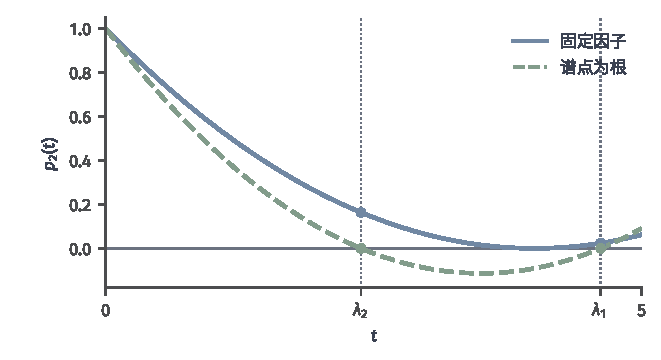
\includegraphics{figures/02-vectors-matrices-and-multivariate-calculus/03-linear-equations-and-optimization/matplotlib/learning-mechanisms/krylov-polynomial-roots.pdf}
  \caption{贯穿例$\bm A=\left[\begin{smallmatrix}4&1\\1&3\end{smallmatrix}\right]$的残差多项式。蓝线为Richardson两步的$(1-t/4)^2$，绿虚线为$1-7t/11+t^2/11$；圆点标记两个特征值处的值。二者均满足$p_2(0)=1$，只有后者在两个谱点同时为零。这是解释多项式自由度的解析对照，实际算法不需要预先知道特征值。}
  \label{fig:solver-krylov-polynomial-roots}
\end{figure}

\paragraph{选择策略}
实际计算中不知道特征值，不能像上例那样直接写出根。各方法改用可以计算的准则，在$\mathcal P_k$中隐式地选出$p_k$。准则所衡量的对象有两个。

一个是\emph{误差}
\begin{equation}
 \bm e_k=\bm x_k-\bm x_\star=p_k(\bm A)\bm e_0 ,
 \label{eq:ls-krylov-error-polynomial}
\end{equation}
后一个等式由$\bm e_k=-\bm A^{-1}\bm r_k$及$\bm A^{-1}$与$p_k(\bm A)$可交换得到。

另一个是\emph{残差}
\[
 \bm r_k=\bm b-\bm A\bm x_k=p_k(\bm A)\bm r_0 ,
\]
它可以直接算出。

误差才是我们真正关心的量，但它含未知的$\bm x_\star$，一般无法直接计算。所以一般使用残差来替代对误差的估计。

按所衡量的对象，Krylov子空间方法分为四类。

\emph{第一类：使误差最小。}误差一般算不出来，只有$\bm A$对称正定时是例外。这时误差的能量范数满足
\begin{equation}
 \lVert\bm e_k\rVert_{\bm A}^2=\bm e_k^\top\bm A\bm e_k=\bm r_k^\top\bm A^{-1}\bm r_k ,
 \label{eq:ls-krylov-energy-norm-identity}
\end{equation}
即误差的能量范数等于残差在$\bm A^{-1}$下的长度，两者是同一个量。

把近似写成
\[
  \bm x_k=\bm x_0+\bm V_k\bm y ,
\]
$\bm V_k$的列是$\mathcal K_k$的一组基，上式是$\bm y$的凸二次函数，令其梯度为零，得
\begin{equation}
 \bm V_k^\top\bm A(\bm x_\star-\bm x_0-\bm V_k\bm y)=\bm V_k^\top(\bm r_0-\bm A\bm V_k\bm y)=\bm0 .
 \label{eq:ls-krylov-galerkin-condition}
\end{equation}
条件中只出现残差，不出现$\bm x_\star$。它要求残差与子空间$\mathcal K_k$正交，称为Galerkin条件。

所以在$\bm x_0+\mathcal K_k$中使误差的能量范数最小，不必知道$\bm x_\star$就能做到；所选的$p_k$使$\lVert p_k(\bm A)\bm e_0\rVert_{\bm A}$在$\mathcal P_k$中最小，同时也就使残差的$\bm A^{-1}$长度最小。共轭梯度法（第~\ref{sec:ls-conjugate-gradient}节）采用这一策略。它控制的是这两种加权长度，欧氏残差$\lVert\bm r_k\rVert_2$不必每步下降。

\emph{第二类：使残差最小。}没有对称正定性提供的保证时，一般直接要求残差的欧氏长度
\[
 \lVert\bm r_k\rVert_2=\lVert p_k(\bm A)\bm r_0\rVert_2
\]
在$\mathcal P_k$中最小。这只要求$\bm A$可逆，并且因$\mathcal K_k\subseteq\mathcal K_{k+1}$，残差长度随$k$单调不增。MINRES（第~\ref{sec:ls-minres}节）对对称矩阵、GMRES（第~\ref{sec:ls-gmres}节）对一般方阵采用这一策略；前者借对称性只用短递推，后者要保存全部基向量。

长方矩阵的最小二乘问题中，LSQR（第~\ref{sec:ls-lsqr}节）在$\mathcal K_k(\bm A^\top\bm A,\bm A^\top\bm b)$中使原残差$\lVert\bm b-\bm A\bm x_k\rVert_2$最小，残差多项式的变量换成$\bm A^\top\bm A$。

\emph{第三类：使正规残差最小。}不相容的最小二乘问题中，原残差不会趋于零，判断是否已到最小二乘解要看正规方程的残差$\bm A^\top(\bm b-\bm A\bm x_k)$。LSQR使原残差单调下降，但正规残差的长度在病态问题中可能有小幅波动，不便作为停止判据。LSMR（第~\ref{sec:ls-lsmr}节）在同一个子空间中改为使正规残差的长度$\lVert\bm A^\top(\bm b-\bm A\bm x_k)\rVert_2$最小，于是它随$k$单调不增。

\emph{第四类：由正交条件确定。}对非对称矩阵，第二类准则需要保存全部基向量。若希望像对称情形那样只用短递推，常规的残差无法给出三项递推，于是BiCG（第~\ref{sec:ls-bicg}节）另取一个向量$\widetilde{\bm r}_0$，称为\term{影子残差}（shadow residual），并生成$\bm A^\top$的Krylov子空间
\begin{equation}
 \mathcal L_k=\mathcal K_k(\bm A^\top,\widetilde{\bm r}_0)=\operatorname{span}\{\widetilde{\bm r}_0,\bm A^\top\widetilde{\bm r}_0,\ldots,(\bm A^\top)^{k-1}\widetilde{\bm r}_0\}.
 \label{eq:ls-krylov-test-space}
\end{equation}
它不再寻找使某个长度最小的$p_k$，而是规定残差必须与$\mathcal L_k$正交，这样的$\mathcal L_k$称为\term{检验空间}（test space）。设$\bm W_k$的列是$\mathcal L_k$的一组基，条件$\bm W_k^\top(\bm r_0-\bm A\bm V_k\bm y)=\bm0$就是$k$阶方程
\begin{equation}
 (\bm W_k^\top\bm A\bm V_k)\,\bm y=\bm W_k^\top\bm r_0 ,
 \label{eq:ls-krylov-projection}
\end{equation}
解出$\bm y$，就由代数关系唯一地确定了$p_k$。

检验空间与子空间不同的这类条件，统称为Petrov--Galerkin条件；第一类中的Galerkin条件是$\mathcal L_k=\mathcal K_k$的特例。这样选出的$p_k$不使任何长度最小，残差可能剧烈起伏，方程~\eqref{eq:ls-krylov-projection}的系数矩阵也可能奇异而使迭代中断。

BiCGSTAB（第~\ref{sec:ls-bicgstab}节）在BiCG的多项式上每步再乘一个一次因子$1-\omega_jt$，并按局部的残差极小化选取$\omega_j$，以减缓这种起伏。这里不展开这一条件的几何意义，只把它作为选择$p_k$的第四种方式。

综上，本章的方法按选择$p_k$的准则分为四类：使误差（能量范数）最小的CG，使残差最小的MINRES、GMRES与LSQR，使正规残差最小的LSMR，以及由与影子子空间正交确定$p_k$的BiCG与BiCGSTAB。

\section{Arnoldi正交化}
\label{sec:ls-arnoldi}

第~\ref{sec:ls-krylov-subspaces}节的选解准则都要在$\mathcal K_k(\bm A,\bm r_0)$中计算，而幂向量$\bm r_0,\bm A\bm r_0,\ldots$随次数增加趋于同一方向，不宜直接作基。对一般方阵，\term{Arnoldi正交化}（Arnoldi process）逐个生成这个子空间的一组标准正交基，并把$\bm A$在子空间上的作用记录为一个上Hessenberg小矩阵。

下面先说明它的任务与正交化方法，再写出计算过程，然后分析所得结果的含义，最后说明它怎样用于求解方程。后两节的Lanczos过程与Golub--Kahan双对角化分别是它在对称矩阵与长方矩阵上的变形。

\subsection{主要思想}

给定方阵$\bm A\in\mathbb R^{d\times d}$，不要求对称，只假定$\bm A$乘向量容易计算；再给定初始残差$\bm r_0\ne\bm 0$与迭代步数$k$。Arnoldi正交化要生成一组标准正交向量$\bm v_1,\ldots,\bm v_k$，使对每个$j\le k$，前$j$个向量张成$\mathcal K_j(\bm A,\bm r_0)$。

\paragraph{修正Gram--Schmidt正交化}

第一个向量取初始残差的方向，
\begin{equation}
 \bm v_1=\frac{\bm r_0}{\lVert\bm r_0\rVert_2},
 \label{eq:ls-arnoldi-start}
\end{equation}

设已有标准正交的$\bm v_1,\ldots,\bm v_j$，它们张成$\mathcal K_j$。$\bm v_j$在$\bm A^{j-1}\bm r_0$上的系数非零，所以
\[
  \mathcal K_{j+1}=\mathcal K_j+\operatorname{span}\{\bm A\bm v_j\} ,
\]
$\mathcal K_{j+1}$比$\mathcal K_j$多出的方向来自$\bm A\bm v_j$。

于是先作$\bm w=\bm A\bm v_j$，再用第~\ref{sec:ls-qr-method}节的修正Gram--Schmidt把它在已有基向量上的分量逐个扣除，对$i=1,\ldots,j$依次计算
\begin{equation}
 h_{i,j}=\bm v_i^\top\bm w,\qquad \bm w\leftarrow\bm w-h_{i,j}\bm v_i .
 \label{eq:ls-arnoldi-coefficients}
\end{equation}
每个$h_{i,j}$都用已经扣除前面分量的当前$\bm w$求内积。

此前扣除的$\bm v_1,\ldots,\bm v_{i-1}$与$\bm v_i$正交，所以精确算术下这与$h_{i,j}=\bm v_i^\top\bm A\bm v_j$相同，有限精度下逐个扣除保持正交性更好。

扣除完毕后，余项$\bm w$与$\bm v_1,\ldots,\bm v_j$都正交，再把它归一化，
\begin{equation}
 h_{j+1,j}=\lVert\bm w\rVert_2,\qquad \bm v_{j+1}=\frac{\bm w}{h_{j+1,j}}\quad(h_{j+1,j}\ne0),
 \label{eq:ls-arnoldi-normalize}
\end{equation}
就得到下一个基向量。

把扣除的分量加回去，每个$\bm A\bm v_j$都是前$j+1$个基向量的组合：
\begin{equation}
 \bm A\bm v_j=\sum_{i=1}^{j+1}h_{i,j}\bm v_i .
 \label{eq:ls-arnoldi-column}
\end{equation}

\paragraph{与全部旧基向量耦合}
一般方阵的系数$h_{i,j}=\bm v_i^\top\bm A\bm v_j$（$i\le j$）通常都不为零，新向量与此前的全部基向量耦合：第$j$轮要与$\bm v_1,\ldots,\bm v_j$逐个求内积并扣除，整组基都须保存。第~\ref{sec:ls-lanczos}节将说明，$\bm A$对称时其中只有最近的两项非零，扣除可以缩短为三项递推。

\subsection{计算过程}

按上一小节的推导，Arnoldi正交化每轮作一次矩阵乘向量，把结果对已有基向量逐个扣除，再把余项归一化。下面写出计算中用到的变量、它们怎样初始化、每轮怎样更新。下面用例~\ref{ex:ls-stationary-running-example}的以下数据逐步演示：
\[
 \bm A=\begin{bmatrix}4&1\\1&3\end{bmatrix},\qquad \bm b=\begin{bmatrix}1\\2\end{bmatrix}.
\]
取$\bm x_0=\bm 0$，于是$\bm r_0=\bm b$，步数取$k=2$。

\paragraph{变量}
\begin{itemize}
 \item $\bm v_1,\ldots,\bm v_j\in\mathbb R^d$：已生成的标准正交基向量，全部保存。
 \item $\bm w\in\mathbb R^d$：工作向量，先存$\bm A\bm v_j$，再在原处逐个扣除已有分量，成为余项。
 \item $h_{1,j},\ldots,h_{j+1,j}$：第$j$轮的系数，即上Hessenberg矩阵$\overline{\bm H}_k$的第$j$列。
 \item $j$：轮次。
\end{itemize}

\paragraph{初始化}
把第一个基向量初始化为初始残差的方向，轮次初始化为$1$：
\[
 \bm v_1=\frac{\bm r_0}{\lVert\bm r_0\rVert_2},\qquad j=1 .
\]
例中$\lVert\bm r_0\rVert_2=\sqrt5$，
\[
 \bm v_1=\frac1{\sqrt5}\begin{bmatrix}1\\2\end{bmatrix}.
\]

\paragraph{每轮更新}
在第$j$轮：
\begin{enumerate}
 \item \textbf{乘矩阵。}计算
 \[
  \bm w=\bm A\bm v_j .
 \]
 例中第一轮
 \[
  \bm w=\bm A\bm v_1=(6,7)^\top/\sqrt5 .
 \]

 \item \textbf{逐个扣除已有分量。}按式~\eqref{eq:ls-arnoldi-coefficients}，对$i=1,\ldots,j$依次计算
 \[
  h_{i,j}=\bm v_i^\top\bm w,\qquad \bm w\leftarrow\bm w-h_{i,j}\bm v_i ,
 \]
 每个内积都用已扣除前面分量的当前$\bm w$。例中第一轮只有$i=1$：
 \[
  h_{1,1}=\frac{1\cdot6+2\cdot7}{5}=4,\qquad
  \bm w=\frac1{\sqrt5}\Bigl(\begin{bmatrix}6\\7\end{bmatrix}-4\begin{bmatrix}1\\2\end{bmatrix}\Bigr)=\frac1{\sqrt5}\begin{bmatrix}2\\-1\end{bmatrix}.
 \]

 \item \textbf{归一化。}按式~\eqref{eq:ls-arnoldi-normalize}计算
 \[
  h_{j+1,j}=\lVert\bm w\rVert_2,\qquad \bm v_{j+1}=\frac{\bm w}{h_{j+1,j}} .
 \]
 例中第一轮
 \[
  h_{2,1}=1,\qquad \bm v_2=\frac1{\sqrt5}\begin{bmatrix}2\\-1\end{bmatrix}.
 \]
 然后令$j\leftarrow j+1$，进入下一轮。
 
 例中第二轮先乘矩阵，得
 \[
  \bm w=\bm A\bm v_2=(7,-1)^\top/\sqrt5 ,
 \]
 再依次扣除两个方向：
 \[
  \begin{aligned}
  h_{1,2}&=\frac{7-2}{5}=1,&\qquad \bm w&=\frac1{\sqrt5}\begin{bmatrix}6\\-3\end{bmatrix};\\
  h_{2,2}&=\frac{12+3}{5}=3,&\qquad \bm w&=\bm 0 ,
  \end{aligned}
 \]
 于是$h_{3,2}=0$。

 \item \textbf{停止。}当$h_{j+1,j}=0$（实际中低于按输入尺度取定的阈值）时，$\bm A\bm v_j$已落在现有空间中，Krylov子空间不再扩张，不作归一化，退出迭代；否则做满$k$轮后退出。例中第二轮$h_{3,2}=0$，二维空间已经用尽，退出迭代。
\end{enumerate}
若扣除后的$\lVert\bm w\rVert_2$远小于扣除前的$\lVert\bm A\bm v_j\rVert_2$，说明发生了大量相消，余项可能已带有旧方向的成分。这时在归一化之前对已有基再投影一遍，得修正量$\delta_i=\bm v_i^\top\bm w$，令$\bm w\leftarrow\bm w-\delta_i\bm v_i$，并把它加回$h_{i,j}\leftarrow h_{i,j}+\delta_i$。

例中第一轮扣除前长度为$\sqrt{17}\approx4.12$，扣除后为$1$，相消不严重，不需再正交化。

最终得到标准正交基$\bm v_1,\bm v_2$与各轮系数组成的小矩阵。例中
\[
 \bm V_2=\frac1{\sqrt5}\begin{bmatrix}1&2\\2&-1\end{bmatrix},\qquad
 \bm H_2=\begin{bmatrix}h_{1,1}&h_{1,2}\\h_{2,1}&h_{2,2}\end{bmatrix}=\begin{bmatrix}4&1\\1&3\end{bmatrix},
\]
它们满足
\[
 \bm A\bm V_2=\bm V_2\bm H_2 .
\]

\subsection{算法分析}

\paragraph{基矩阵与投影矩阵}
把各步得到的标准正交基并排，记
\begin{equation}
 \bm V_k=[\bm v_1,\ldots,\bm v_k]\in\mathbb R^{d\times k}.
 \label{eq:ls-arnoldi-basis-matrix}
\end{equation}
它的行数是原矩阵的维数$d$，列数是迭代步数$k$。通常$k\ll d$，$\bm V_k$是一个瘦长矩阵：它的列张成$\mathcal K_k$，把$d$维空间中的这个$k$维子空间用$k$个坐标表示出来。

把$j=1,\ldots,k$的列关系~\eqref{eq:ls-arnoldi-column}按列并排写出，得到矩阵形式
\begin{equation}
 \bm A\bm V_k=\bm V_{k+1}\overline{\bm H}_k=\bm V_k\bm H_k+h_{k+1,k}\bm v_{k+1}\bm e_k^\top ,
 \label{eq:ls-arnoldi-relation}
\end{equation}
其中$\overline{\bm H}_k\in\mathbb R^{(k+1)\times k}$在$i\le j+1$处的元素为$h_{i,j}$、其余为零，$\bm H_k$是它去掉末行所得的$k$阶方阵。以$k=3$为例，
\[
 \bm A\begin{bmatrix}\bm v_1&\bm v_2&\bm v_3\end{bmatrix}
 =\begin{bmatrix}\bm v_1&\bm v_2&\bm v_3&\bm v_4\end{bmatrix}
 \begin{bmatrix}h_{1,1}&h_{1,2}&h_{1,3}\\h_{2,1}&h_{2,2}&h_{2,3}\\0&h_{3,2}&h_{3,3}\\0&0&h_{4,3}\end{bmatrix}.
\]
$\bm A\bm v_j$只用到前$j+1$个基向量，所以第$j$列在第$j+1$行以下全为零；这种\emph{上Hessenberg}形是生成过程的结果。图~\ref{fig:ls-arnoldi-relation-shapes}画出了式~\eqref{eq:ls-arnoldi-relation}中各矩阵的形状。

\begin{figure}[htbp]
  \centering
  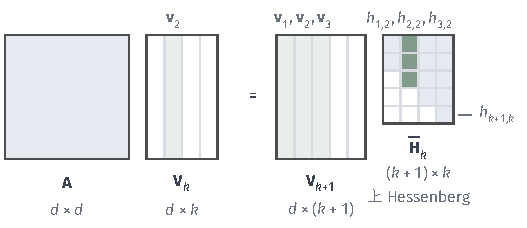
\includegraphics[width=89.098mm]{figures/01-basic-mathematics/03-vectors-matrices-and-multivariate-functions/tikz/c5-arnoldi-relation-shapes/figure.pdf}
  \caption{Arnoldi关系$\bm A\bm V_k=\bm V_{k+1}\overline{\bm H}_k$中各矩阵的形状（示意$d=7$、$k=4$）。$\overline{\bm H}_k$的非零元（浅蓝）只出现在主对角线、其上方和紧邻的下次对角线上，是上Hessenberg矩阵，末行只剩$h_{k+1,k}$。绿色标出第$j=2$列：$\bm A\bm v_2$只用到$\bm v_1,\bm v_2,\bm v_3$，系数是$\overline{\bm H}_k$第2列的前三个元素。}
  \label{fig:ls-arnoldi-relation-shapes}
\end{figure}

左乘$\bm V_k^\top$，并用$\bm V_k^\top\bm V_k=\bm I$与$\bm V_k^\top\bm v_{k+1}=\bm 0$，得
\begin{equation}
 \bm H_k=\bm V_k^\top\bm A\bm V_k .
 \label{eq:ls-arnoldi-projection}
\end{equation}
所以$\bm H_k$是$\bm A$在$\mathcal K_k$上的投影：若$\bm z=\bm V_k\bm y$是子空间中的向量，则$\bm A\bm z$在子空间中的分量的坐标为$\bm H_k\bm y$，伸出子空间的部分只沿$\bm v_{k+1}$一个方向，大小由$h_{k+1,k}$记录。

图中$\bm V_{k+1}$只比$\bm V_k$多一列，而$\overline{\bm H}_k$只有$k+1$行：$d$维矩阵在子空间上的作用，就这样被压缩成一个$k$阶的上Hessenberg矩阵。

\paragraph{正确性}
上面的论证用到了“此前各步的基已经标准正交”。下面的定理用归纳法确认这一点，并给出终止的情形。

\begin{theorem}[Arnoldi关系]
\label{thm:ls-arnoldi-relation}
在精确算术下按式~\eqref{eq:ls-arnoldi-coefficients}与\eqref{eq:ls-arnoldi-normalize}执行$k$轮Arnoldi正交化，且前$k-1$轮的$h_{j+1,j}$均非零。若$h_{k+1,k}\ne0$，则$\bm v_1,\ldots,\bm v_{k+1}$标准正交，$\bm v_1,\ldots,\bm v_j$张成$\mathcal K_j$（$j\le k+1$），关系~\eqref{eq:ls-arnoldi-relation}成立，并且$\bm H_k=\bm V_k^\top\bm A\bm V_k$。若$h_{k+1,k}=0$，则$\bm v_1,\ldots,\bm v_k$标准正交，$\bm A\bm V_k=\bm V_k\bm H_k$，$\mathcal K_k$在$\bm A$下不变；$\bm A$非奇异时精确解$\bm x_\star$属于$\bm x_0+\mathcal K_k$。
\end{theorem}

\begin{proof}
依次证明正交性、张成关系与矩阵关系，最后处理子空间不再扩张的情形。

\emph{正交性。}对$j$归纳，设$\bm v_1,\ldots,\bm v_j$标准正交。第$i$次扣除后$\bm w\perp\bm v_i$，此后扣除的方向$\bm v_{i+1},\ldots,\bm v_j$都与$\bm v_i$正交，不破坏这一关系，所以最终余项与$\bm v_1,\ldots,\bm v_j$都正交。$h_{j+1,j}\ne0$时归一化得到单位向量$\bm v_{j+1}$，与前$j$个正交。

\emph{张成与矩阵关系。}$\bm v_1\in\mathcal K_1$；若$\bm v_1,\ldots,\bm v_j\in\mathcal K_j$，则
\[
 \bm v_{j+1}\in\operatorname{span}\{\bm A\bm v_j,\bm v_1,\ldots,\bm v_j\}\subseteq\mathcal K_{j+1},
\]
$j+1$个标准正交向量落在维数不超过$j+1$的$\mathcal K_{j+1}$中，因而张成它。由式~\eqref{eq:ls-arnoldi-normalize}，扣除完毕后的余项就是$h_{j+1,j}\bm v_{j+1}$，把扣除的分量加回即得列关系~\eqref{eq:ls-arnoldi-column}，并排写出即是式~\eqref{eq:ls-arnoldi-relation}。左乘$\bm V_k^\top$，并用$\bm V_k^\top\bm V_k=\bm I$与$\bm V_k^\top\bm v_{k+1}=\bm 0$，得$\bm H_k=\bm V_k^\top\bm A\bm V_k$。

\emph{不再扩张的情形。}若$h_{k+1,k}=0$，第$k$列成为$\bm A\bm v_k=\sum_{i\le k}h_{i,k}\bm v_i$，于是$\bm A\bm V_k=\bm V_k\bm H_k$，$\bm A\mathcal K_k\subseteq\mathcal K_k$。$\bm A$非奇异时它在有限维空间$\mathcal K_k$上是单射，因而也是满射；$\bm r_0\in\mathcal K_k$，故有$\bm z\in\mathcal K_k$使$\bm A\bm z=\bm r_0$，$\bm x_\star=\bm x_0+\bm z$。
\end{proof}

$\mathcal K_k$的维数不超过$d$，所以至多$d$轮出现$h_{k+1,k}=0$。这时精确解已在候选集合中，使用这组基的求解器在这一步得到精确解，但仍须用原残差确认。

\paragraph{数值敏感度}
有限精度下基的正交性会逐渐损失，判断与补救办法沿用第~\ref{sec:ls-qr-method}节对修正Gram--Schmidt的讨论，必要时按“每轮的更新”所述再正交化。再正交化要用到全部已保存的基向量，Arnoldi正交化本来就保存它们，所以这一补救的代价只是多做一遍投影。

\paragraph{计算代价}
每轮一次$\bm A$乘向量。第$j$轮的扣除要作$j$次内积与$j$次向量更新，约$4dj$次浮点运算，$k$轮合计约$2dk^2$次；保存$\bm V_{k+1}$约需$(k+1)d$个数。两者都随轮数增长，原因是整组基都要保存并参与扣除。本过程只负责生成候选空间，收敛快慢由调用它的求解器在子空间中采用的选解准则决定。

\subsection{应用}
\label{sec:ls-arnoldi-application}

有了基与投影矩阵，就可以在子空间中求解方程。把近似写成
\[
 \bm x_k=\bm x_0+\bm V_k\bm y ,
\]
$\bm y\in\mathbb R^k$是子空间中的坐标。由$\bm r_0=\lVert\bm r_0\rVert_2\bm v_1=\bm V_{k+1}\lVert\bm r_0\rVert_2\bm e_1$与关系~\eqref{eq:ls-arnoldi-relation}，残差可以写成
\begin{equation}
 \bm r_0-\bm A\bm V_k\bm y=\bm V_{k+1}\bigl(\lVert\bm r_0\rVert_2\bm e_1-\overline{\bm H}_k\bm y\bigr),
 \label{eq:ls-arnoldi-residual-coordinates}
\end{equation}
其中$\bm e_1\in\mathbb R^{k+1}$。$d$维的残差由此用$k+1$个坐标表示出来。第~\ref{sec:ls-krylov-selection-criteria}节的准则都可以在这个小问题上实现。

按Galerkin条件，要求残差与$\mathcal K_k$正交，即$\bm V_k^\top(\bm r_0-\bm A\bm V_k\bm y)=\bm 0$。由$\bm H_k=\bm V_k^\top\bm A\bm V_k$，这就是$k$阶上Hessenberg方程组
\begin{equation}
 \bm H_k\bm y=\lVert\bm r_0\rVert_2\,\bm e_1 ,
 \label{eq:ls-arnoldi-galerkin-system}
\end{equation}
这里$\bm e_1\in\mathbb R^k$。

不过对非对称矩阵，Galerkin条件没有极小性，$\bm H_k$也可能奇异。按极小残差条件，则因$\bm V_{k+1}$的列标准正交、不改变长度，在子空间中求残差最小的坐标化为$(k+1)\times k$的小型最小二乘问题
\begin{equation}
 \min_{\bm y}\bigl\lVert\lVert\bm r_0\rVert_2\bm e_1-\overline{\bm H}_k\bm y\bigr\rVert_2 ,
 \label{eq:ls-arnoldi-minimal-residual-problem}
\end{equation}
它对任何非奇异的$\bm A$都有唯一解。这就是GMRES（第~\ref{sec:ls-gmres}节）的做法；$\overline{\bm H}_k$是上Hessenberg矩阵，每增加一列只需一次新的Givens旋转就能延续三角化。

这两种用法都要用$\bm V_k$还原$\bm x_k$，整组基须一直保存，存储与正交化工作随步数增长。实际计算因此常在做满$m$步后停下，以当前近似为新起点重新开始生成基，即\emph{重启}；它限制了存储，代价是失去跨周期的最优性。

\section{Lanczos正交化}
\label{sec:ls-lanczos}

第~\ref{sec:ls-arnoldi}节的Arnoldi正交化对一般方阵生成$\mathcal K_k(\bm A,\bm r_0)$的标准正交基，代价是每轮都要与全部旧基向量正交化。$\bm A$对称时，其中大部分系数自动为零。\term{Lanczos过程}（Lanczos process）就是Arnoldi正交化在对称矩阵上的简化：每轮只扣除两个方向，就生成同一组标准正交基，并把$\bm A$在子空间上的作用记录为一个对称三对角小矩阵。下面先推出三项递推，再写出计算过程，然后分析所得结果，最后说明它怎样用于求解方程；与Arnoldi正交化相同的论证只作引用。

\subsection{主要思想}

Lanczos过程的任务与Arnoldi正交化相同，只是矩阵对称：给定对称矩阵$\bm A\in\mathbb R^{d\times d}$、初始残差$\bm r_0\ne\bm 0$与步数$k$，生成标准正交向量$\bm v_1,\ldots,\bm v_k$，使前$j$个向量张成$\mathcal K_j(\bm A,\bm r_0)$，第一个向量取$\bm v_1=\bm r_0/\lVert\bm r_0\rVert_2$。

\paragraph{三项递推}
从第~\ref{sec:ls-arnoldi}节的系数出发。精确算术下，Arnoldi正交化在第$j$轮扣除的系数为
\[
 h_{i,j}=\bm v_i^\top\bm A\bm v_j\quad(i\le j),
\]
并且由列关系~\eqref{eq:ls-arnoldi-column}，每个$\bm A\bm v_i$都是$\bm v_1,\ldots,\bm v_{i+1}$的组合。$\bm A$对称时，
\[
 h_{i,j}=\bm v_i^\top\bm A\bm v_j=(\bm A\bm v_i)^\top\bm v_j .
\]
当$i+1<j$时，$\bm A\bm v_i$所含的$\bm v_1,\ldots,\bm v_{i+1}$都与$\bm v_j$正交，所以$h_{i,j}=0$；

当$i=j-1$时，$h_{j-1,j}=(\bm A\bm v_{j-1})^\top\bm v_j$恰是上一轮的归一化系数$h_{j,j-1}$。

于是第$j$轮只剩对角系数$h_{j,j}$与归一化系数$h_{j+1,j}$需要计算。记
\begin{equation}
 a_j=h_{j,j},\qquad \gamma_j=h_{j+1,j},
 \label{eq:ls-lanczos-coefficients}
\end{equation}
并约定$\bm v_0=\bm 0$、$\gamma_0=0$，列关系~\eqref{eq:ls-arnoldi-column}化为
\begin{equation}
 \bm A\bm v_j=\gamma_{j-1}\bm v_{j-1}+a_j\bm v_j+\gamma_j\bm v_{j+1},\qquad a_j=\bm v_j^\top\bm A\bm v_j ,
 \label{eq:ls-arnoldi-lanczos}
\end{equation}
这就是\term{Lanczos三项递推}（Lanczos recurrence）。计算新向量时只需用到紧邻的三个量$\bm A\bm v_j$、$\bm v_j$与$\bm v_{j-1}$，不必保存整组基。

图~\ref{fig:solver-lanczos-three-directions}把三项递推与三对角形状对应起来。固定第$j$列时，只需紧邻的三个基方向；其他位置的系数因对称性和正交性为零。

\begin{figure}[!htb]
  \centering
  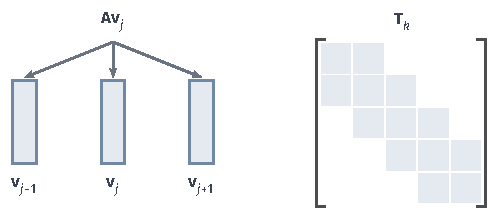
\includegraphics{figures/02-vectors-matrices-and-multivariate-calculus/03-linear-equations-and-optimization/tikz/learning-mechanisms/lanczos-three-directions.pdf}
  \caption{Lanczos过程在精确算术下的局部关系。左侧$\bm A\bm v_j$由$\bm v_{j-1},\bm v_j,\bm v_{j+1}$三个方向组成；右侧对称三对角矩阵$\bm T_k$只在主对角线和相邻两条对角线上可能非零。有限精度下可能需要重新正交化，图示不代表舍入后仍自动保持全局正交。}
  \label{fig:solver-lanczos-three-directions}
\end{figure}

\subsection{算法实现}

由三项递推~\eqref{eq:ls-arnoldi-lanczos}移项，每轮作一次矩阵乘向量，扣除两个方向，再把余项归一化。下面写出计算中用到的变量、它们怎样初始化、每轮怎样更新。下面用例~\ref{ex:ls-stationary-running-example}的以下数据逐步演示：
\[
 \bm A=\begin{bmatrix}4&1\\1&3\end{bmatrix},\qquad \bm b=\begin{bmatrix}1\\2\end{bmatrix}.
\]
取$\bm x_0=\bm 0$，于是$\bm r_0=\bm b$，步数取$k=2$。

\paragraph{变量}
\begin{itemize}
 \item $\bm v_{j-1},\bm v_j\in\mathbb R^d$：上一个与当前基向量，只保存这两个。
 \item $\bm w\in\mathbb R^d$：工作向量，先存$\bm A\bm v_j$，再在原处扣除两个方向，成为余项。
 \item $a_j$：第$j$个对角元。
 \item $\gamma_j$：第$j$个次对角元，也是$\bm v_{j+1}$的归一化系数；$\gamma_{j-1}$留到本轮扣除时使用。
 \item $j$：轮次。
\end{itemize}

\paragraph{初始化}
把上一个基向量初始化为零向量，$\gamma_0$初始化为零，第一个基向量初始化为初始残差的方向，轮次初始化为$1$：
\[
 \bm v_0=\bm 0,\qquad \gamma_0=0,\qquad \bm v_1=\frac{\bm r_0}{\lVert\bm r_0\rVert_2},\qquad j=1 .
\]
例中$\lVert\bm r_0\rVert_2=\sqrt5$，
\[
 \bm v_1=\frac1{\sqrt5}\begin{bmatrix}1\\2\end{bmatrix}.
\]

\paragraph{每轮更新}
在第$j$轮：
\begin{enumerate}
 \item \textbf{乘矩阵。}计算
 \[
  \bm w=\bm A\bm v_j .
 \]
 例中第一轮
 \[
   \bm w=\bm A\bm v_1=(6,7)^\top/\sqrt5 .
 \]

 \item \textbf{求对角元。}计算
 \[
  a_j=\bm v_j^\top\bm w .
 \]
 例中第一轮
 \[
   a_1=(1\cdot6+2\cdot7)/5=4 .
 \]

 \item \textbf{扣除两个方向。}计算
 \[
  \bm w\leftarrow\bm w-a_j\bm v_j-\gamma_{j-1}\bm v_{j-1} .
 \]
 例中第一轮$\gamma_0=0$，
 \[
  \bm w=\frac1{\sqrt5}\Bigl(\begin{bmatrix}6\\7\end{bmatrix}-4\begin{bmatrix}1\\2\end{bmatrix}\Bigr)=\frac1{\sqrt5}\begin{bmatrix}2\\-1\end{bmatrix}.
 \]

 \item \textbf{归一化。}计算
 \[
  \gamma_j=\lVert\bm w\rVert_2,\qquad \bm v_{j+1}=\frac{\bm w}{\gamma_j} .
 \]
 
 例中第一轮
 \[
  \gamma_1=1,\qquad \bm v_2=\frac1{\sqrt5}\begin{bmatrix}2\\-1\end{bmatrix}.
 \]
 然后令$j\leftarrow j+1$：$\bm v_j$成为下一轮的“上一个基向量”，$\bm v_{j+1}$成为“当前基向量”。

 例中第二轮先乘矩阵，得
 \[
  \bm w=\bm A\bm v_2=(7,-1)^\top/\sqrt5 ,
 \]
 再求对角元，
 \[
  a_2=\frac{14+1}{5}=3 .
 \]
 扣除$3\bm v_2$与$\gamma_1\bm v_1$后
 \[
  \bm w=\frac1{\sqrt5}\Bigl(\begin{bmatrix}7\\-1\end{bmatrix}-3\begin{bmatrix}2\\-1\end{bmatrix}-\begin{bmatrix}1\\2\end{bmatrix}\Bigr)=\bm 0 ,
 \]
 于是$\gamma_2=0$。

 \item \textbf{停止。}当$\gamma_j=0$（实际中低于按输入尺度取定的阈值）时，$\bm A\bm v_j$已落在现有空间中，Krylov子空间不再扩张，不作归一化，退出迭代；否则做满$k$轮后退出。例中第二轮$\gamma_2=0$，二维空间已经用尽，退出迭代。
\end{enumerate}
第1—4步合起来就是
\begin{equation}
 \begin{aligned}
 \bm w&=\bm A\bm v_j, & a_j&=\bm v_j^\top\bm w,\\
 \hat{\bm w}&=\bm w-a_j\bm v_j-\gamma_{j-1}\bm v_{j-1},\\
 \gamma_j&=\lVert\hat{\bm w}\rVert_2, & \bm v_{j+1}&=\hat{\bm w}/\gamma_j .
 \end{aligned}
 \label{eq:ls-lanczos-step}
\end{equation}
实际计算中也常先扣除$\gamma_{j-1}\bm v_{j-1}$，再用扣除后的向量求$a_j$：精确算术下结果相同，这与修正Gram--Schmidt的做法一致，有限精度下正交性略好。

最终得到标准正交基$\bm v_1,\bm v_2$与各轮系数组成的三对角矩阵。例中
\[
 \bm V_2=\frac1{\sqrt5}\begin{bmatrix}1&2\\2&-1\end{bmatrix},\qquad
 \bm T_2=\begin{bmatrix}a_1&\gamma_1\\\gamma_1&a_2\end{bmatrix}=\begin{bmatrix}4&1\\1&3\end{bmatrix},
\]
它们满足
\[
 \bm A\bm V_2=\bm V_2\bm T_2 .
\]
逐列核对：
\[
 \begin{gathered}
 4(1,2)^\top+(2,-1)^\top=(6,7)^\top,\\
 (1,2)^\top+3(2,-1)^\top=(7,-1)^\top ,
 \end{gathered}
\]
两边同除以$\sqrt5$即是$\bm A\bm v_1$与$\bm A\bm v_2$。

结果与第~\ref{sec:ls-arnoldi}节对同一矩阵算出的$\bm H_2$相同，但这里每轮只扣除了两个方向。

\subsection{算法分析}

\paragraph{基矩阵与投影矩阵}
与第~\ref{sec:ls-arnoldi}节一样，把各步的基并排成瘦长矩阵$\bm V_k=[\bm v_1,\ldots,\bm v_k]\in\mathbb R^{d\times k}$，它的列张成$\mathcal K_k$。把$j=1,\ldots,k$的递推式~\eqref{eq:ls-arnoldi-lanczos}按列并排写出，得到矩阵形式
\begin{equation}
 \bm A\bm V_k=\bm V_k\bm T_k+\gamma_k\bm v_{k+1}\bm e_k^\top=\bm V_{k+1}\overline{\bm T}_k ,
 \label{eq:ls-arnoldi-tridiagonal}
\end{equation}
其中
\begin{equation}
 \bm T_k=\begin{bmatrix}
 a_1&\gamma_1&&\\
 \gamma_1&a_2&\ddots&\\
 &\ddots&\ddots&\gamma_{k-1}\\
 &&\gamma_{k-1}&a_k
 \end{bmatrix},
 \label{eq:ls-lanczos-tridiagonal-matrix}
\end{equation}
$\overline{\bm T}_k$是在$\bm T_k$下方添一行$\gamma_k\bm e_k^\top$所得的$(k+1)\times k$矩阵。

左乘$\bm V_k^\top$，并用$\bm V_k^\top\bm V_k=\bm I$与$\bm V_k^\top\bm v_{k+1}=\bm 0$，得
\begin{equation}
 \bm T_k=\bm V_k^\top\bm A\bm V_k .
 \label{eq:ls-lanczos-projection}
\end{equation}
这正是Arnoldi关系~\eqref{eq:ls-arnoldi-relation}在对称情形下的形式：
\[
  \overline{\bm H}_k=\overline{\bm T}_k,\qquad \bm H_k=\bm T_k .
\]

$\bm T_k$同样是$\bm A$在$\mathcal K_k$上的投影，即子空间中向量的像在子空间中的坐标由$\bm T_k$给出；不同的是，它不仅是上Hessenberg矩阵，而且对称，因而是三对角的。

$d$维对称矩阵在子空间上的作用，就这样被压缩成一个$k$阶对称三对角矩阵，只需$2k-1$个数$a_1,\ldots,a_k$与$\gamma_1,\ldots,\gamma_{k-1}$记录。

\paragraph{正确性}
推导三项递推时用到了“此前各步的基已经标准正交”，这是由完整扣除保证的；只扣除两项时需要重新确认。下面的定理用归纳法证明这一点，并给出终止的情形。

\begin{theorem}[Lanczos关系]
\label{thm:ls-arnoldi-lanczos}
设$\bm A$对称，$\bm r_0\ne\bm 0$，在精确算术下按式~\eqref{eq:ls-lanczos-step}执行$k$轮，且$\gamma_1,\ldots,\gamma_{k-1}$均非零。若$\gamma_k\ne0$，则$\bm v_1,\ldots,\bm v_{k+1}$标准正交，$\bm v_1,\ldots,\bm v_j$张成$\mathcal K_j$（$j\le k+1$），关系~\eqref{eq:ls-arnoldi-tridiagonal}成立，并且$\bm T_k=\bm V_k^\top\bm A\bm V_k$。若$\gamma_k=0$，则$\bm v_1,\ldots,\bm v_k$标准正交，$\bm A\bm V_k=\bm V_k\bm T_k$，$\mathcal K_k$在$\bm A$下不变；$\bm A$非奇异时精确解$\bm x_\star$属于$\bm x_0+\mathcal K_k$。
\end{theorem}

\begin{proof}
依次证明正交性、张成关系与矩阵关系，最后处理子空间不再扩张的情形。

\emph{正交性。}对$j$归纳，设$\bm v_1,\ldots,\bm v_j$标准正交，且对$i<j$式~\eqref{eq:ls-arnoldi-lanczos}成立。只需证明扣除后的$\hat{\bm w}=\bm A\bm v_j-a_j\bm v_j-\gamma_{j-1}\bm v_{j-1}$与$\bm v_1,\ldots,\bm v_j$都正交。对$i=j$，由$a_j=\bm v_j^\top\bm A\bm v_j$，$\bm v_j^\top\hat{\bm w}=0$。对$i<j$，由对称性$\bm v_i^\top\bm A\bm v_j=(\bm A\bm v_i)^\top\bm v_j$，而$\bm A\bm v_i=\gamma_{i-1}\bm v_{i-1}+a_i\bm v_i+\gamma_i\bm v_{i+1}$，所以
\[
 \bm v_i^\top\bm A\bm v_j=\gamma_i\,\bm v_{i+1}^\top\bm v_j=
 \begin{cases}\gamma_{j-1},&i=j-1,\\0,&i<j-1.\end{cases}
\]
再由$\bm v_i^\top\bm v_{j-1}$与$\bm v_i^\top\bm v_j$的取值，$i=j-1$时$\bm v_{j-1}^\top\hat{\bm w}=\gamma_{j-1}-\gamma_{j-1}=0$，$i<j-1$时三项都为零。$\gamma_j\ne0$时归一化得到单位向量$\bm v_{j+1}$，与前$j$个正交。

\emph{张成与矩阵关系。}$\bm v_1\in\mathcal K_1$；若$\bm v_{j-1},\bm v_j\in\mathcal K_j$，则
\[
 \bm v_{j+1}\in\operatorname{span}\{\bm A\bm v_j,\bm v_j,\bm v_{j-1}\}\subseteq\mathcal K_{j+1},
\]
$j+1$个标准正交向量落在维数不超过$j+1$的$\mathcal K_{j+1}$中，因而张成它。由式~\eqref{eq:ls-lanczos-step}，$\gamma_j\bm v_{j+1}$就是扣除后的余项，把扣除的两项加回即得列关系~\eqref{eq:ls-arnoldi-lanczos}，并排写出即是式~\eqref{eq:ls-arnoldi-tridiagonal}。左乘$\bm V_k^\top$，并用$\bm V_k^\top\bm V_k=\bm I$与$\bm V_k^\top\bm v_{k+1}=\bm 0$，得$\bm T_k=\bm V_k^\top\bm A\bm V_k$。

\emph{不再扩张的情形。}若$\gamma_k=0$，第$k$列成为$\bm A\bm v_k=\gamma_{k-1}\bm v_{k-1}+a_k\bm v_k$，于是$\bm A\bm V_k=\bm V_k\bm T_k$，$\bm A\mathcal K_k\subseteq\mathcal K_k$。$\bm A$非奇异时它在有限维空间$\mathcal K_k$上是单射，因而也是满射；$\bm r_0\in\mathcal K_k$，故有$\bm z\in\mathcal K_k$使$\bm A\bm z=\bm r_0$，$\bm x_\star=\bm x_0+\bm z$。
\end{proof}

定理表明，精确算术下只扣除两项与扣除全部已有分量结果相同：被省略的系数$\bm v_i^\top\bm A\bm v_j$（$i<j-1$）本来就是零。第~\ref{sec:ls-arnoldi}节对一般方阵扣除全部已有分量，得到上Hessenberg小矩阵；$\bm A$对称时它退化为这里的$\bm T_k$，两种过程给出相同的基与系数，贯穿例上两节的数值也完全一致。$\mathcal K_k$的维数不超过$d$，所以至多$d$轮出现$\gamma_k=0$。

\paragraph{数值敏感度}
有限精度下，正交性依赖的相消只近似成立。三项递推只对最近两个方向扣除，舍入引入的旧方向分量不会被去掉，并且会随迭代放大，基的正交性损失比第~\ref{sec:ls-arnoldi}节的完整正交化明显；典型的表现是$\bm T_k$的特征值中出现$\bm A$同一特征值的多个近似副本。保存全部基并再正交化可以补救，但这就失去了固定存储的优点；不保存基时，调用它的求解器只能靠真实残差复核控制结果。

\paragraph{计算代价}
每轮一次$\bm A$乘向量，此外只有两次内积（其一用于求$\gamma_j$）、两次向量更新和一次缩放，约$9d$次浮点运算；除矩阵外保存$\bm v_{j-1},\bm v_j,\bm w$三个向量，存储不随轮数增长。与Arnoldi正交化$k$轮约$2dk^2$次运算、$(k+1)d$个数的存储相比，这是利用对称性得到的主要收益。本过程只负责生成候选空间，收敛快慢由调用它的求解器在子空间中采用的选解准则决定。

\subsection{应用}
\label{sec:ls-lanczos-application}

用法与第~\ref{sec:ls-arnoldi-application}节相同：把近似写成$\bm x_k=\bm x_0+\bm V_k\bm y$，$\bm y\in\mathbb R^k$是子空间中的坐标，再按某个准则确定$\bm y$。

按Galerkin条件，$\bm V_k^\top(\bm r_0-\bm A\bm V_k\bm y)=\bm0$，由$\bm r_0=\lVert\bm r_0\rVert_2\bm v_1$与$\bm T_k=\bm V_k^\top\bm A\bm V_k$，得到$k$阶三对角方程组
\begin{equation}
 \bm T_k\bm y=\lVert\bm r_0\rVert_2\,\bm e_1 .
 \label{eq:ls-lanczos-projected-system}
\end{equation}
它只有$k\times k$大小，又是三对角的，用第~\ref{sec:ls-lu}节的消元约$O(k)$次运算即可解出；解出坐标$\bm y$后，再用$\bm V_k$还原，就得到原空间中的近似解$\bm x_k$。

这就是后面两种对称矩阵求解器的共同骨架。对称正定时，$\bm T_k$也对称正定，方程~\eqref{eq:ls-lanczos-projected-system}总有唯一解，所得近似就是CG的迭代值（第~\ref{sec:ls-conjugate-gradient}节）；CG还利用$\bm T_k$的分解随步数延伸的结构，把求解与还原合并为短递推，连基$\bm V_k$也不必保存。

对称不定时，$\bm T_k$可能奇异，MINRES（第~\ref{sec:ls-minres}节）改用$(k+1)\times k$的$\overline{\bm T}_k$，在子空间中求残差最小的坐标：
\begin{equation}
 \min_{\bm y}\bigl\lVert\lVert\bm r_0\rVert_2\bm e_1-\overline{\bm T}_k\bm y\bigr\rVert_2 .
 \label{eq:ls-lanczos-minimal-residual-problem}
\end{equation}

两者的子空间、基和三对角矩阵都来自同一个Lanczos过程，区别只在于用哪一种准则确定坐标$\bm y$。

\section{Golub--Kahan双对角化}
\label{sec:ls-bidiagonal-iteration}

第~\ref{sec:ls-arnoldi}节的Arnoldi正交化与第~\ref{sec:ls-lanczos}节的Lanczos过程都针对方阵：残差与未知量同在$d$维空间，可以把残差反复乘$\bm A$。长方或秩亏的最小二乘问题中，$\bm A\in\mathbb R^{m\times d}$的残差在$m$维的数据空间，未知量在$d$维空间，不能把残差反复乘$\bm A$；把数据空间的向量送回未知量空间的是$\bm A^\top$。

这时需要的是第~\ref{sec:ls-krylov-subspaces}节所说的Krylov空间$\mathcal K_k(\bm A^\top\bm A,\bm A^\top\bm b)$。$\bm A^\top\bm A$对称半正定，原则上可以对它作Lanczos过程，但形成$\bm A^\top\bm A$会损失信息。\term{Golub--Kahan双对角化}（Golub--Kahan bidiagonalization）交替作用$\bm A$与$\bm A^\top$，只用$\bm A\bm v$与$\bm A^\top\bm u$，就得到与对$\bm A^\top\bm A$作Lanczos过程相同的基，并把$\bm A$压缩成一个双对角小矩阵。下面先推出两项递推，再写出计算过程，然后分析所得结果，最后说明它怎样用于求解最小二乘问题。

\subsection{主要思想}

给定$\bm A\in\mathbb R^{m\times d}$（可以秩亏）、$\bm b\in\mathbb R^m$与步数$k$，取零初值，初始残差就是$\bm b$。双对角化要在数据空间生成标准正交基$\bm u_1,\ldots,\bm u_{k+1}$，在未知量空间生成与之配对的标准正交基$\bm v_1,\ldots,\bm v_k$，使前$j$个$\bm v$张成$\mathcal K_j(\bm A^\top\bm A,\bm A^\top\bm b)$。第一对向量取$\bm u_1=\bm b/\lVert\bm b\rVert_2$，$\bm v_1$取$\bm A^\top\bm u_1$的方向。两组向量属于不同的空间，各自在本空间内正交。

\paragraph{交替的两项递推}
仿照第~\ref{sec:ls-arnoldi}节，新向量都由“乘矩阵、扣除旧基向量的分量、归一化”得到，只是$\bm A$与$\bm A^\top$交替使用：$\bm u_{j+1}$由$\bm A\bm v_j$对$\bm u_1,\ldots,\bm u_j$正交化得到，$\bm v_{j+1}$由$\bm A^\top\bm u_{j+1}$对$\bm v_1,\ldots,\bm v_j$正交化得到。

设此前的基已分别标准正交。按构造，每个$\bm A^\top\bm u_i$都是$\bm v_1,\ldots,\bm v_i$的组合，每个$\bm A\bm v_i$都是$\bm u_1,\ldots,\bm u_{i+1}$的组合。

于是$\bm A\bm v_j$在$\bm u_i$上的系数为
\[
 \bm u_i^\top\bm A\bm v_j=(\bm A^\top\bm u_i)^\top\bm v_j ,
\]
当$i<j$时$\bm A^\top\bm u_i$所含的$\bm v_1,\ldots,\bm v_i$都与$\bm v_j$正交，系数为零，只剩$i=j$一项。

同样，$\bm A^\top\bm u_{j+1}$在$\bm v_i$上的系数为
\[
 \bm v_i^\top\bm A^\top\bm u_{j+1}=(\bm A\bm v_i)^\top\bm u_{j+1} ,
\]
当$i<j$时$\bm A\bm v_i$所含的$\bm u_1,\ldots,\bm u_{i+1}$都与$\bm u_{j+1}$正交，系数为零，只剩$i=j$一项。

所以每生成一个新向量只需扣除对面空间中相邻的一个方向。把扣除的系数与归一化系数记为$\alpha_i,\beta_i\ge0$，并约定$\bm v_0=\bm 0$，列关系为
\begin{equation}
 \bm A\bm v_i=\alpha_i\bm u_i+\beta_{i+1}\bm u_{i+1},\qquad
 \bm A^\top\bm u_i=\beta_i\bm v_{i-1}+\alpha_i\bm v_i .
 \label{eq:ls-golub-kahan-columns}
\end{equation}

由第二式，$\bm A\bm v_j$在$\bm u_j$上的系数$(\bm A^\top\bm u_j)^\top\bm v_j$正是$\alpha_j$；由第一式，$\bm A^\top\bm u_{j+1}$在$\bm v_j$上的系数$(\bm A\bm v_j)^\top\bm u_{j+1}$正是$\beta_{j+1}$。因此扣除用的系数就是上一步的归一化系数，不必另作内积。

与Arnoldi正交化的列关系~\eqref{eq:ls-arnoldi-column}相比，每个像只用到对面空间中的两个基向量，不必保存整组基；这与Lanczos过程只需三项的原因相同，算法分析中将看到，右侧基正是$\bm A^\top\bm A$的Lanczos基。

\subsection{计算过程}

由列关系~\eqref{eq:ls-golub-kahan-columns}移项，每轮先作一次$\bm A$乘向量、扣除一个方向并归一化，得到新的$\bm u$，再作一次$\bm A^\top$乘向量、扣除一个方向并归一化，得到新的$\bm v$。下面写出计算中用到的变量、它们怎样初始化、每轮怎样更新。下面用以下不相容的长方系统逐步演示：
\[
 \bm A=\begin{bmatrix}1&0\\0&2\\0&0\end{bmatrix},\qquad
 \bm b=\begin{bmatrix}1\\1\\1\end{bmatrix}.
\]
第三行恒为零，$\bm b$的第三个分量无法拟合；最小二乘解是$\hat{\bm x}=(1,1/2)^\top$，最优残差为$(0,0,1)^\top$。这个例子的系数都有封闭形式，第~\ref{sec:ls-lsqr}节的LSQR与第~\ref{sec:ls-lsmr}节的LSMR继续用它，以便对照。

\paragraph{变量}
\begin{itemize}
 \item $\bm u_j\in\mathbb R^m$、$\bm v_j\in\mathbb R^d$：当前的两个基向量，只保存这两个；是否保存整组基由调用者决定。
 \item $\bm p\in\mathbb R^m$、$\bm q\in\mathbb R^d$：工作向量，分别存放数据空间与未知量空间中扣除后的余项。
 \item $\alpha_j$：$\bm B_k$的第$j$个对角元，也是$\bm v_j$的归一化系数。
 \item $\beta_j$：$\bm B_k$的第$j-1$列的次对角元（$\beta_1$为$\lVert\bm b\rVert_2$），也是$\bm u_j$的归一化系数。
 \item $j$：轮次。
\end{itemize}

\paragraph{初始化}
把$\bm u_1$初始化为$\bm b$的方向，再由列关系~\eqref{eq:ls-golub-kahan-columns}第二式在$i=1$时的$\bm A^\top\bm u_1=\alpha_1\bm v_1$把$\bm v_1$初始化为$\bm A^\top\bm u_1$的方向，轮次初始化为$1$：
\begin{equation}
 \begin{gathered}
 \beta_1=\lVert\bm b\rVert_2,\qquad \bm u_1=\frac{\bm b}{\beta_1},\\
 \alpha_1=\lVert\bm A^\top\bm u_1\rVert_2,\qquad \bm v_1=\frac{\bm A^\top\bm u_1}{\alpha_1}.
 \end{gathered}
 \label{eq:ls-golub-kahan-start}
\end{equation}
于是$\bm b=\beta_1\bm u_1$，而$\bm v_1$与$\bm A^\top\bm b$同向。

若$\bm b=\bm 0$，零向量满足方程；若$\alpha_1=0$，则$\bm A^\top\bm b=\bm 0$，零向量已满足正规方程~\eqref{eq:linear-algebra-normal-equations}。这两种情形都由求解器直接输出零向量，不再迭代。

例中$\beta_1=\sqrt3$，
\[
 \bm u_1=\frac1{\sqrt3}\begin{bmatrix}1\\1\\1\end{bmatrix},\qquad
 \bm A^\top\bm u_1=\frac1{\sqrt3}\begin{bmatrix}1\\2\end{bmatrix},
\]
故
\[
 \alpha_1=\sqrt{\frac53},\qquad \bm v_1=\frac{1}{\sqrt5}\begin{bmatrix}1\\2\end{bmatrix}.
\]

\paragraph{每轮更新}
在第$j$轮：
\begin{enumerate}
 \item \textbf{送到数据空间并扣除。}由列关系第一式（取$i=j$）移项，计算
 \[
  \bm p=\bm A\bm v_j-\alpha_j\bm u_j .
 \]
 例中第一轮
 \[
  \bm A\bm v_1=(1,4,0)^\top/\sqrt5,\qquad \alpha_1\bm u_1=\sqrt5(1,1,1)^\top/3 ,
 \]
 相减得
 \[
  \bm p=\frac{1}{3\sqrt5}\begin{bmatrix}-2\\7\\-5\end{bmatrix}.
 \]

 \item \textbf{归一化得到$\bm u_{j+1}$。}计算
 \[
  \beta_{j+1}=\lVert\bm p\rVert_2,\qquad \bm u_{j+1}=\frac{\bm p}{\beta_{j+1}} .
 \]
 例中第一轮
 \[
  \beta_2=\frac{\sqrt{78}}{3\sqrt5}\approx1.3166,\qquad
  \bm u_2=\frac{1}{\sqrt{78}}\begin{bmatrix}-2\\7\\-5\end{bmatrix}.
 \]

 \item \textbf{送回未知量空间并扣除。}由列关系第二式（取$i=j+1$）移项，计算
 \[
  \bm q=\bm A^\top\bm u_{j+1}-\beta_{j+1}\bm v_j .
 \]
 例中第一轮
 \[
  \bm A^\top\bm u_2=(-2,14)^\top/\sqrt{78},\qquad \beta_2\bm v_1=\sqrt{78}(1,2)^\top/15 ,
 \]
 相减得
 \[
  \bm q=\frac{18}{5\sqrt{78}}\begin{bmatrix}-2\\1\end{bmatrix}.
 \]

 \item \textbf{归一化得到$\bm v_{j+1}$。}计算
 \[
  \alpha_{j+1}=\lVert\bm q\rVert_2,\qquad \bm v_{j+1}=\frac{\bm q}{\alpha_{j+1}} .
 \]
 例中第一轮
 \[
  \alpha_2=\frac{18\sqrt5}{5\sqrt{78}}\approx0.9115,\qquad
  \bm v_2=\frac{1}{\sqrt5}\begin{bmatrix}-2\\1\end{bmatrix}.
 \]
 然后把本轮的$\beta_{j+1},\alpha_{j+1}$及新基向量交给调用它的求解器，令$j\leftarrow j+1$。

 例中第二轮
 \[
  \bm p=\bm A\bm v_2-\alpha_2\bm u_2=\frac{5}{13\sqrt5}\begin{bmatrix}-4\\1\\3\end{bmatrix},
 \]
 归一化得
 \[
  \beta_3=\sqrt{\frac{10}{13}}\approx0.8771,\qquad
  \bm u_3=\frac1{\sqrt{26}}\begin{bmatrix}-4\\1\\3\end{bmatrix};
 \]
 再送回未知量空间，
 \[
  \bm A^\top\bm u_3=(-4,2)^\top/\sqrt{26}
 \]
 恰好等于$\beta_3\bm v_2$，所以
 \[
  \bm q=\bm 0,\qquad \alpha_3=0 .
 \]

 \item \textbf{停止。}若$\beta_{j+1}=0$（实际中低于按数据尺度取定的阈值），则$\bm A\bm v_j=\alpha_j\bm u_j$，不生成$\bm u_{j+1}$，约定$\alpha_{j+1}=0$并退出迭代；若$\beta_{j+1}>0$而$\alpha_{j+1}=0$，则$\bm A^\top\bm u_{j+1}=\beta_{j+1}\bm v_j$已由现有的基表示，不生成$\bm v_{j+1}$，退出迭代；否则在求解器决定继续时进入下一轮，至多做满$k$轮。
 
 两种情况下略去未生成的基向量及其零系数，列关系~\eqref{eq:ls-golub-kahan-columns}仍成立；求解器照常用本轮的系数完成解的更新后再结束。基停止扩张不等于原残差为零：不相容问题的原残差可以停在非零值上。
 
 例中第二轮$\alpha_3=0$，未知量空间只有二维，已被$\bm v_1,\bm v_2$取尽，退出迭代。
\end{enumerate}
第1—4步合起来就是
\begin{equation}
 \begin{aligned}
 \bm p&=\bm A\bm v_j-\alpha_j\bm u_j, & \beta_{j+1}&=\lVert\bm p\rVert_2, & \bm u_{j+1}&=\bm p/\beta_{j+1},\\
 \bm q&=\bm A^\top\bm u_{j+1}-\beta_{j+1}\bm v_j, & \alpha_{j+1}&=\lVert\bm q\rVert_2, & \bm v_{j+1}&=\bm q/\alpha_{j+1} .
 \end{aligned}
 \label{eq:ls-golub-kahan-step}
\end{equation}

最终得到两组标准正交基与各轮系数组成的下双对角矩阵。例中$\bm U_3=[\bm u_1\;\bm u_2\;\bm u_3]$，
\[
 \bm V_2=\frac1{\sqrt5}\begin{bmatrix}1&-2\\2&1\end{bmatrix},\qquad
 \bm B_2=\begin{bmatrix}\alpha_1&0\\\beta_2&\alpha_2\\0&\beta_3\end{bmatrix}
 \approx\begin{bmatrix}1.2910&0\\1.3166&0.9115\\0&0.8771\end{bmatrix},
\]
它们满足
\[
 \bm A\bm V_2=\bm U_3\bm B_2 .
\]
逐列核对：
\[
 \begin{gathered}
 \alpha_1\bm u_1+\beta_2\bm u_2=(1,4,0)^\top/\sqrt5=\bm A\bm v_1,\\
 \alpha_2\bm u_2+\beta_3\bm u_3=(-2,2,0)^\top/\sqrt5=\bm A\bm v_2 .
 \end{gathered}
\]
右侧二维空间已经生成完毕，但$\bm b$的第三个分量仍不可拟合，原残差不会降到零。

上面的例子中基向量都有简单的封闭形式。对稠密的矩阵，可以只用双对角系数本身来核对计算，下面在直线拟合上演示。

\begin{example}[直线拟合上的两步双对角化]
\label{ex:ls-golub-kahan-line}
沿用示例~\ref{ex:ls-line-least-squares}的数据：
\[
 \bm A=\begin{bmatrix}1&0\\1&1\\1&2\end{bmatrix},\qquad
 \bm b=\begin{bmatrix}1\\2\\2\end{bmatrix}.
\]
起步得
\[
 \beta_1=3,\qquad \bm u_1=(1,2,2)^\top/3 ;
\]
再由$\bm A^\top\bm u_1=(5/3,2)^\top$得
\[
 \alpha_1=\sqrt{61}/3\approx2.6034,\qquad \bm v_1=(5,6)^\top/\sqrt{61} .
\]

第一轮先把$\bm v_1$送到数据空间并扣除$\alpha_1\bm u_1$：
\[
 \begin{gathered}
 \bm A\bm v_1=\frac{(5,11,17)^\top}{\sqrt{61}},\\
 \bm p=\bm A\bm v_1-\alpha_1\bm u_1=\frac{(-16,-23,31)^\top}{9\sqrt{61}},
 \end{gathered}
\]
于是
\[
  \beta_2\approx0.5944, \qquad \bm u_2\approx(-0.3829,-0.5504,0.7419)^\top .
\]
再由$\bm A^\top\bm u_2-\beta_2\bm v_1$得
\[
  \alpha_2\approx0.7446, \qquad \bm v_2=(-6,5)^\top/\sqrt{61} .
\]

第二轮得
\[
  \beta_3\approx0.5607, \qquad \bm u_3\approx(-0.8615,0.5026,-0.0718)^\top ,
\]
而$\bm A^\top\bm u_3-\beta_3\bm v_2=\bm0$，即$\alpha_3=0$：未知量空间只有二维，已被$\bm v_1,\bm v_2$取尽，生成到此为止。

最后核对结果。$\bm u_1,\bm u_2,\bm u_3$两两正交；$\bm V_2$是正交方阵，$\bm A=\bm U_3\bm B_2\bm V_2^\top$，所以$\bm B_2^\top\bm B_2$与$\bm A^\top\bm A=\left[\begin{smallmatrix}3&3\\3&5\end{smallmatrix}\right]$有相同的迹$8$和行列式$6$。数值上
\[
 \begin{gathered}
 \alpha_1^2+\beta_2^2+\alpha_2^2+\beta_3^2\approx8.000,\\
 \alpha_1^2\alpha_2^2+\alpha_1^2\beta_3^2+\beta_2^2\beta_3^2\approx6.000 .
 \end{gathered}
\]
两个不变量都吻合。这项核对只用到双对角系数本身，不必重新比较各个基向量。
\end{example}

\subsection{算法分析}

\paragraph{基矩阵与投影矩阵}
把各步得到的两组基分别并排，记
\begin{equation}
 \bm U_{k+1}=[\bm u_1\;\cdots\;\bm u_{k+1}]\in\mathbb R^{m\times(k+1)},\qquad
 \bm V_k=[\bm v_1\;\cdots\;\bm v_k]\in\mathbb R^{d\times k},
 \label{eq:ls-golub-kahan-bases}
\end{equation}
两者通常都是瘦长矩阵。

把$i=1,\ldots,k$的第一式与$i=1,\ldots,k+1$的第二式分别并排写出，得到
\begin{equation}
 \bm A\bm V_k=\bm U_{k+1}\bm B_k,\qquad
 \bm A^\top\bm U_{k+1}=\bm V_k\bm B_k^\top+\alpha_{k+1}\bm v_{k+1}\bm e_{k+1}^\top ,
 \label{eq:ls-golub-kahan-relations}
\end{equation}
其中
\begin{equation}
 \bm B_k=
 \begin{bmatrix}
 \alpha_1&&&\\
 \beta_2&\alpha_2&&\\
 &\beta_3&\ddots&\\
 &&\ddots&\alpha_k\\
 &&&\beta_{k+1}
 \end{bmatrix}
 \label{eq:ls-golub-kahan-bidiagonal-matrix}
\end{equation}
是$(k+1)\times k$的下双对角矩阵，第$i$列只有$\alpha_i$和它下方的$\beta_{i+1}$。后一式的边界项来自$\bm u_{k+1}$被$\bm A^\top$送回时产生的新方向；$\alpha_{k+1}=0$时它为零。

第一式左乘$\bm U_{k+1}^\top$，并用$\bm U_{k+1}^\top\bm U_{k+1}=\bm I$，得
\begin{equation}
 \bm B_k=\bm U_{k+1}^\top\bm A\bm V_k .
 \label{eq:ls-golub-kahan-projection}
\end{equation}
所以$\bm B_k$是$\bm A$从$\operatorname{range}(\bm V_k)$到$\operatorname{range}(\bm U_{k+1})$的坐标矩阵：若$\bm z=\bm V_k\bm y$，则$\bm A\bm z=\bm U_{k+1}\bm B_k\bm y$完全落在$\operatorname{range}(\bm U_{k+1})$中，坐标为$\bm B_k\bm y$。$m\times d$的长方矩阵就这样被压缩成一个$(k+1)\times k$的下双对角矩阵，只需$2k$个数记录。

再由第一式，
\begin{equation}
 \bm V_k^\top\bm A^\top\bm A\bm V_k=\bm B_k^\top\bm U_{k+1}^\top\bm U_{k+1}\bm B_k=\bm B_k^\top\bm B_k ,
 \label{eq:ls-golub-kahan-normal-projection}
\end{equation}
$\bm B_k^\top\bm B_k$是对称三对角矩阵，对角元为$\alpha_i^2+\beta_{i+1}^2$，次对角元为$\alpha_{i+1}\beta_{i+1}$；它就是对称半正定矩阵$\bm A^\top\bm A$在$\operatorname{range}(\bm V_k)$上的投影，相当于对$\bm A^\top\bm A$作Lanczos过程得到的$\bm T_k$。

\paragraph{正确性}
上面的论证用到了两组基的标准正交性，而每步只扣除一项。下面的定理说明，短递推~\eqref{eq:ls-golub-kahan-step}得到的两组基确实标准正交，关系~\eqref{eq:ls-golub-kahan-relations}成立，并且右侧基张成正规方程的Krylov空间。

\begin{theorem}[Golub--Kahan关系]
\label{thm:ls-golub-kahan-relations}
设$\alpha_1,\ldots,\alpha_k$与$\beta_2,\ldots,\beta_{k+1}$都为正。则在精确算术中，$\bm U_{k+1}$与$\bm V_k$的列分别标准正交，关系~\eqref{eq:ls-golub-kahan-relations}成立，其中$\alpha_{k+1}=0$时末项为零；并且$\operatorname{range}(\bm V_k)=\mathcal K_k(\bm A^\top\bm A,\bm A^\top\bm b)$。
\end{theorem}

\begin{proof}
先说明矩阵关系只是列关系的汇总，再对轮数归纳证明正交性，最后确定右侧基张成的空间。

\emph{列关系。}由式~\eqref{eq:ls-golub-kahan-start}与\eqref{eq:ls-golub-kahan-step}中$\bm p,\bm q$的定义，列关系~\eqref{eq:ls-golub-kahan-columns}成立。$\bm B_k^\top$的第$i$列是$\bm B_k$的第$i$行，所以它们分别是式~\eqref{eq:ls-golub-kahan-relations}两式的第$i$列；第二式第$k+1$列中$\alpha_{k+1}\bm v_{k+1}$一项不在$\bm V_k$中，单独写成边界项。

\emph{正交性。}设$\bm u_1,\ldots,\bm u_k$与$\bm v_1,\ldots,\bm v_k$已分别标准正交。对$j\le k$，由列关系，
\[
 \begin{aligned}
 \beta_{k+1}\bm u_j^\top\bm u_{k+1}
 &=\bm v_k^\top\bm A^\top\bm u_j-\alpha_k\bm u_j^\top\bm u_k\\
 &=\bm v_k^\top(\beta_j\bm v_{j-1}+\alpha_j\bm v_j)-\alpha_k\delta_{j,k}=0 .
 \end{aligned}
\]
再由$\bm A\bm v_j=\alpha_j\bm u_j+\beta_{j+1}\bm u_{j+1}$以及刚证明的$\bm u$的正交性，
\[
 \alpha_{k+1}\bm v_j^\top\bm v_{k+1}=\bm u_{k+1}^\top\bm A\bm v_j-\beta_{k+1}\delta_{j,k}=\beta_{j+1}\delta_{j,k}-\beta_{k+1}\delta_{j,k}=0 .
\]

\emph{张成的空间。}$\bm v_1\parallel\bm A^\top\bm b$；把两条列关系代入$\bm A^\top\bm A\bm v_i$，得
\[
 \alpha_{i+1}\beta_{i+1}\bm v_{i+1}=\bm A^\top\bm A\bm v_i-(\alpha_i^2+\beta_{i+1}^2)\bm v_i-\alpha_i\beta_i\bm v_{i-1},
\]
归纳可知$\bm v_i\in\mathcal K_i(\bm A^\top\bm A,\bm A^\top\bm b)$。$\bm V_k$的$k$列标准正交，而该Krylov空间至多$k$维，两者相等。
\end{proof}

因此零初值下双对角化生成的正是第~\ref{sec:ls-krylov-subspaces}节所说的长方矩阵Krylov空间，但从不形成$\bm A^\top\bm A$。证明中的三项关系就是对$\bm A^\top\bm A$从$\bm A^\top\bm b$出发的Lanczos递推~\eqref{eq:ls-arnoldi-lanczos}，其中$a_i=\alpha_i^2+\beta_{i+1}^2$、$\gamma_i=\alpha_{i+1}\beta_{i+1}$，正是$\bm B_k^\top\bm B_k$的元素。图~\ref{fig:ls-golub-kahan-bidiagonal}把递推与矩阵关系放在一起：(a)中进出$\bm v_i$的两支箭头给出$\alpha_i$与$\beta_{i+1}$，它们正是(b)中$\bm B_k$的第$i$列；每个新向量只与对面空间中相邻的一个向量相连，这就是每步只需扣除一项的原因。

\begin{figure}[htbp]
  \centering
  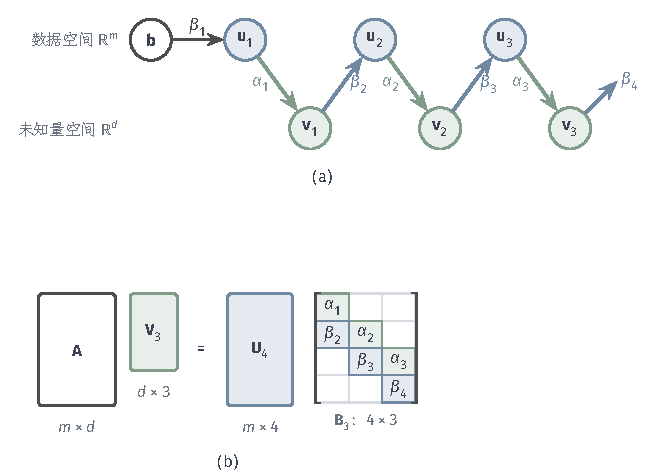
\includegraphics[width=109.343mm]{figures/01-basic-mathematics/03-vectors-matrices-and-multivariate-functions/tikz/c5-golub-kahan-bidiagonal/figure.pdf}
  \caption{Golub--Kahan双对角化的递推与矩阵关系（$k=3$）。(a)蓝色$\bm u_i$在数据空间，绿色$\bm v_i$在未知量空间；乘$\bm A^\top$并扣除前一个$\bm v$后归一化得到$\bm v_i$，长度为$\alpha_i$，乘$\bm A$并扣除前一个$\bm u$后归一化得到$\bm u_{i+1}$，长度为$\beta_{i+1}$。(b)这些长度排成$4\times3$的下双对角矩阵$\bm B_3$，满足$\bm A\bm V_3=\bm U_4\bm B_3$；绿格为对角元，蓝格为次对角元，其余元素为零。}
  \label{fig:ls-golub-kahan-bidiagonal}
\end{figure}

\paragraph{数值敏感度}
在浮点运算中，正交性所依赖的相消只近似成立，短递推也不会去掉舍入引入的旧方向分量，两组基会逐渐失去正交性；它对求解结果的影响交给两种求解器，由求解器在停止前的真实残差复核来控制，必要时以保存基并重正交化的代价换取正交性。

\paragraph{计算代价}
每轮至多一次$\bm A$乘向量和一次$\bm A^\top$乘向量，外加两次向量更新、两次范数和两次缩放。调用者只用当前的$\bm u_k,\bm v_k$，不保存整组基、不作完整再正交化时，工作存储为$O(m+d)$，与Lanczos过程一样不随轮数增长。双对角化只负责生成候选空间，收敛快慢取决于求解器在子空间中怎样选取近似解。

\subsection{应用}
\label{sec:ls-golub-kahan-application}

有了两组基与双对角矩阵，就可以在子空间中求解最小二乘问题。零初值下把近似写成
\[
 \bm x=\bm V_k\bm y ,
\]
$\bm y\in\mathbb R^k$是$\mathcal K_k(\bm A^\top\bm A,\bm A^\top\bm b)$中的坐标。

由$\bm b=\beta_1\bm u_1=\bm U_{k+1}\beta_1\bm e_1$与关系~\eqref{eq:ls-golub-kahan-relations}的第一式，
\begin{equation}
 \bm b-\bm A\bm V_k\bm y=\bm U_{k+1}\bigl(\beta_1\bm e_1-\bm B_k\bm y\bigr).
 \label{eq:ls-golub-kahan-residual-coordinates}
\end{equation}
$\bm U_{k+1}$的列标准正交，不改变长度，所以在子空间中使原残差最小，化为$(k+1)\times k$的双对角最小二乘问题
\begin{equation}
 \min_{\bm y}\lVert\beta_1\bm e_1-\bm B_k\bm y\rVert_2 .
 \label{eq:ls-golub-kahan-lsqr-problem}
\end{equation}
这就是LSQR（第~\ref{sec:ls-lsqr}节）的做法；$\bm B_k$每增加一列只在右下角多出两个非零元，一次新的正交变换就能延续三角化，解可以由短递推逐步累加。

若改为使正规残差最小，再用关系~\eqref{eq:ls-golub-kahan-relations}的第二式把$\bm A^\top$作用上去。$\bm B_k$的首行是$\alpha_1\bm e_1^\top$、末行是$\beta_{k+1}\bm e_k^\top$，于是
\begin{equation}
 \bm A^\top\bigl(\bm b-\bm A\bm V_k\bm y\bigr)
 =\bm V_k\bigl(\alpha_1\beta_1\bm e_1-\bm B_k^\top\bm B_k\bm y\bigr)-\alpha_{k+1}\beta_{k+1}y_k\bm v_{k+1},
 \label{eq:ls-golub-kahan-normal-residual-coordinates}
\end{equation}
其中$y_k$是$\bm y$的末分量。右端仍由标准正交的$\bm v_1,\ldots,\bm v_{k+1}$表示，正规残差的长度因此也化为关于三对角矩阵$\bm B_k^\top\bm B_k$及一个边界项的小问题。这就是LSMR（第~\ref{sec:ls-lsmr}节）的做法，它实际计算时并不形成$\bm B_k^\top\bm B_k$。

两者的子空间、两组基和双对角矩阵都来自同一个双对角化，区别只在于最小化原残差还是正规残差。它们与方阵情形的对应也很清楚：对正规方程而言，LSQR相当于在Lanczos基上用Galerkin条件，LSMR相当于极小残差条件，第~\ref{sec:ls-lsqr}节与第~\ref{sec:ls-lsmr}节将分别证明它们与正规方程上的CG和MINRES等价。

\section{最小残差法}
\label{sec:ls-minres}

设$\bm A$实对称非奇异，允许不定。这时$\bm u^\top\bm A\bm u$可以为负，误差的能量范数没有定义，原残差长度却始终有意义。\term{最小残差法}（minimal residual method，MINRES）在第$k$步取$\bm x_0+\mathcal K_k$中使$\lVert\bm b-\bm A\bm x\rVert_2$最小的近似，即第~\ref{sec:ls-krylov-selection-criteria}节的极小残差条件。

它紧接第~\ref{sec:ls-lanczos-application}节的应用：Lanczos过程（递推~\eqref{eq:ls-lanczos-step}）已经给出$\mathcal K_k$的标准正交基$\bm V_k$与三对角矩阵$\overline{\bm T}_k$，并把问题化为$(k+1)\times k$的小型最小二乘问题；对称不定时$\bm T_k$可能奇异，所以不解Galerkin方程~\eqref{eq:ls-lanczos-projected-system}，而在这个小问题上求残差最小的坐标。本节说明怎样随Lanczos过程逐列求解它，使每轮的工作量与存储都不随步数增长。

\subsection{主要思想}

\paragraph{逐步长大的小问题}
把候选写成$\bm x=\bm x_0+\bm V_k\bm y$，$\bm y\in\mathbb R^k$是子空间中的坐标。记$\beta=\lVert\bm r_0\rVert_2$，则$\bm r_0=\beta\bm V_{k+1}\bm e_1$，由关系~\eqref{eq:ls-arnoldi-tridiagonal}，
\[
 \bm b-\bm A\bm x=\bm r_0-\bm A\bm V_k\bm y=\bm V_{k+1}(\beta\bm e_1-\overline{\bm T}_k\bm y).
\]
定理~\ref{thm:ls-arnoldi-lanczos}保证$\bm V_{k+1}$的列标准正交，不改变长度，于是
\begin{equation}
 \lVert\bm b-\bm A\bm x\rVert_2=\lVert\beta\bm e_1-\overline{\bm T}_k\bm y\rVert_2 .
 \label{eq:ls-minres-small-problem}
\end{equation}
MINRES在每一步都要求出使右端最小的$\bm y$。

这个小问题随步数长大。第$k$步的$(k+1)\times k$矩阵是
\[
 \overline{\bm T}_k=
 \begin{bmatrix}
 a_1&\gamma_1&&&\\
 \gamma_1&a_2&\gamma_2&&\\
 &\gamma_2&a_3&\ddots&\\
 &&\ddots&\ddots&\gamma_{k-1}\\
 &&&\gamma_{k-1}&a_k\\
 &&&&\gamma_k
 \end{bmatrix}.
\]
从第$k-1$步到第$k$步，Lanczos过程只多算出一对系数$a_k,\gamma_k$，矩阵只在右侧添了一列、在下方添了一行：新的一列是$(0,\ldots,0,\gamma_{k-1},a_k,\gamma_k)^\top$，只有最后三个元素非零；新的一行只有末元素$\gamma_k$。

如果每一步都对整个$\overline{\bm T}_k$重新作一次QR分解，工作量会随$k$增长，而且要保存全部基向量才能还原解。但矩阵每步只变了这么一点，前一步的分解结果完全可以沿用，只需处理新增的部分。下面说明这种增量求解怎样进行。

\paragraph{沿用前一步的消元结果}
小问题按第~\ref{sec:ls-qr-method}节的思路用Givens旋转化为上三角。第$j$个旋转$\bm G_j$只作用于第$j$、$j+1$两行，在这两行上的形式为
\begin{equation}
 \begin{bmatrix}c_j&s_j\\-s_j&c_j\end{bmatrix},\qquad c_j^2+s_j^2=1 .
 \label{eq:ls-minres-givens}
\end{equation}
设前$k-1$步已经用$\bm G_1,\ldots,\bm G_{k-1}$把$\overline{\bm T}_{k-1}$消成了上三角。由于$\overline{\bm T}_{k-1}$是三对角的，所得上三角矩阵每列至多三个非零元，记第$j$列为$\epsilon_j,\delta_j,\rho_j$，位于第$j-2,j-1,j$行。以$k=4$为例，前三列经过$\bm G_1,\bm G_2,\bm G_3$后成为
\[
 \begin{bmatrix}
 \rho_1&\delta_2&\epsilon_3\\
 0&\rho_2&\delta_3\\
 0&0&\rho_3\\
 0&0&0
 \end{bmatrix}.
\]
以后的旋转只作用于第$4$行及以下，这三列不再改变。

\paragraph{新列只需三次旋转}
第$k$步添入的新列只在第$k-1$、$k$、$k+1$行非零。依次把旧旋转作用上去：$\bm G_1,\ldots,\bm G_{k-3}$作用的行在新列中都是零，不起作用；真正改变新列的只有最后两个旧旋转$\bm G_{k-2}$与$\bm G_{k-1}$。之后，新列最下方还剩一个非零元$\gamma_k$，再构造一个新旋转$\bm G_k$把它消去。

仍以$k=4$为例，新列是$(0,0,\gamma_3,a_4,\gamma_4)^\top$，逐次旋转的变化为
\[
 \begin{bmatrix}0\\0\\\gamma_3\\a_4\\\gamma_4\end{bmatrix}
 \xrightarrow{\ \bm G_2\ }
 \begin{bmatrix}0\\\epsilon_4\\\theta\\a_4\\\gamma_4\end{bmatrix}
 \xrightarrow{\ \bm G_3\ }
 \begin{bmatrix}0\\\epsilon_4\\\delta_4\\\bar\delta\\\gamma_4\end{bmatrix}
 \xrightarrow{\ \bm G_4\ }
 \begin{bmatrix}0\\\epsilon_4\\\delta_4\\\rho_4\\0\end{bmatrix}.
\]
$\bm G_1$作用于第$1$、$2$行，那里都是零，所以没有画出。整个矩阵在新旋转之前与之后分别是
\[
 \begin{bmatrix}
 \rho_1&\delta_2&\epsilon_3&0\\
 0&\rho_2&\delta_3&\epsilon_4\\
 0&0&\rho_3&\delta_4\\
 0&0&0&\bar\delta\\
 0&0&0&\gamma_4
 \end{bmatrix}
 \xrightarrow{\ \bm G_4\ }
 \begin{bmatrix}
 \rho_1&\delta_2&\epsilon_3&0\\
 0&\rho_2&\delta_3&\epsilon_4\\
 0&0&\rho_3&\delta_4\\
 0&0&0&\rho_4\\
 0&0&0&0
 \end{bmatrix}.
\]
只有右下角的$\bar\delta$与$\gamma_4$需要新旋转处理，其余元素都沿用上一步的结果。

一般地，把每个$2\times2$旋转分别作用于新列的相应两个分量，就得到第$j$步的计算公式：
\begin{equation}
 \begin{gathered}
 \epsilon_j=s_{j-2}\gamma_{j-1},\qquad \theta=c_{j-2}\gamma_{j-1},\\
 \delta_j=c_{j-1}\theta+s_{j-1}a_j,\qquad
 \bar\delta=-s_{j-1}\theta+c_{j-1}a_j,\\
 \rho_j=\sqrt{\bar\delta^2+\gamma_j^2},\qquad
 c_j=\bar\delta/\rho_j,\qquad s_j=\gamma_j/\rho_j .
 \end{gathered}
 \label{eq:ls-minres-rotation}
\end{equation}
第一行是$\bm G_{j-2}$作用于$(0,\gamma_{j-1})$，第二行是$\bm G_{j-1}$作用于$(\theta,a_j)$，第三行选取$c_j,s_j$使$\bm G_j$把$(\bar\delta,\gamma_j)$变成$(\rho_j,0)$。前两步尚不存在的旧旋转取单位变换$(c,s)=(1,0)$。

\paragraph{右端与残差}
同一组旋转也作用于右端$\beta\bm e_1$。它的第$j+1$个分量起初为零，只有第$j$个旋转才把非零值带下来。把第$j$个分量在$\bm G_j$作用之前的值记为$\bar g_j$，$\bar g_1=\beta$，则
\begin{equation}
 g_j=c_j\bar g_j,\qquad \bar g_{j+1}=-s_j\bar g_j .
 \label{eq:ls-minres-rhs}
\end{equation}
以$k=4$为例，右端在$\bm G_4$前后分别是
\[
 \begin{bmatrix}g_1\\g_2\\g_3\\\bar g_4\\0\end{bmatrix}
 \xrightarrow{\ \bm G_4\ }
 \begin{bmatrix}g_1\\g_2\\g_3\\g_4\\\bar g_5\end{bmatrix}.
\]
旋转不改变长度，旋转后的小问题是使
\[
 \bigl\lVert(g_1,\ldots,g_k,\bar g_{k+1})^\top-[\bm R_k;\bm 0]\bm y\bigr\rVert_2
\]
最小。前$k$个方程可由上三角的$\bm R_k$精确满足，最后一个分量$\bar g_{k+1}$无论$\bm y$取什么都无法消去，所以最小残差长度就是
\begin{equation}
 \min_{\bm y}\lVert\beta\bm e_1-\overline{\bm T}_k\bm y\rVert_2=\lvert\bar g_{k+1}\rvert .
 \label{eq:ls-minres-residual-estimate}
\end{equation}

\paragraph{增量求解的两个好处}
其一，每步的工作量固定。第$j$步只作用两个旧旋转、构造一个新旋转、更新右端的两个分量，都是几个标量运算，不随$j$增长；加上一次Lanczos递推与下面的向量更新，每步的工作量与存储都与步数无关。

其二，残差长度随消元一起得到。精确算术下$\lvert\bar g_{k+1}\rvert$就是第$k$步近似的原残差长度$\lVert\bm b-\bm A\bm x_k\rVert_2$，每步只需一次乘法即可读出，不必形成近似解；又因$\lvert s_j\rvert\le1$，它随步数不增。浮点计算中它会逐渐偏离真实残差，所以最终仍要用$\bm b-\bm A\bm x$复核。

\paragraph{方向与解的短递推}
最小点满足$\bm R_k\bm y=(g_1,\ldots,g_k)^\top$，直接回代需要保存全部基向量才能还原$\bm x$。改为在原空间中累加：令$\bm D_k=\bm V_k\bm R_k^{-1}$，比较$\bm D_k\bm R_k=\bm V_k$的第$j$列，
\[
 \bm v_j=\epsilon_j\bm d_{j-2}+\delta_j\bm d_{j-1}+\rho_j\bm d_j ,
\]
解出
\begin{equation}
 \bm d_j=\frac{\bm v_j-\delta_j\bm d_{j-1}-\epsilon_j\bm d_{j-2}}{\rho_j} ,
 \label{eq:ls-minres-direction}
\end{equation}
约定$\bm d_{-1}=\bm d_0=\bm 0$。由于$\bm R_k$的旧列与已确定的$g_j$以后都不再改变，近似解可以逐项累加：
\begin{equation}
 \bm x_j=\bm x_{j-1}+g_j\bm d_j .
 \label{eq:ls-minres-update}
\end{equation}
每步只需保留两个旧方向和两个旧旋转。定理~\ref{thm:ls-minres-optimality}说明，这样累加得到的$\bm x_k$正是小问题~\eqref{eq:ls-minres-small-problem}的解所对应的近似。

\subsection{算法实现}

每轮作一步Lanczos递推得到$\overline{\bm T}_k$的新列，用两个旧旋转与一个新旋转消元，再更新右端、方向与解。输入为实对称非奇异矩阵$\bm A$与右端$\bm b$，算法只需计算$\bm A$乘向量；预先选定的参数与第~\ref{sec:ls-matrix-splitting}节执行流程相同：初值$\bm x_0$、容差$\mathrm{atol},\mathrm{rtol}$与最大轮数$K$，停止检查沿用该流程的阈值$\tau$。下面写出计算中用到的变量、它们怎样初始化、每轮怎样更新。下面用例~\ref{ex:ls-stationary-running-example}的以下数据逐步演示：
\[
 \bm A=\begin{bmatrix}4&1\\1&3\end{bmatrix},\qquad \bm b=\begin{bmatrix}1\\2\end{bmatrix}.
\]
取$\bm x_0=\bm 0$，精确解为$\bm x_\star=(1/11,7/11)^\top$。Lanczos部分的数值与第~\ref{sec:ls-lanczos}节相同。

\paragraph{变量}
\begin{itemize}
 \item $\bm v_{j-1},\bm v_j\in\mathbb R^d$：上一个与当前Lanczos基向量；$\bm w\in\mathbb R^d$：工作向量，存放扣除后的余项。
 \item $a_j,\gamma_j$：$\overline{\bm T}_k$第$j$列的对角元与次对角元；$\gamma_{j-1}$留到本轮使用。
 \item $(c_{j-2},s_{j-2}),(c_{j-1},s_{j-1})$：两个旧旋转；$(c_j,s_j)$：本轮的新旋转。
 \item $\epsilon_j,\delta_j,\rho_j$：$\bm R_k$第$j$列的三个非零元；$\theta,\bar\delta$：旋转过程中的临时量。
 \item $\bar g_j$：右端第$j$个分量旋转前的值，旋转后得到$g_j$与$\bar g_{j+1}$；$\lvert\bar g_{j+1}\rvert$是第$j$步的残差长度。
 \item $\bm d_{j-2},\bm d_{j-1},\bm d_j\in\mathbb R^d$：两个旧方向与当前方向。
 \item $\bm x_j\in\mathbb R^d$：当前近似解，在原处更新。
 \item $j$：轮次。
\end{itemize}

\paragraph{初始化}
先计算$\bm r_0=\bm b-\bm A\bm x_0$并作停止检查，已达标则直接输出$\bm x_0$。否则按Lanczos过程初始化基向量，把方向初始化为零向量，右端初始化为$\beta$，两个尚不存在的旧旋转初始化为单位变换，轮次初始化为$1$：
\[
 \begin{gathered}
 \beta=\lVert\bm r_0\rVert_2,\qquad \bm v_0=\bm 0,\qquad \bm v_1=\frac{\bm r_0}{\beta},\qquad \gamma_0=0,\\
 \bm d_{-1}=\bm d_0=\bm 0,\qquad \bar g_1=\beta,\\
 (c_{-1},s_{-1})=(c_0,s_0)=(1,0),\qquad j=1 .
 \end{gathered}
\]
例中$\bm r_0=\bm b$，
\[
 \beta=\sqrt5,\qquad \bm v_1=\frac1{\sqrt5}\begin{bmatrix}1\\2\end{bmatrix},\qquad \bar g_1=\sqrt5 .
\]

\paragraph{每轮更新}
在第$j$轮：
\begin{enumerate}
 \item \textbf{Lanczos递推。}按式~\eqref{eq:ls-lanczos-step}计算
 \[
  \begin{gathered}
  a_j=\bm v_j^\top\bm A\bm v_j,\\
  \bm w=\bm A\bm v_j-a_j\bm v_j-\gamma_{j-1}\bm v_{j-1},\qquad \gamma_j=\lVert\bm w\rVert_2 ,
  \end{gathered}
 \]
 得到$\overline{\bm T}_k$的第$j$列$(\gamma_{j-1},a_j,\gamma_j)^\top$；归一化留到第5步。
 例中第一轮
 \[
  a_1=4,\qquad \bm w=\frac1{\sqrt5}\begin{bmatrix}2\\-1\end{bmatrix},\qquad \gamma_1=1 ,
 \]
 第一列为$(0,4,1)^\top$。

 \item \textbf{旋转消元。}按式~\eqref{eq:ls-minres-rotation}依次用第$j-2$、$j-1$个旋转处理这一列，再构造新旋转，得到$\epsilon_j,\delta_j,\rho_j$与$c_j,s_j$。$\bm A$非奇异时$\overline{\bm T}_k$满列秩，正常步骤中$\rho_j>0$；若出现$\rho_j=0$，不执行除法，先检查小问题的秩与相容性。
 例中第一轮两个旧旋转都是单位变换，$\epsilon_1=\delta_1=0$，$\bar\delta=a_1=4$，
 \[
  \rho_1=\sqrt{17},\qquad c_1=\frac4{\sqrt{17}},\qquad s_1=\frac1{\sqrt{17}} .
 \]

 \item \textbf{更新右端。}按式~\eqref{eq:ls-minres-rhs}计算
 \[
  g_j=c_j\bar g_j,\qquad \bar g_{j+1}=-s_j\bar g_j .
 \]
 例中第一轮
 \[
  g_1=\frac{4\sqrt5}{\sqrt{17}},\qquad \bar g_2=-\frac{\sqrt5}{\sqrt{17}},\qquad \lvert\bar g_2\rvert=\sqrt{\frac5{17}}\approx0.542 .
 \]

 \item \textbf{更新方向与解。}按式~\eqref{eq:ls-minres-direction}与式~\eqref{eq:ls-minres-update}计算
 \[
  \bm d_j=\frac{\bm v_j-\delta_j\bm d_{j-1}-\epsilon_j\bm d_{j-2}}{\rho_j},\qquad
  \bm x_j=\bm x_{j-1}+g_j\bm d_j ,
 \]
 然后舍去$\bm d_{j-2}$与第$j-2$个旋转。
 例中第一轮
 \[
  \bm d_1=\frac{\bm v_1}{\rho_1}=\frac1{\sqrt{85}}\begin{bmatrix}1\\2\end{bmatrix},\qquad
  \bm x_1=g_1\bm d_1=\frac1{17}\begin{bmatrix}4\\8\end{bmatrix}.
 \]
 可以核对$\bm b-\bm A\bm x_1=(-7,6)^\top/17$，长度正是$\lvert\bar g_2\rvert=\sqrt{5/17}$。

 第一轮不满足第5步的停止条件，令$\bm v_2=\bm w/\gamma_1=(2,-1)^\top/\sqrt5$，进入第二轮。由第1步，
 \[
  a_2=3,\qquad \bm w=\bm 0,\qquad \gamma_2=0 ,
 \]
 第二列为$(1,3,0)^\top$。由第2步，先用第$0$个旋转得
 \[
  \epsilon_2=s_0\gamma_1=0,\qquad \theta=c_0\gamma_1=1 ,
 \]
 再用第$1$个旋转并构造新旋转，得
 \[
  \begin{gathered}
  \delta_2=\frac7{\sqrt{17}},\qquad \bar\delta=\frac{11}{\sqrt{17}},\qquad \rho_2=\frac{11}{\sqrt{17}},\\
  c_2=1,\qquad s_2=0 .
  \end{gathered}
 \]
 由第3步，
 \[
  g_2=-\frac{\sqrt5}{\sqrt{17}},\qquad \bar g_3=0 .
 \]
 由第4步，新方向为
 \[
  \bm d_2=\frac1{11\sqrt{85}}\begin{bmatrix}27\\-31\end{bmatrix},
 \]
 近似解更新为
 \[
  \bm x_2=\frac1{17}\begin{bmatrix}4\\8\end{bmatrix}-\frac1{187}\begin{bmatrix}27\\-31\end{bmatrix}=\frac1{11}\begin{bmatrix}1\\7\end{bmatrix}.
 \]

 \item \textbf{停止。}若残差估计$\lvert\bar g_{j+1}\rvert\le\tau$，或$\gamma_j=0$（子空间不再扩张，此时$s_j=0$，$\bar g_{j+1}=0$），或$j=K$，就用$\bm b-\bm A\bm x_j$复核真实残差后输出$\bm x_j$，并按第~\ref{sec:ls-stationary-stopping}节报告结束原因；否则令$\bm v_{j+1}=\bm w/\gamma_j$、$j\leftarrow j+1$，回到第1步。
 例中第一轮$\lvert\bar g_2\rvert\approx0.542$未达标，且$\gamma_1\ne0$，继续迭代；第二轮$\bar g_3=0$且$\gamma_2=0$，复核得真实残差为零，以“达到容差”退出迭代。
\end{enumerate}

最终得到近似解$\bm x_2$，它就是小问题~\eqref{eq:ls-minres-small-problem}的最小点所对应的近似。例中两个旋转把$\overline{\bm T}_2$化为
\[
 \bm R_2=\frac1{\sqrt{17}}\begin{bmatrix}17&7\\0&11\end{bmatrix},
\]
回代$\bm R_2\bm y=(g_1,g_2)^\top$得
\[
 \bm y=(3\sqrt5,-\sqrt5)^\top/11 ,
\]
于是
\[
 \bm x_2=\bm x_0+\bm V_2\bm y=\frac1{11}\begin{bmatrix}1\\7\end{bmatrix}=\bm x_\star ,
\]
与短递推的结果一致；代回得$\bm A\bm x_2=(11,22)^\top/11=\bm b$。

二维问题在第二轮子空间用尽，最小残差为零，MINRES给出精确解。

贯穿例是正定的。下面换用对称不定矩阵，这时能量范数没有定义，下一节的CG也因此不适用，MINRES仍然可用。

\begin{example}[对称不定矩阵上的MINRES]
\label{ex:ls-minres-indefinite}
取$\bm A=\operatorname{diag}(1,-2)$，$\bm b=(1,1)^\top$，$\bm x_0=\bm0$。$\bm A$有一个正特征值和一个负特征值；例如$\bm b^\top\bm A\bm b=1-2=-1<0$，$\bm u^\top\bm A\bm u$不能作为范数的平方。MINRES只需要对称性。

初始化得$\beta=\sqrt2$，$\bm v_1=(1,1)^\top/\sqrt2$。

第一轮由式~\eqref{eq:ls-lanczos-step}，先算出
\[
 \bm A\bm v_1=(1,-2)^\top/\sqrt2 ,
\]
再得
\[
 a_1=-\frac12,\qquad \gamma_1=\frac32,\qquad \bm v_2=\frac1{\sqrt2}\begin{bmatrix}1\\-1\end{bmatrix}.
\]
没有旧旋转，由式~\eqref{eq:ls-minres-rotation}与\eqref{eq:ls-minres-rhs}，
\[
 \begin{gathered}
 \rho_1=\frac{\sqrt{10}}2,\qquad c_1=-\frac1{\sqrt{10}},\qquad s_1=\frac3{\sqrt{10}},\\
 g_1=-\frac1{\sqrt5},\qquad \bar g_2=-\frac3{\sqrt5} .
 \end{gathered}
\]
于是
\[
 \bm d_1=\bm v_1/\rho_1=(1,1)^\top/\sqrt5,\qquad \bm x_1=g_1\bm d_1=(-1/5,-1/5)^\top .
\]
直接计算
\[
 \bm r_1=\bm b-\bm A\bm x_1=(6/5,3/5)^\top ,
\]
长度$3/\sqrt5=\lvert\bar g_2\rvert$。

第二轮先作Lanczos递推，
\[
 \bm w=\bm A\bm v_2-\gamma_1\bm v_1=(-1/2,1/2)^\top/\sqrt2,\qquad a_2=-1/2 ,
\]
扣除后余项为零，$\gamma_2=0$，第二列为$(3/2,-1/2,0)^\top$。

旋转给出$\epsilon_2=0$、$\theta=3/2$，以及
\[
 \begin{gathered}
 \delta_2=-\frac3{\sqrt{10}},\qquad \bar\delta=-\frac4{\sqrt{10}},\qquad \rho_2=\frac4{\sqrt{10}},\\
 c_2=-1,\qquad s_2=0 ,
 \end{gathered}
\]
于是
\[
 g_2=c_2\bar g_2=3/\sqrt5,\qquad \bar g_3=0 .
\]
由式~\eqref{eq:ls-minres-direction}与\eqref{eq:ls-minres-update}，
\[
 \bm d_2=\frac1{\sqrt5}\begin{bmatrix}2\\-\tfrac12\end{bmatrix},\qquad
 \bm x_2=\bm x_1+g_2\bm d_2=\begin{bmatrix}1\\-\tfrac12\end{bmatrix},
\]
代回得$\bm A\bm x_2=(1,1)^\top=\bm b$。

再独立核验。两轮的系数组成
\[
 \bm T_2=\begin{bmatrix}-1/2&3/2\\3/2&-1/2\end{bmatrix},
\]
直接解小问题$\bm T_2\bm y=\beta\bm e_1$得
\[
 \bm y=(\sqrt2/4,3\sqrt2/4)^\top ,
\]
而$\bm V_2\bm y=(1,-1/2)^\top$，与短递推的结果一致。
\end{example}

\subsection{算法分析}

\paragraph{正确性}
正确性归结为两点：小问题~\eqref{eq:ls-minres-small-problem}与原问题等价，旋转与短递推给出小问题的解。

\begin{theorem}[MINRES的最小残差性]
\label{thm:ls-minres-optimality}
设$\bm A$实对称非奇异，在精确算术下执行MINRES至第$k$步，且此前的$\gamma_1,\ldots,\gamma_{k-1}$均非零。则$\bm x_k$是残差长度在$\bm x_0+\mathcal K_k$上的唯一最小点；$\lVert\bm r_k\rVert_2=\lvert\bar g_{k+1}\rvert$随$k$不增，MINRES至多$d$步得到精确解，并且
\begin{equation}
 \lVert\bm r_k\rVert_2\le\min_{p\in\mathcal P_k}\max_{\lambda\in\sigma(\bm A)}\lvert p(\lambda)\rvert\,\lVert\bm r_0\rVert_2 ,
 \label{eq:ls-minres-residual-bound}
\end{equation}
其中$\mathcal P_k$同引理~\ref{lem:ls-krylov-residual-polynomial}。
\end{theorem}

\begin{proof}
证明分三步：先把原问题化为小问题，再说明旋转与短递推给出小问题的解，最后由残差多项式得到界。

\emph{化为小问题。}由Lanczos关系（定理~\ref{thm:ls-arnoldi-lanczos}），递推~\eqref{eq:ls-lanczos-step}给出的$\bm V_{k+1}$列标准正交，$\bm V_k$张成$\mathcal K_k$，并且关系~\eqref{eq:ls-arnoldi-tridiagonal}成立；$\gamma_k=0$时$\overline{\bm T}_k$的末行为零，略去它与$\bm v_{k+1}$后下面的推导照样成立。由$\bm r_0=\beta\bm V_{k+1}\bm e_1$，
\[
 \bm b-\bm A(\bm x_0+\bm V_k\bm y)=\bm r_0-\bm A\bm V_k\bm y=\bm V_{k+1}(\beta\bm e_1-\overline{\bm T}_k\bm y),
\]
$\bm V_{k+1}$的列标准正交，不改变长度，即得式~\eqref{eq:ls-minres-small-problem}。$\bm V_k$满列秩，$\bm y\mapsto\bm x_0+\bm V_k\bm y$是$\mathbb R^k$到$\bm x_0+\mathcal K_k$的双射，两个最小化问题的解一一对应。

\emph{旋转与短递推。}$\overline{\bm T}_k$第$j$列的非零元在第$j-1,j,j+1$行，第$i$个旋转只作用于第$i,i+1$行，所以$i<j-2$的旋转碰到的都是零，只有第$j-2$、$j-1$个起作用，乘出来就是式~\eqref{eq:ls-minres-rotation}，$\bm R_k$的上带宽为$2$。记$k$个旋转之积为正交矩阵$\bm\Omega_k$，则
\[
 \bm\Omega_k\overline{\bm T}_k=\begin{bmatrix}\bm R_k\\\bm 0^\top\end{bmatrix},\qquad
 \bm\Omega_k\beta\bm e_1=(g_1,\ldots,g_k,\bar g_{k+1})^\top ,
\]
从而
\[
 \lVert\beta\bm e_1-\overline{\bm T}_k\bm y\rVert_2^2=\lVert(g_1,\ldots,g_k)^\top-\bm R_k\bm y\rVert_2^2+\bar g_{k+1}^2 .
\]
$\bm A$非奇异且$\bm V_k$满列秩，$\bm A\bm V_k=\bm V_{k+1}\overline{\bm T}_k$满列秩，故$\overline{\bm T}_k$与$\bm R_k$满秩，$\bm R_k$可逆。唯一最小点是$\bm y=\bm R_k^{-1}(g_1,\ldots,g_k)^\top$，最小值为$\lvert\bar g_{k+1}\rvert$。令$\bm D_k=\bm V_k\bm R_k^{-1}$，比较$\bm D_k\bm R_k=\bm V_k$的第$j$列，
\[
 \bm v_j=\epsilon_j\bm d_{j-2}+\delta_j\bm d_{j-1}+\rho_j\bm d_j ,
\]
解出即式~\eqref{eq:ls-minres-direction}。于是
\[
 \bm x_k=\bm x_0+\bm V_k\bm R_k^{-1}(g_1,\ldots,g_k)^\top=\bm x_0+\sum_{j\le k}g_j\bm d_j .
\]
后来的旋转只作用于更靠后的行，已确定的$g_j$与$\bm R_k$已有的列不再改变，所以逐步累加~\eqref{eq:ls-minres-update}得到的正是这个最小点。

\emph{单调性与有限步终止。}由式~\eqref{eq:ls-minres-rhs}，
\[
 \lvert\bar g_{k+1}\rvert=\lvert s_k\rvert\,\lvert\bar g_k\rvert\le\lvert\bar g_k\rvert ,
\]
残差长度不增。若$\gamma_k=0$，则$s_k=0$，$\bar g_{k+1}=0$，残差为零；子空间维数不超过$d$，所以至多$d$步出现这一情形或零残差。

\emph{残差界。}由引理~\ref{lem:ls-krylov-residual-polynomial}与最小残差性，
\[
 \lVert\bm r_k\rVert_2=\min_{p\in\mathcal P_k}\lVert p(\bm A)\bm r_0\rVert_2 .
\]
由谱定理（定理~\ref{thm:ls-real-symmetric-spectral}），$\bm A=\bm Q\bm\Lambda\bm Q^\top$，$\bm Q$正交，于是$p(\bm A)=\bm Q\,p(\bm\Lambda)\bm Q^\top$，
\[
 \lVert p(\bm A)\bm r_0\rVert_2\le\lVert p(\bm\Lambda)\rVert_2\lVert\bm r_0\rVert_2=\max_{\lambda\in\sigma(\bm A)}\lvert p(\lambda)\rvert\,\lVert\bm r_0\rVert_2 ,
\]
对$p$取最小即得所述界。
\end{proof}

第~\ref{sec:ls-gmres}节的GMRES对一般方阵采用同一准则；$\bm A$对称时两者的近似相同，MINRES只是借助对称性改用短递推。

\paragraph{收敛速度}
界中只剩特征值，收敛快慢完全由谱决定。不定时特征值分布在原点两侧，而多项式在原点必须取$1$，要同时压低两侧谱上的值，比只压低一侧更难。

\paragraph{奇异系统的边界}
本节的结论假定$\bm A$非奇异。若把MINRES用于奇异对称矩阵，不相容时最小残差不为零，判断是否到达最小二乘解要看$\lVert\bm A\bm r_k\rVert_2$是否足够小，而不是看$\lVert\bm r_k\rVert_2$；即使到达，普通MINRES给出的最小残差解也不自动具有最小欧氏范数。这里不展开奇异对称系统的专门算法（如MINRES-QLP）。

\paragraph{数值敏感度与计算代价}
浮点计算中，Lanczos向量会逐渐失去正交性，原因见第~\ref{sec:ls-lanczos}节。因此残差估计$\lvert\bar g_{j+1}\rvert$须用真实残差复核。每轮核心递推需要一次$\bm A$乘向量，只保存$\bm v_{j-1},\bm v_j,\bm w,\bm d_{j-2},\bm d_{j-1},\bm x$等固定数量的向量，存储不随步数增长，而保存全部基的GMRES执行$k$步需要约$kd$个数；若为保持正交性作完整的再正交化，就要保存全部基，存储同样随步数增长。

\section{共轭梯度法}
\label{sec:ls-conjugate-gradient}

设$\bm A=\bm A^\top\succ0$。\term{共轭梯度法}（conjugate gradient method，CG）在第$k$步取$\bm x_0+\mathcal K_k$中使误差的能量范数
\[
 \lVert\bm x-\bm x_\star\rVert_{\bm A}=\bigl((\bm x-\bm x_\star)^\top\bm A(\bm x-\bm x_\star)\bigr)^{1/2}
\]
最小的近似，这等价于第~\ref{sec:ls-krylov-selection-criteria}节的Galerkin条件。

它紧接第~\ref{sec:ls-lanczos-application}节的应用：那里在Lanczos基下把Galerkin条件化成了三对角方程，CG就是对称正定时求解这个方程的一种特殊做法。

\subsection{主要思想}
\label{sec:ls-cg-derivation}

\paragraph{逐步长大的三对角方程}
由第~\ref{sec:ls-lanczos-application}节，把近似写成$\bm x_k=\bm x_0+\bm V_k\bm y_k$后，Galerkin条件给出三对角方程~\eqref{eq:ls-lanczos-projected-system}：
\[
 \bm T_k\bm y_k=\lVert\bm r_0\rVert_2\,\bm e_1,\qquad
 \bm T_k=
 \begin{bmatrix}
 a_1&\gamma_1&&\\
 \gamma_1&a_2&\ddots&\\
 &\ddots&\ddots&\gamma_{k-1}\\
 &&\gamma_{k-1}&a_k
 \end{bmatrix}.
\]
与MINRES一样，$k$每增加$1$，$\bm T_k$只在右侧添一列、在下方添一行，新添的元素只有$\gamma_{k-1}$（两次）与$a_k$。不同的是，这里$\bm A$对称正定，$\bm T_k=\bm V_k^\top\bm A\bm V_k$也对称正定，要解的是一个方阵方程，而不是最小二乘问题。

MINRES面对的$\overline{\bm T}_k$可能来自不定矩阵，要用Givens旋转作QR分解，才能稳妥地处理正负特征值。对称正定的$\bm T_k$可以走更直接的路：作第~\ref{sec:ls-cholesky}节Cholesky分解的无开方形式，即$\bm L\bm D\bm L^\top$分解，而且不必选主元。下面说明这个分解怎样随步数延伸，再把它翻译回向量，得到CG的短递推。

\paragraph{分解的增量更新}
把$\bm T_k$分解为
\begin{equation}
 \bm T_k=\bm L_k\bm D_k\bm L_k^\top ,
 \label{eq:ls-cg-tridiagonal-ldl}
\end{equation}
其中$\bm L_k$是单位下双对角矩阵，次对角元记为$\ell_1,\ldots,\ell_{k-1}$；$\bm D_k$是对角矩阵，对角元记为$d_1,\ldots,d_k$。以$k=3$为例，
\[
 \begin{aligned}
 \bm L_3\bm D_3\bm L_3^\top
 &=\begin{bmatrix}1&&\\\ell_1&1&\\&\ell_2&1\end{bmatrix}
 \begin{bmatrix}d_1&&\\&d_2&\\&&d_3\end{bmatrix}
 \begin{bmatrix}1&\ell_1&\\&1&\ell_2\\&&1\end{bmatrix}\\
 &=\begin{bmatrix}d_1&\ell_1d_1&\\\ell_1d_1&\ell_1^2d_1+d_2&\ell_2d_2\\&\ell_2d_2&\ell_2^2d_2+d_3\end{bmatrix}.
 \end{aligned}
\]
与$\bm T_3$逐元素比较，对角元与次对角元分别给出
\[
 a_1=d_1,\qquad a_{j+1}=\ell_j^2d_j+d_{j+1},\qquad \gamma_j=\ell_jd_j .
\]
于是从$d_1=a_1$出发，逐个算出
\begin{equation}
 \ell_j=\frac{\gamma_j}{d_j},\qquad d_{j+1}=a_{j+1}-\ell_j\gamma_j\qquad(j=1,2,\ldots).
 \label{eq:ls-cg-ldl}
\end{equation}
$\bm T_k$正定保证每个$d_j>0$，除法总能进行。

从第$k$步到第$k+1$步，$\bm T_{k+1}$只多出$\gamma_k$与$a_{k+1}$，而式~\eqref{eq:ls-cg-ldl}中的$\ell_j,d_j$只依赖它们之前的元素，所以$\bm L_k,\bm D_k$原封不动，只需在末尾追加$\ell_k$与$d_{k+1}$：
\[
 \bm L_4=\begin{bmatrix}1&&&\\\ell_1&1&&\\&\ell_2&1&\\&&\ell_3&1\end{bmatrix},\qquad
 \bm D_4=\begin{bmatrix}d_1&&&\\&d_2&&\\&&d_3&\\&&&d_4\end{bmatrix},
\]
左上角的$3\times3$部分就是$\bm L_3,\bm D_3$。这一步只用两次除法、一次乘法与一次减法，不需要像MINRES那样作用旧旋转。

例中第~\ref{sec:ls-lanczos}节已算出$a_1=4$、$\gamma_1=1$、$a_2=3$，于是
\[
 d_1=4,\qquad \ell_1=\frac14,\qquad d_2=3-\frac14=\frac{11}4 .
\]

\paragraph{翻译回向量}
有了分解，方程$\bm T_k\bm y_k=\lVert\bm r_0\rVert_2\bm e_1$可以分两步解：先由前代$\bm L_k\bm w=\lVert\bm r_0\rVert_2\bm e_1$求出$\bm w$，再由$\bm D_k\bm L_k^\top\bm y_k=\bm w$求出$\bm y_k$。前代逐分量给出
\begin{equation}
 w_1=\lVert\bm r_0\rVert_2,\qquad w_{j+1}=-\ell_jw_j .
 \label{eq:ls-cg-forward-substitution}
\end{equation}
它与$\bm L_k$一样只在末尾追加分量，已有分量不变。

把后一步的回代与还原$\bm V_k\bm y_k$合并起来。令
\[
 \widehat{\bm P}_k=\bm V_k\bm L_k^{-\top}=[\hat{\bm p}_1,\ldots,\hat{\bm p}_k],\qquad \zeta_j=\frac{w_j}{d_j},
\]
则
\[
 \bm x_k=\bm x_0+\bm V_k\bm L_k^{-\top}\bm D_k^{-1}\bm w=\bm x_0+\sum_{j=1}^k\zeta_j\hat{\bm p}_j .
\]
比较$\widehat{\bm P}_k\bm L_k^\top=\bm V_k$的第$j+1$列，得
\[
 \hat{\bm p}_{j+1}+\ell_j\hat{\bm p}_j=\bm v_{j+1} .
\]
由于$\zeta_j$与$\hat{\bm p}_j$都只在末尾追加，近似解与方向都成为短递推：
\begin{equation}
 \bm x_k=\bm x_{k-1}+\zeta_k\hat{\bm p}_k,\qquad
 \hat{\bm p}_1=\bm v_1,\qquad \hat{\bm p}_{j+1}=\bm v_{j+1}-\ell_j\hat{\bm p}_j .
 \label{eq:ls-cg-lanczos-short-recurrence}
\end{equation}
每步只需当前的$\bm x$与$\hat{\bm p}$，既不保存基$\bm V_k$，也不重新解三对角方程。

\paragraph{CG的形式}
上面的递推还要用到Lanczos向量$\bm v_{j+1}$。CG用残差代替它。由关系~\eqref{eq:ls-arnoldi-tridiagonal}，第$k$步近似的残差为
\[
 \begin{aligned}
 \bm r_k=\bm r_0-\bm A\bm V_k\bm y_k
 &=\bm V_k(\lVert\bm r_0\rVert_2\bm e_1-\bm T_k\bm y_k)-\gamma_k\,(\bm e_k^\top\bm y_k)\,\bm v_{k+1}\\
 &=-\gamma_k\,(\bm e_k^\top\bm y_k)\,\bm v_{k+1},
 \end{aligned}
\]
所以残差与$\bm v_{k+1}$平行。$\bm D_k\bm L_k^\top\bm y_k=\bm w$的最后一个方程是$d_k(\bm e_k^\top\bm y_k)=w_k$，代入并用$\gamma_k=\ell_kd_k$，得
\[
 \bm r_k=-\ell_kw_k\,\bm v_{k+1}=w_{k+1}\bm v_{k+1} .
\]
$\ell_j=\gamma_j/d_j>0$，所以$w_j$的符号逐项交替，$w_{k+1}=(-1)^k\lVert\bm r_k\rVert_2$，即
\begin{equation}
 \bm r_k=(-1)^k\lVert\bm r_k\rVert_2\,\bm v_{k+1} .
 \label{eq:ls-cg-residual-lanczos}
\end{equation}
把方向按同样的比例缩放，记$\bm p_k=(-1)^k\lVert\bm r_k\rVert_2\,\hat{\bm p}_{k+1}$，上面两条递推就成为
\begin{equation}
 \bm x_{k+1}=\bm x_k+\alpha_k\bm p_k,\qquad \bm r_{k+1}=\bm r_k-\alpha_k\bm A\bm p_k ,
 \label{eq:ls-cg-update}
\end{equation}
\begin{equation}
 \bm p_0=\bm r_0,\qquad \bm p_{k+1}=\bm r_{k+1}+\beta_k\bm p_k ,
 \label{eq:ls-cg-direction}
\end{equation}
其中残差的更新由$\bm b-\bm A\bm x_{k+1}=\bm b-\bm A\bm x_k-\alpha_k\bm A\bm p_k$得到，复用已算出的$\bm A\bm p_k$。两个系数正是分解的对角元与次对角元换算而来：
\begin{equation}
 \alpha_k=\frac1{d_{k+1}},\qquad \beta_k=\ell_{k+1}^2 .
 \label{eq:ls-cg-coefficients-ldl}
\end{equation}

实际计算时不必先求$d_j,\ell_j$，两个系数可以直接由向量算出：
\begin{equation}
 \alpha_k=\frac{\bm r_k^\top\bm r_k}{\bm p_k^\top\bm A\bm p_k},
 \label{eq:ls-cg-step}
\end{equation}
\begin{equation}
 \beta_k=\frac{\bm r_{k+1}^\top\bm r_{k+1}}{\bm r_k^\top\bm r_k}.
 \label{eq:ls-cg-beta}
\end{equation}

它们也有直接的几何解释。$\alpha_k$使能量范数误差沿$\bm p_k$方向最小：$\lVert\bm x_k+\alpha\bm p_k-\bm x_\star\rVert_{\bm A}^2$对$\alpha$求导并令其为零，得
\[
  \alpha=\bm p_k^\top\bm r_k/(\bm p_k^\top\bm A\bm p_k) ,
\]
再由$\bm r_k\perp\bm p_{k-1}$得
\[
  \bm p_k^\top\bm r_k=\bm r_k^\top\bm r_k ,
\]
即得式~\eqref{eq:ls-cg-step}。

$\beta_k$使新方向与当前方向关于$\bm A$共轭，即$\bm p_k^\top\bm A\bm p_{k+1}=0$，由此得
\[
  \beta_k=-\bm r_{k+1}^\top\bm A\bm p_k/(\bm p_k^\top\bm A\bm p_k) ,
\]
代入$\bm A\bm p_k=(\bm r_k-\bm r_{k+1})/\alpha_k$并用残差的正交性即化为上式。

例中由分解的元素得
\[
 \alpha_0=1/d_1=1/4,\qquad \beta_0=\ell_1^2=1/16,\qquad \alpha_1=1/d_2=4/11 ,
\]
与下面算法实现中直接按式~\eqref{eq:ls-cg-step}、\eqref{eq:ls-cg-beta}算出的值相同。

反过来，由$d_j,\ell_j$与$\bm T_k$元素的关系，Lanczos系数也可以从CG系数读出（约定$\beta_{-1}=0$）：
\begin{equation}
 a_{k+1}=\frac1{\alpha_k}+\frac{\beta_{k-1}}{\alpha_{k-1}},\qquad \gamma_{k+1}=\frac{\sqrt{\beta_k}}{\alpha_k}.
 \label{eq:ls-cg-lanczos-coefficients}
\end{equation}
定理~\ref{thm:ls-cg-convergence}说明，按式~\eqref{eq:ls-cg-update}—\eqref{eq:ls-cg-beta}逐步计算，方向两两共轭、残差两两正交，正好给出$\bm x_0+\mathcal K_k$中能量范数误差最小的近似。

\subsection{算法实现}

由式~\eqref{eq:ls-cg-update}—\eqref{eq:ls-cg-beta}，每轮作一次矩阵乘向量，求步长，更新解与残差，再由新残差形成下一个方向。输入为对称正定矩阵$\bm A$和右端$\bm b$，算法只需计算$\bm A$乘向量；初值$\bm x_0$、容差$\mathrm{atol},\mathrm{rtol}$与最大轮数$K$与第~\ref{sec:ls-matrix-splitting}节的执行流程相同，阈值取$\tau=\mathrm{atol}+\mathrm{rtol}\lVert\bm b\rVert_2$，各种结束原因的含义见第~\ref{sec:ls-stationary-stopping}节。下面写出计算中用到的变量、它们怎样初始化、每轮怎样更新。下面用例~\ref{ex:ls-stationary-running-example}的以下数据逐步演示：
\[
 \bm A=\begin{bmatrix}4&1\\1&3\end{bmatrix},\qquad \bm b=\begin{bmatrix}1\\2\end{bmatrix},
\]
初值取$\bm x_0=\bm 0$。

\paragraph{变量}
\begin{itemize}
 \item $\bm x\in\mathbb R^d$：当前近似解$\bm x_k$，在原处更新。
 \item $\bm r\in\mathbb R^d$：当前递推残差$\bm r_k$，在原处更新。
 \item $\bm p\in\mathbb R^d$：当前搜索方向$\bm p_k$，在原处换成下一个方向。
 \item $\bm q\in\mathbb R^d$：工作向量，存放$\bm A\bm p_k$，供步长与残差更新共用。
 \item $\rho_k=\bm r_k^\top\bm r_k$：当前残差长度的平方；新残差算出后，旧值$\rho_k$留作$\beta_k$的分母。
 \item $\alpha_k,\beta_k$：第$k$轮的步长与方向组合系数，用后即弃。
 \item $k$：轮次，从$0$开始。
\end{itemize}

\paragraph{初始化}
把残差初始化为初始残差，第一个方向初始化为初始残差，$\rho_0$初始化为它的长度平方，轮次初始化为$0$：
\[
 \bm r_0=\bm b-\bm A\bm x_0,\qquad \bm p_0=\bm r_0,\qquad \rho_0=\bm r_0^\top\bm r_0,\qquad k=0 .
\]
若$\sqrt{\rho_0}\le\tau$，复核后直接输出$\bm x_0$。例中$\bm x_0=\bm 0$，
\[
 \bm r_0=\bm p_0=\begin{bmatrix}1\\2\end{bmatrix},\qquad \rho_0=5,
\]
$\lVert\bm r_0\rVert_2=\sqrt5\approx2.24$，进入第一轮。

\paragraph{每轮更新}
在第$k$轮：
\begin{enumerate}
 \item \textbf{乘矩阵。}计算
 \[
  \bm q=\bm A\bm p_k .
 \]
 例中第一轮
 \[
  \bm q=\bm A\bm p_0=\begin{bmatrix}6\\7\end{bmatrix}.
 \]

 \item \textbf{求步长。}按式~\eqref{eq:ls-cg-step}计算
 \[
  \alpha_k=\frac{\rho_k}{\bm p_k^\top\bm q} .
 \]
 正定性保证非零方向上$\bm p_k^\top\bm q>0$；若尚未收敛却出现$\bm p_k^\top\bm q\le0$，说明矩阵并非对称正定，或数值状态已经严重受损，应报告异常并停止，不能继续沿用正定CG的最优性保证。例中第一轮$\bm p_0^\top\bm q=20$，
 \[
  \alpha_0=\frac5{20}=\frac14 .
 \]

 \item \textbf{更新解与残差。}按式~\eqref{eq:ls-cg-update}计算，其中$\bm A\bm p_k$直接取$\bm q$：
 \[
  \bm x_{k+1}=\bm x_k+\alpha_k\bm p_k,\qquad \bm r_{k+1}=\bm r_k-\alpha_k\bm q .
 \]
 例中第一轮
 \[
  \bm x_1=\frac14\begin{bmatrix}1\\2\end{bmatrix}=\begin{bmatrix}\tfrac14\\\tfrac12\end{bmatrix},\qquad
  \bm r_1=\begin{bmatrix}1\\2\end{bmatrix}-\frac14\begin{bmatrix}6\\7\end{bmatrix}=\begin{bmatrix}-\tfrac12\\\tfrac14\end{bmatrix},
 \]
 可以核对$\bm r_1^\top\bm p_0=-\tfrac12+\tfrac12=0$。

 \item \textbf{更新方向。}按式~\eqref{eq:ls-cg-beta}、\eqref{eq:ls-cg-direction}计算
 \[
  \rho_{k+1}=\bm r_{k+1}^\top\bm r_{k+1},\qquad \beta_k=\frac{\rho_{k+1}}{\rho_k},\qquad \bm p_{k+1}=\bm r_{k+1}+\beta_k\bm p_k .
 \]
 分母$\rho_k$已在初始化或上一轮的停止检查中确认非零；新残差若为零，$\beta_k=0$，随后的停止检查会先结束，不会再用到$\bm p_{k+1}$。

 例中第一轮
 \[
  \rho_1=\frac14+\frac1{16}=\frac5{16},\qquad \beta_0=\frac{5/16}{5}=\frac1{16},
 \]
 于是
 \[
  \bm p_1=\begin{bmatrix}-\tfrac12\\\tfrac14\end{bmatrix}+\frac1{16}\begin{bmatrix}1\\2\end{bmatrix}=\begin{bmatrix}-\tfrac7{16}\\\tfrac38\end{bmatrix},
 \]
 可以核对共轭关系$\bm p_1^\top\bm A\bm p_0=\bm p_1^\top\bm q=-\tfrac{42}{16}+\tfrac{21}8=0$。然后令$k\leftarrow k+1$。

 例中第二轮
 \[
  \bm q=\bm A\bm p_1=\begin{bmatrix}-\tfrac{11}8\\\tfrac{11}{16}\end{bmatrix},\qquad
  \bm p_1^\top\bm q=\frac{55}{64},
 \]
 步长为
 \[
  \alpha_1=\frac{5/16}{55/64}=\frac4{11} .
 \]
 于是解与残差更新为
 \[
  \begin{aligned}
  \bm x_2&=\begin{bmatrix}\tfrac14\\\tfrac12\end{bmatrix}+\frac4{11}\begin{bmatrix}-\tfrac7{16}\\\tfrac38\end{bmatrix}=\begin{bmatrix}\tfrac1{11}\\\tfrac7{11}\end{bmatrix},\\
  \bm r_2&=\begin{bmatrix}-\tfrac12\\\tfrac14\end{bmatrix}-\frac4{11}\begin{bmatrix}-\tfrac{11}8\\\tfrac{11}{16}\end{bmatrix}=\bm 0 ,
  \end{aligned}
 \]
 $\rho_2=0$，$\beta_1=0$。

 \item \textbf{停止。}若$\sqrt{\rho_{k+1}}\le\tau$，先用原矩阵重算$\bm b-\bm A\bm x_{k+1}$复核（第~\ref{sec:ls-stationary-stopping}节），复核仍满足时以“达到容差”结束；若已做满$K$轮，以“步数耗尽”结束；两种情况都输出当前近似解，否则进入下一轮。递推残差会因舍入偏离真实残差，所以除宣布达标前的复核外，每隔若干轮也重算一次真实残差。
 
 例中第一轮后$\lVert\bm r_1\rVert_2=\sqrt5/4\approx0.559$，继续；它大于MINRES第一步的残差长度$\sqrt{5/17}\approx0.542$，因为CG最小化的是误差的能量范数，不是原残差。

 第二轮后$\rho_2=0$，复核时逐行代回，$4/11+7/11=1$，$1/11+21/11=2$，真实残差也为零，以“达到容差”退出。
\end{enumerate}
第1—4步合起来就是式~\eqref{eq:ls-cg-update}—\eqref{eq:ls-cg-beta}，只是把$\bm A\bm p_k$存进$\bm q$、把$\bm r_k^\top\bm r_k$存为$\rho_k$，使每轮只作一次矩阵乘向量和两次内积。

最终得到近似解$\bm x_2$，它就是精确解：
\[
 \bm x_2=\begin{bmatrix}\tfrac1{11}\\\tfrac7{11}\end{bmatrix}=\bm x_\star .
\]
二维问题两步即得精确解，这与$\mathcal K_2=\mathbb R^2$相符。与第~\ref{sec:ls-lanczos}节在同一例上的Lanczos过程对照，第一轮的残差
\[
 \bm r_1=(-\tfrac12,\tfrac14)^\top=-\tfrac{\sqrt5}4\bm v_2
\]
与$\bm v_2$平行。由$\alpha_0=\tfrac14$、$\beta_0=\tfrac1{16}$、$\alpha_1=\tfrac4{11}$得
\[
 \begin{gathered}
 a_1=\frac1{\alpha_0}=4,\qquad \gamma_1=\frac{\sqrt{\beta_0}}{\alpha_0}=1,\\
 a_2=\frac1{\alpha_1}+\frac{\beta_0}{\alpha_0}=\frac{11}4+\frac14=3,
 \end{gathered}
\]
正是那里的$\bm T_2$。

作为对照，若每轮都取$\beta_k=0$，即沿当前残差作精确一维最小化（最速下降），第一步与CG相同，此后却在互相垂直的方向间折返，$\bm x_2=(1/12,7/12)^\top$、$\bm x_3=(5/48,5/8)^\top$，只能逐步逼近$\bm x_\star$。图~\ref{fig:ls-cg-steepest-descent-paths}把两条路径画在$\phi$的等值线上。

\begin{figure}[htbp]
  \centering
  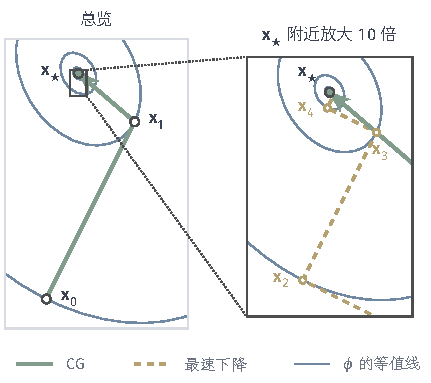
\includegraphics[width=72.873mm]{figures/01-basic-mathematics/03-vectors-matrices-and-multivariate-functions/tikz/c5-cg-steepest-descent-paths/figure.pdf}
  \caption{贯穿例上CG与最速下降的路径。蓝色椭圆是$\phi(\bm x)=\tfrac12\bm x^\top\bm A\bm x-\bm b^\top\bm x$经过最速下降各迭代点的等值线，中心为$\bm x_\star=(1/11,7/11)^\top$。两种方法的第一步都从$\bm x_0=\bm 0$走到$\bm x_1=(1/4,1/2)^\top$；CG的第二个方向与第一个方向$\bm A$共轭，直接指向椭圆中心，最速下降则在$\bm x_\star$附近来回折返（右图为左图小框放大10倍）。}
  \label{fig:ls-cg-steepest-descent-paths}
\end{figure}

\subsection{算法分析}

\paragraph{正确性与收敛速度}
正确性归结为两组关系：残差两两正交，方向两两共轭。由它们可以推出最优性，再由残差多项式得到收敛速度。

\begin{theorem}[CG的最优性与收敛速度]
\label{thm:ls-cg-convergence}
设$\bm A$对称正定，在精确算术下按上述递推计算，且$\bm r_0,\ldots,\bm r_{k-1}$均非零。则$\bm r_0,\ldots,\bm r_k$两两正交，$\bm p_0,\ldots,\bm p_{k-1}$两两关于$\bm A$共轭，$\bm x_k$是$\lVert\bm x-\bm x_\star\rVert_{\bm A}$在$\bm x_0+\mathcal K_k$上的唯一最小点，并且
\begin{equation}
 \lVert\bm x_k-\bm x_\star\rVert_{\bm A}\le2\Bigl(\frac{\sqrt\kappa-1}{\sqrt\kappa+1}\Bigr)^k\lVert\bm x_0-\bm x_\star\rVert_{\bm A},
 \label{eq:ls-cg-convergence-bound}
\end{equation}
其中$\kappa=\kappa_2(\bm A)$。CG至多$d$步得到精确解。
\end{theorem}

\begin{proof}
证明分三步：先证正交与共轭关系，再由它们推出最优性，最后估计收敛速度。

\emph{正交与共轭关系。}对$k$归纳证明：$\bm r_0,\ldots,\bm r_k$两两正交，$\bm p_0,\ldots,\bm p_k$两两共轭，且两组向量都张成$\mathcal K_{k+1}$。$k=0$时显然。设结论对$k$成立，先证$\bm r_{k+1}\perp\mathcal K_{k+1}$。由$\bm p_k=\bm r_k+\beta_{k-1}\bm p_{k-1}$及$\bm r_k\perp\bm p_{k-1}$，
\[
 \bm p_k^\top\bm r_k=\bm r_k^\top\bm r_k ,
\]
于是由步长~\eqref{eq:ls-cg-step}与残差更新~\eqref{eq:ls-cg-update}，
\[
 \bm p_k^\top\bm r_{k+1}=\bm p_k^\top\bm r_k-\alpha_k\bm p_k^\top\bm A\bm p_k=0 .
\]
对$i<k$，由归纳假设中的共轭性，
\[
 \bm p_i^\top\bm r_{k+1}=\bm p_i^\top\bm r_k-\alpha_k\bm p_i^\top\bm A\bm p_k=0 .
\]
$\bm p_0,\ldots,\bm p_k$张成$\mathcal K_{k+1}$，所以$\bm r_{k+1}\perp\mathcal K_{k+1}$，特别地与$\bm r_0,\ldots,\bm r_k$都正交。

再证$\bm p_{k+1}$与此前的方向共轭。对$i<k$，$\bm A\bm p_i\in\mathcal K_{i+2}\subseteq\mathcal K_{k+1}$，故$\bm r_{k+1}^\top\bm A\bm p_i=0$，从而
\[
 \bm p_{k+1}^\top\bm A\bm p_i=\bm r_{k+1}^\top\bm A\bm p_i+\beta_k\bm p_k^\top\bm A\bm p_i=0 .
\]
对$i=k$，由残差更新得$\bm A\bm p_k=(\bm r_k-\bm r_{k+1})/\alpha_k$，再用$\bm r_{k+1}\perp\bm r_k$与式~\eqref{eq:ls-cg-step}、\eqref{eq:ls-cg-beta}，
\[
 \bm r_{k+1}^\top\bm A\bm p_k=-\frac{\bm r_{k+1}^\top\bm r_{k+1}}{\alpha_k}=-\beta_k\,\bm p_k^\top\bm A\bm p_k ,
\]
恰被$\beta_k\bm p_k^\top\bm A\bm p_k$抵消，所以$\bm p_{k+1}^\top\bm A\bm p_k=0$。最后$\bm r_{k+1},\bm p_{k+1}\in\mathcal K_{k+2}$；若$\bm r_{k+1}\ne\bm 0$，两两正交的非零残差线性无关，两组向量都张成$\mathcal K_{k+2}$。

\emph{最优性。}记$\bm e_k=\bm x_k-\bm x_\star$，则$\bm A\bm e_k=-\bm r_k$，且由上一步$\bm r_k\perp\mathcal K_k$。对任意$\bm z\in\mathcal K_k$，
\[
 \lVert\bm e_k+\bm z\rVert_{\bm A}^2
 =\lVert\bm e_k\rVert_{\bm A}^2+2\bm z^\top\bm A\bm e_k+\lVert\bm z\rVert_{\bm A}^2
 =\lVert\bm e_k\rVert_{\bm A}^2+\lVert\bm z\rVert_{\bm A}^2 ,
\]
所以$\bm x_k$是$\bm x_0+\mathcal K_k$上的唯一最小点。$\mathbb R^d$中两两正交的非零向量至多$d$个，故至多$d$步出现零残差。

\emph{收敛速度。}按式~\eqref{eq:ls-krylov-residual-polynomial}的推导，$\bm x_0+\mathcal K_k$中候选的误差为$p(\bm A)\bm e_0$，其中$p\in\mathcal P_k$。由谱定理（定理~\ref{thm:ls-real-symmetric-spectral}）取标准正交特征向量展开$\bm e_0=\sum_ic_i\bm u_i$，得
\[
 \lVert p(\bm A)\bm e_0\rVert_{\bm A}^2=\sum_i\lambda_i\,p(\lambda_i)^2c_i^2\le\max_i p(\lambda_i)^2\,\lVert\bm e_0\rVert_{\bm A}^2 .
\]
由最优性，$\lVert\bm e_k\rVert_{\bm A}$不超过任一$p\in\mathcal P_k$给出的上界，只需构造一个在特征值上很小的$p$。取Chebyshev多项式$T_k$，它由$T_k(\cos\theta)=\cos k\theta$确定，在$[-1,1]$上$\lvert T_k\rvert\le1$；对$x>1$，
\[
 T_k(x)=\tfrac12\bigl[(x+\sqrt{x^2-1})^k+(x-\sqrt{x^2-1})^k\bigr],
\]
因为两边满足同一递推$T_{j+1}=2xT_j-T_{j-1}$和相同初值。令
\[
 \ell(t)=\frac{\lambda_{\max}+\lambda_{\min}-2t}{\lambda_{\max}-\lambda_{\min}},
\]
它把$[\lambda_{\min},\lambda_{\max}]$映到$[-1,1]$，且$\ell(0)=(\kappa+1)/(\kappa-1)$。取
\[
 p(t)=\frac{T_k(\ell(t))}{T_k(\ell(0))}\in\mathcal P_k ,
\]
则在各特征值处$\lvert p\rvert\le1/T_k(\ell(0))$。直接计算，$x=\ell(0)$时$x+\sqrt{x^2-1}=(\sqrt\kappa+1)/(\sqrt\kappa-1)$，于是
\[
 T_k(\ell(0))\ge\frac12\Bigl(\frac{\sqrt\kappa+1}{\sqrt\kappa-1}\Bigr)^k ,
\]
即得所述界。$\kappa=1$时$\bm A$是单位矩阵的倍数，一步得解。
\end{proof}

这个界只依赖两端特征值，误差缩小到给定比例所需的步数约与$\sqrt\kappa$成正比。它控制的是误差的$\bm A$范数，欧氏残差$\lVert\bm r_k\rVert_2$不必每步下降。

\paragraph{数值敏感度}
浮点计算中正交与共轭关系逐步受损，定理的有限步结论不能直接移用，实际计算不承诺恰好$d$步结束；递推残差也会偏离真实残差，所以宣布达到要求前按公共准则用$\bm b-\bm A\bm x_k$复核。

\paragraph{计算代价}
每轮核心递推需要一次$\bm A$乘向量、两次内积和三次向量更新。除矩阵外只保存$\bm x,\bm r,\bm p,\bm q$四个向量，存储不随步数增长；复核真实残差所需的矩阵乘向量另计。

\section{广义最小残差法}
\label{sec:ls-gmres}

设$\bm A$是一般的非奇异方阵，不要求对称或正定。\term{广义最小残差法}（generalized minimal residual method，GMRES）在第$k$步取$\bm x_0+\mathcal K_k$中使原残差长度$\lVert\bm b-\bm A\bm x\rVert_2$最小的近似，与MINRES同样采用第~\ref{sec:ls-krylov-selection-criteria}节的极小残差条件。它紧接第~\ref{sec:ls-arnoldi-application}节：Arnoldi正交化已把这一准则化为一个$(k+1)\times k$的上Hessenberg最小二乘问题，本节说明怎样随步数逐列求解它、怎样读出残差长度并还原近似解。Arnoldi递推本身不再重述，只引用第~\ref{sec:ls-arnoldi}节的式子与定理。

\subsection{主要思想}

\paragraph{逐步长大的小问题}
先看一个周期。记周期的起点为$\bm x^{(s)}$，残差为$\bm r^{(s)}=\bm b-\bm A\bm x^{(s)}$；不重启时只有一个周期，$\bm x^{(s)}=\bm x_0$。令
\begin{equation}
 \beta=\lVert\bm r^{(s)}\rVert_2,\qquad \bm v_1=\frac{\bm r^{(s)}}{\beta},
 \label{eq:ls-gmres-start}
\end{equation}
按式~\eqref{eq:ls-arnoldi-coefficients}与\eqref{eq:ls-arnoldi-normalize}作$j$轮Arnoldi正交化。由定理~\ref{thm:ls-arnoldi-relation}，$\bm V_{j+1}$的列标准正交，并有关系~\eqref{eq:ls-arnoldi-relation}：
\[
 \bm A\bm V_j=\bm V_{j+1}\overline{\bm H}_j .
\]
按第~\ref{sec:ls-arnoldi-application}节，候选写成$\bm x=\bm x^{(s)}+\bm V_j\bm y$，残差等于$\bm V_{j+1}(\beta\bm e_1-\overline{\bm H}_j\bm y)$，而$\bm V_{j+1}$不改变长度，所以
\begin{equation}
 \lVert\bm b-\bm A\bm x\rVert_2=\lVert\beta\bm e_1-\overline{\bm H}_j\bm y\rVert_2 .
 \label{eq:ls-gmres-small-problem}
\end{equation}
GMRES在每一步都要求出使右端最小的$\bm y$。

这个小问题随步数长大。第$j$步的$(j+1)\times j$上Hessenberg矩阵是
\[
 \overline{\bm H}_j=
 \begin{bmatrix}
 h_{1,1}&h_{1,2}&\cdots&h_{1,j-1}&h_{1,j}\\
 h_{2,1}&h_{2,2}&\cdots&h_{2,j-1}&h_{2,j}\\
 &h_{3,2}&\cdots&h_{3,j-1}&h_{3,j}\\
 &&\ddots&\vdots&\vdots\\
 &&&h_{j,j-1}&h_{j,j}\\
 &&&&h_{j+1,j}
 \end{bmatrix}.
\]
与MINRES一样，从第$j-1$步到第$j$步，矩阵只在右侧添了一列、在下方添了一行，已有元素不变。不同的是，新的一列$(h_{1,j},\ldots,h_{j+1,j})^\top$来自Arnoldi正交化中$\bm A\bm v_j$对全部旧基向量的系数，一般全都不为零；新的一行仍只有末元素$h_{j+1,j}$。所以前一步的消元结果仍可沿用，但处理新列的工作比MINRES多。

\paragraph{沿用前一步的消元结果}
小问题用第~\ref{sec:ls-qr-method}节的Givens旋转化为上三角。第$i$个旋转$\bm G_i$只作用于第$i$、$i+1$两行，在这两行上的形式为
\[
 \begin{bmatrix}c_i&s_i\\-s_i&c_i\end{bmatrix},\qquad c_i^2+s_i^2=1 ,
\]
用来消去第$i$列的次对角元。设前$j-1$步已经用$\bm G_1,\ldots,\bm G_{j-1}$把$\overline{\bm H}_{j-1}$消成了上三角，记所得上三角矩阵的元素为$r_{i,l}$。由于$\overline{\bm H}_{j-1}$的各列一般都是满的，这个上三角矩阵也是满的。以$j=4$为例，前三列经过$\bm G_1,\bm G_2,\bm G_3$后成为
\[
 \begin{bmatrix}
 r_{1,1}&r_{1,2}&r_{1,3}\\
 0&r_{2,2}&r_{2,3}\\
 0&0&r_{3,3}\\
 0&0&0
 \end{bmatrix}.
\]
以后的旋转只作用于第$4$行及以下，这三列不再改变。

\paragraph{新列要经过全部旧旋转}
前$j-1$列已经过$\bm G_1,\ldots,\bm G_{j-1}$，新列必须也依次经过这些旧旋转，整个矩阵才是同一个正交变换的结果。新列在第$1$至$j+1$行都可能非零，所以每个旧旋转都会改变它，不能像MINRES那样只用最近两个。旧旋转作用完后，新列在对角线以下只剩第$j+1$行的$h_{j+1,j}$，再构造一个新旋转$\bm G_j$把它消去。

以$j=4$为例，新列逐次旋转的变化为
\[
 \begin{bmatrix}h_{1,4}\\h_{2,4}\\h_{3,4}\\h_{4,4}\\h_{5,4}\end{bmatrix}
 \xrightarrow{\ \bm G_1\ }
 \begin{bmatrix}r_{1,4}\\\ast\\h_{3,4}\\h_{4,4}\\h_{5,4}\end{bmatrix}
 \xrightarrow{\ \bm G_2\ }
 \begin{bmatrix}r_{1,4}\\r_{2,4}\\\ast\\h_{4,4}\\h_{5,4}\end{bmatrix}
 \xrightarrow{\ \bm G_3\ }
 \begin{bmatrix}r_{1,4}\\r_{2,4}\\r_{3,4}\\a\\h_{5,4}\end{bmatrix}
 \xrightarrow{\ \bm G_4\ }
 \begin{bmatrix}r_{1,4}\\r_{2,4}\\r_{3,4}\\\rho_4\\0\end{bmatrix},
\]
其中$\ast$表示被旋转改动、随即又被下一个旋转改动的中间值，$a$是第$4$行在旧旋转作用完后的元素。每个旧旋转$\bm G_i$把第$i$、$i+1$两个分量换成
\[
 \begin{bmatrix}c_i&s_i\\-s_i&c_i\end{bmatrix}
 \begin{bmatrix}h_{i,j}\\h_{i+1,j}\end{bmatrix},
\]
第$i$个分量就此定下，成为$r_{i,j}$。整个矩阵在新旋转之前与之后分别是
\[
 \begin{bmatrix}
 r_{1,1}&r_{1,2}&r_{1,3}&r_{1,4}\\
 0&r_{2,2}&r_{2,3}&r_{2,4}\\
 0&0&r_{3,3}&r_{3,4}\\
 0&0&0&a\\
 0&0&0&h_{5,4}
 \end{bmatrix}
 \xrightarrow{\ \bm G_4\ }
 \begin{bmatrix}
 r_{1,1}&r_{1,2}&r_{1,3}&r_{1,4}\\
 0&r_{2,2}&r_{2,3}&r_{2,4}\\
 0&0&r_{3,3}&r_{3,4}\\
 0&0&0&\rho_4\\
 0&0&0&0
 \end{bmatrix}.
\]
新旋转只处理右下角的$a$与$h_{5,4}$。一般地，记$h=h_{j+1,j}$，新旋转取
\begin{equation}
 \rho_j=\sqrt{a^2+h^2},\qquad c_j=\frac a{\rho_j},\qquad s_j=\frac h{\rho_j},
 \label{eq:ls-gmres-givens}
\end{equation}
把$(a,h)$变为$(\rho_j,0)$，$\rho_j=r_{j,j}$；实际用不会溢出的$\operatorname{hypot}(a,h)$计算$\rho_j$。旋转都要保存下来，供以后各列使用。

\paragraph{右端与残差}
同一组旋转也作用于右端$\beta\bm e_1$。它的第$j+1$个分量起初为零，只有第$j$个旋转才把非零值带下来；记右端为$\bm g$，初值$\bm g=\beta\bm e_1$，则
\begin{equation}
 g_j\leftarrow c_jg_j,\qquad g_{j+1}=-s_jg_j ,
 \label{eq:ls-gmres-rhs}
\end{equation}
右边都用旋转前的$g_j$，前面已确定的分量不变。以$j=4$为例，右端在$\bm G_4$前后分别是
\[
 \begin{bmatrix}g_1\\g_2\\g_3\\g_4\\0\end{bmatrix}
 \xrightarrow{\ \bm G_4\ }
 \begin{bmatrix}g_1\\g_2\\g_3\\c_4g_4\\-s_4g_4\end{bmatrix}.
\]
全部$j$个旋转作用后，小矩阵成为上三角块$\bm R_j$下接一行零。旋转保长，小问题的目标化为
\begin{equation}
 \lVert\beta\bm e_1-\overline{\bm H}_j\bm y\rVert_2^2
 =\lVert(g_1,\ldots,g_j)^\top-\bm R_j\bm y\rVert_2^2+g_{j+1}^2 .
 \label{eq:ls-gmres-rotated-objective}
\end{equation}
前$j$个方程可由上三角的$\bm R_j$精确满足，最后一个分量$g_{j+1}$无论$\bm y$取什么都无法消去，所以最小残差长度就是$\lvert g_{j+1}\rvert$。由式~\eqref{eq:ls-gmres-rhs}，它满足
\[
 \lvert g_{j+1}\rvert=\lvert s_j\rvert\,\lvert g_j\rvert\le\lvert g_j\rvert ,
\]
因而随步数不增。不形成$\bm y$和$\bm x$，每步就能读出残差长度，用来决定何时停下。

\paragraph{与MINRES的差别}
消元的框架与MINRES相同，残差长度也同样随消元得到；差别都来自新列是满的。

其一，每步的工作量随步数增长：第$j$步要作用$j-1$个旧旋转，Arnoldi正交化还要与$j$个旧基向量求内积并扣除，全部旋转与基向量都须保存。

其二，没有短递推。MINRES的$\bm R_k$只有三条非零对角线，可以把$\bm V_k\bm R_k^{-1}$的列写成方向的三项递推，边迭代边累加解；这里$\bm R_j$是满的上三角矩阵，新方向要与全部旧方向组合，而且每增加一列，回代所得$\bm y$的各个分量一般都会改变。所以GMRES不逐步更新$\bm x$，只在停下时由回代
\begin{equation}
 \bm R_j\bm y=(g_1,\ldots,g_j)^\top
 \label{eq:ls-gmres-back-substitution}
\end{equation}
求出系数，再由
\begin{equation}
 \bm x=\bm x^{(s)}+\bm V_j\bm y
 \label{eq:ls-gmres-solution}
\end{equation}
用整组基还原原变量。这组基本来也要用于Arnoldi的扣除，保存它并不额外增加存储。

$\bm A$对称时，由第~\ref{sec:ls-lanczos}节，$\overline{\bm H}_j$成为三对角矩阵，新列只有三个非零元，只需经过两个旧旋转，回代也化为短递推，这就是第~\ref{sec:ls-minres}节的MINRES。

\paragraph{重启}
基的存储与正交化工作都随步数增长，实际常用重启：每个周期最多走$m$步，按式~\eqref{eq:ls-gmres-solution}更新$\bm x$，用原矩阵重算残差，再以它为新周期的$\bm r^{(s)}$重新生成基。重启限制了存储，代价是新周期不再利用旧周期的子空间。

\subsection{算法实现}

输入为非奇异方阵$\bm A$与右端$\bm b$，算法只需计算$\bm A$乘向量，输出为近似解$\bm x$。预先选定初值$\bm x_0$、容差$\mathrm{atol},\mathrm{rtol}$、总步数上限$K$与重启长度$m$（$1\le m\le d$）；停止阈值$\tau$与执行流程沿用第~\ref{sec:ls-matrix-splitting}节，各种结束原因的含义见第~\ref{sec:ls-stationary-stopping}节。

按上一小节的推导，每轮作一轮Arnoldi扩展，让新列经过全部旧旋转，再构造一个新旋转并更新右端，由$\lvert g_{j+1}\rvert$判断是否停下；停下后回代、还原，并从真实残差决定是否重启。下面写出计算中用到的变量、它们怎样初始化、每轮怎样更新。每一步使用例~\ref{ex:ls-stationary-running-example}的数据进行演示，取$m=2$：
\[
 \bm A=\begin{bmatrix}4&1\\1&3\end{bmatrix},\qquad
 \bm b=\begin{bmatrix}1\\2\end{bmatrix},\qquad
 \bm x_0=\bm 0 .
\]
Arnoldi部分的数值与第~\ref{sec:ls-arnoldi}节相同。

\paragraph{变量}
\begin{itemize}
 \item $\bm x^{(s)}\in\mathbb R^d$：本周期的起点，周期结束时更新为新的近似解。
 \item $\bm v_1,\ldots,\bm v_{j+1}\in\mathbb R^d$：本周期的标准正交基，全部保存，回代后用来还原解。
 \item $\bm w\in\mathbb R^d$：Arnoldi的工作向量。
 \item $h_{1,j},\ldots,h_{j+1,j}$：$\overline{\bm H}_j$的第$j$列；经旋转后在原处变为$\bm R_j$的第$j$列，对角元为$\rho_j$，次对角元变为零。
 \item $c_i,s_i$（$i\le j$）：已构造的旋转，全部保存。
 \item $\bm g\in\mathbb R^{j+1}$：经旋转的右端，前$j$个分量用于回代，$\lvert g_{j+1}\rvert$是残差长度的估计。
 \item $j$：本周期内的轮次；另记累计步数，与上限$K$比较。
\end{itemize}

\paragraph{初始化}
把周期起点初始化为$\bm x_0$，计算残差并作停止检查：$\lVert\bm r^{(s)}\rVert_2\le\tau$时以“达到容差”结束，累计步数已达$K$时以“步数耗尽”结束，都输出$\bm x^{(s)}$，不再归一化。否则把第一个基向量初始化为残差的方向，右端初始化为$\beta\bm e_1$，轮次初始化为$1$：
\[
 \begin{gathered}
 \bm x^{(s)}=\bm x_0,\qquad \bm r^{(s)}=\bm b-\bm A\bm x^{(s)},\qquad \beta=\lVert\bm r^{(s)}\rVert_2,\\
 \bm v_1=\frac{\bm r^{(s)}}{\beta},\qquad \bm g=\beta\bm e_1,\qquad j=1 .
 \end{gathered}
\]
重启时以新的$\bm x^{(s)}$回到这里，所以这里的停止检查用的总是原矩阵重算的真实残差。例中$\bm r^{(s)}=\bm b$，
\[
 \beta=\sqrt5,\qquad \bm v_1=\frac1{\sqrt5}\begin{bmatrix}1\\2\end{bmatrix},\qquad \bm g=\begin{bmatrix}\sqrt5\\0\end{bmatrix}.
\]

\paragraph{每轮更新}
在第$j$轮：
\begin{enumerate}
 \item \textbf{Arnoldi扩展。}按第~\ref{sec:ls-arnoldi}节计算过程中每轮更新的第1—3步，即式~\eqref{eq:ls-arnoldi-coefficients}与\eqref{eq:ls-arnoldi-normalize}，计算
 \[
  \begin{gathered}
  \bm w=\bm A\bm v_j ,\\
  h_{i,j}=\bm v_i^\top\bm w,\qquad \bm w\leftarrow\bm w-h_{i,j}\bm v_i\qquad(i=1,\ldots,j),\\
  h_{j+1,j}=\lVert\bm w\rVert_2,\qquad \bm v_{j+1}=\frac{\bm w}{h_{j+1,j}} ,
  \end{gathered}
 \]
 得到$\overline{\bm H}_j$的新列；$h_{j+1,j}=0$时不作归一化，不生成$\bm v_{j+1}$。必要时按该节的办法再正交化。例中第一轮
 \[
  \bm A\bm v_1=\frac1{\sqrt5}\begin{bmatrix}6\\7\end{bmatrix},\qquad
  \begin{bmatrix}h_{1,1}\\h_{2,1}\end{bmatrix}=\begin{bmatrix}4\\1\end{bmatrix},\qquad
  \bm v_2=\frac1{\sqrt5}\begin{bmatrix}2\\-1\end{bmatrix}.
 \]

 \item \textbf{作用旧旋转。}对$i=1,\ldots,j-1$依次计算
 \begin{equation}
  \begin{bmatrix}h_{i,j}\\h_{i+1,j}\end{bmatrix}\leftarrow
  \begin{bmatrix}c_i&s_i\\-s_i&c_i\end{bmatrix}\begin{bmatrix}h_{i,j}\\h_{i+1,j}\end{bmatrix},
  \label{eq:ls-gmres-old-rotations}
 \end{equation}
 每次只改动相邻的两个元素。例中第一轮没有旧旋转，新列仍为$(4,1)^\top$。

 \item \textbf{构造新旋转。}取$a=h_{j,j}$、$h=h_{j+1,j}$，按式~\eqref{eq:ls-gmres-givens}算出$\rho_j,c_j,s_j$并保存，令$h_{j,j}\leftarrow\rho_j$、$h_{j+1,j}\leftarrow0$。$h_{j+1,j}=0$时$s_j=0$，照常完成本列；若$a=h=0$，则$\rho_j=0$，小问题秩亏，要先检查$\bm A$是否奇异、小问题是否相容，不能直接相除。例中第一轮$a=4$、$h=1$，
 \[
  \rho_1=\sqrt{17},\qquad c_1=\frac4{\sqrt{17}},\qquad s_1=\frac1{\sqrt{17}} .
 \]

 \item \textbf{更新右端。}按式~\eqref{eq:ls-gmres-rhs}计算
 \[
  g_{j+1}=-s_jg_j,\qquad g_j\leftarrow c_jg_j ,
 \]
 $\lvert g_{j+1}\rvert$即本轮的残差估计。例中第一轮
 \[
  \bm g=\frac{\sqrt5}{\sqrt{17}}\begin{bmatrix}4\\-1\end{bmatrix},\qquad \lvert g_2\rvert=\sqrt{\frac5{17}}\approx0.542 .
 \]

 \item \textbf{停止。}若$\lvert g_{j+1}\rvert\le\tau$，或第1步给出$h_{j+1,j}=0$（这时$g_{j+1}=0$），或本周期已走$m$轮，或累计步数达到$K$，退出每轮更新，转入回代；否则令$j\leftarrow j+1$，进入下一轮。$\lvert g_{j+1}\rvert$只是小问题上的估计，是否真正结束要在回代、还原之后由初始化中的真实残差检查决定，见第~\ref{sec:ls-stationary-stopping}节。

 例中第一轮$0.542$未达标，$j=1<m$，进入第二轮。若在此退出，回代得
 \[
  y_1=\frac{g_1}{\rho_1}=\frac{4\sqrt5}{17},\qquad
  \bm x_1=y_1\bm v_1=\begin{bmatrix}4/17\\8/17\end{bmatrix},
 \]
 与MINRES的第一步相同。

 第二轮由第1步，$\bm A\bm v_2=(7,-1)^\top/\sqrt5$，
 \[
  h_{1,2}=1,\qquad h_{2,2}=3,\qquad h_{3,2}=0 ;
 \]
 由第2步，前两个元素经$\bm G_1$变为
 \[
  \begin{bmatrix}c_1&s_1\\-s_1&c_1\end{bmatrix}\begin{bmatrix}1\\3\end{bmatrix}
  =\frac1{\sqrt{17}}\begin{bmatrix}7\\11\end{bmatrix};
 \]
 由第3、4步，$a=11/\sqrt{17}$、$h=0$，
 \[
  \rho_2=\frac{11}{\sqrt{17}},\qquad c_2=1,\qquad s_2=0,\qquad g_3=0 ,
 \]
 $g_2$不变。第二轮$h_{3,2}=0$，二维空间已经用尽，退出每轮更新。
\end{enumerate}

\paragraph{回代与重启}
退出后，旋转过的各列组成上三角矩阵$\bm R_j$，按式~\eqref{eq:ls-gmres-back-substitution}自下而上回代求$\bm y$，再按式~\eqref{eq:ls-gmres-solution}还原$\bm x$。然后令$\bm x^{(s)}\leftarrow\bm x$，回到初始化：在那里用原矩阵重算残差并复核，满足阈值或已达累计步数上限就输出，否则从这个残差开始新的周期。若几个周期后真实残差几乎不再下降，应报告停滞，而不是继续无限重启。

例中两轮的结果组成
\[
 \bm R_2=\frac1{\sqrt{17}}\begin{bmatrix}17&7\\0&11\end{bmatrix},\qquad
 (g_1,g_2)^\top=\frac{\sqrt5}{\sqrt{17}}\begin{bmatrix}4\\-1\end{bmatrix},
\]
回代得
\[
 y_2=-\frac{\sqrt5}{11},\qquad y_1=\frac{4\sqrt5-7y_2}{17}=\frac{3\sqrt5}{11},
\]
于是
\[
 \bm x=\bm V_2\bm y=\frac3{11}\begin{bmatrix}1\\2\end{bmatrix}-\frac1{11}\begin{bmatrix}2\\-1\end{bmatrix}=\begin{bmatrix}\tfrac1{11}\\\tfrac7{11}\end{bmatrix}.
\]

最终得到本周期子空间中残差最小的近似解。例中回到初始化后真实残差为零，以“达到容差”结束，输出
\[
 \bm x_\star=\begin{bmatrix}\tfrac1{11}\\\tfrac7{11}\end{bmatrix} .
\]
代回核对：
\[
 \bm A\bm x_\star=\begin{bmatrix}4/11+7/11\\1/11+21/11\end{bmatrix}=\begin{bmatrix}1\\2\end{bmatrix}=\bm b ,
\]
与MINRES的结果相同；$\bm R_2$与$\bm g$也正是把第~\ref{sec:ls-arnoldi}节的$\overline{\bm H}_2$与$\sqrt5\,\bm e_1$用同两个旋转变换的结果。

贯穿例的矩阵是对称的，小矩阵也对称。下面换用非对称矩阵，这是MINRES不再适用、GMRES仍然可用的情形。

\begin{example}[非对称矩阵上的GMRES]
\label{ex:ls-gmres-nonsymmetric}
下面用以下数据演示，取$m=2$：
\[
 \bm A=\begin{bmatrix}3&1\\0&2\end{bmatrix},\qquad
 \bm b=\begin{bmatrix}1\\1\end{bmatrix},\qquad
 \bm x_0=\bm0 .
\]
于是$\bm r_0=\bm b$，$\beta=\sqrt2$，$\bm v_1=(1,1)^\top/\sqrt2$。

第一轮由第1步，$\bm A\bm v_1=(4,2)^\top/\sqrt2$，得新列与新基向量
\[
 \begin{bmatrix}h_{1,1}\\h_{2,1}\end{bmatrix}=\begin{bmatrix}3\\1\end{bmatrix},\qquad
 \bm v_2=\frac1{\sqrt2}\begin{bmatrix}1\\-1\end{bmatrix}.
\]
由第3、4步，
\[
 \rho_1=\sqrt{10},\qquad c_1=\frac3{\sqrt{10}},\qquad s_1=\frac1{\sqrt{10}},\qquad
 \bm g=\frac1{\sqrt5}\begin{bmatrix}3\\-1\end{bmatrix}.
\]
若在此结束，回代得
\[
 y_1=\frac{3\sqrt2}{10},\qquad \bm x_1=y_1\bm v_1=\begin{bmatrix}3/10\\3/10\end{bmatrix}.
\]
直接计算原残差
\[
 \bm r_1=\bm b-\bm A\bm x_1=\begin{bmatrix}-1/5\\2/5\end{bmatrix},\qquad
 \lVert\bm r_1\rVert_2=\frac1{\sqrt5}=\lvert g_2\rvert .
\]

第二轮$\bm A\bm v_2=2\bm v_2$，新列为$(0,2,0)^\top$，与对角线下方的$h_{2,1}=1$不对称。由第2步，它经$\bm G_1$变为
\[
 \begin{bmatrix}2/\sqrt{10}\\6/\sqrt{10}\\0\end{bmatrix};
\]
由于$h_{3,2}=0$，新旋转为$c_2=1$、$s_2=0$，$g_3=0$。回代
\[
 \begin{bmatrix}\sqrt{10}&2/\sqrt{10}\\0&6/\sqrt{10}\end{bmatrix}\begin{bmatrix}y_1\\y_2\end{bmatrix}=\frac1{\sqrt5}\begin{bmatrix}3\\-1\end{bmatrix}
\]
得$y_2=-\sqrt2/6$、$y_1=\sqrt2/3$，恢复出
\[
 \bm x_2=\frac13\begin{bmatrix}1\\1\end{bmatrix}-\frac16\begin{bmatrix}1\\-1\end{bmatrix}=\begin{bmatrix}\tfrac16\\\tfrac12\end{bmatrix},
\]
代回得$\bm A\bm x_2=(1/2+1/2,\,1)^\top=\bm b$，原残差为零。两轮中的Arnoldi系数可以按第~\ref{sec:ls-arnoldi}节的计算过程逐步核对。
\end{example}

\subsection{算法分析}

\paragraph{正确性}
下面的定理针对不重启的完整GMRES，即$m=d$、$\bm x^{(s)}=\bm x_0$的情形。

\begin{theorem}[GMRES的最小残差性]
\label{thm:ls-gmres-optimality}
设$\bm A$非奇异，在精确算术下执行完整GMRES的第$k$步，记$\bm r_k=\bm b-\bm A\bm x_k$。则$\bm x_k$是$\bm x_0+\mathcal K_k$中残差长度的唯一最小点，$\lVert\bm r_k\rVert_2=\lvert g_{k+1}\rvert$，它等于上一步的残差长度乘以$\lvert s_k\rvert\le1$，因而随$k$不增；GMRES至多$d$步得到精确解。若$\bm A=\bm X\bm\Lambda\bm X^{-1}$可对角化（$\bm X,\bm\Lambda$可以是复矩阵），还有
\begin{equation}
 \lVert\bm r_k\rVert_2\le\kappa_2(\bm X)\min_{p\in\mathcal P_k}\max_{\lambda\in\sigma(\bm A)}\lvert p(\lambda)\rvert\,\lVert\bm r_0\rVert_2,
 \label{eq:ls-gmres-residual-bound}
\end{equation}
其中$\mathcal P_k$同引理~\ref{lem:ls-krylov-residual-polynomial}。
\end{theorem}

\begin{proof}
证明分四步：先把原问题化为小问题，再由旋转求出小问题的解与最小值，然后说明单调性与有限步终止，最后由残差多项式得到界。

\emph{化为小问题。}由Arnoldi关系（定理~\ref{thm:ls-arnoldi-relation}），Arnoldi尚未停止时$\bm V_{k+1}$的列标准正交，且$\bm A\bm V_k=\bm V_{k+1}\overline{\bm H}_k$。由$\bm r_0=\beta\bm V_{k+1}\bm e_1$，
\[
 \bm b-\bm A(\bm x_0+\bm V_k\bm y)=\bm r_0-\bm A\bm V_k\bm y=\bm V_{k+1}(\beta\bm e_1-\overline{\bm H}_k\bm y),
\]
乘以$\bm V_{k+1}$不改变长度，即得式~\eqref{eq:ls-gmres-small-problem}。$\bm V_k$满列秩，$\bm y\mapsto\bm x_0+\bm V_k\bm y$是$\mathbb R^k$到$\bm x_0+\mathcal K_k$的双射，两个最小化问题的解一一对应。

\emph{旋转后的小问题。}记$k$个旋转之积为正交矩阵$\bm\Omega_k$。每个新旋转只作用于第$j,j+1$行，而新列在此前已经过全部旧旋转，所以
\[
 \bm\Omega_k\overline{\bm H}_k=\begin{bmatrix}\bm R_k\\\bm 0^\top\end{bmatrix},\qquad
 \bm\Omega_k\beta\bm e_1=\bm g=(g_1,\ldots,g_{k+1})^\top ,
\]
从而
\[
 \lVert\beta\bm e_1-\overline{\bm H}_k\bm y\rVert_2^2
 =\lVert(g_1,\ldots,g_k)^\top-\bm R_k\bm y\rVert_2^2+g_{k+1}^2 .
\]
$\bm A$非奇异且$\bm V_k$满列秩，$\bm A\bm V_k=\bm V_{k+1}\overline{\bm H}_k$满列秩，故$\overline{\bm H}_k$与$\bm R_k$满秩，$\bm R_k$可逆。回代~\eqref{eq:ls-gmres-back-substitution}所得的$\bm y$使第一项为零，且是唯一使之为零的点，最小值为$\lvert g_{k+1}\rvert$。

\emph{单调性与有限步终止。}第$k$个旋转把旋转前的$g_k$变为$c_kg_k$与$-s_kg_k$，而旋转前的$\lvert g_k\rvert$正是上一步的残差长度，所以
\[
 \lvert g_{k+1}\rvert=\lvert s_k\rvert\,\lvert g_k\rvert\le\lvert g_k\rvert .
\]
若$h_{k+1,k}=0$，则$s_k=0$，$g_{k+1}=0$，残差为零；子空间维数不超过$d$，所以至多$d$步出现这一情形或零残差。

\emph{残差界。}由引理~\ref{lem:ls-krylov-residual-polynomial}与最小残差性，
\[
 \lVert\bm r_k\rVert_2=\min_{p\in\mathcal P_k}\lVert p(\bm A)\bm r_0\rVert_2 .
\]
而$p(\bm A)=\bm X\,p(\bm\Lambda)\bm X^{-1}$，对角矩阵$p(\bm\Lambda)$的谱范数是$\max_{\lambda\in\sigma(\bm A)}\lvert p(\lambda)\rvert$，于是
\[
 \lVert p(\bm A)\bm r_0\rVert_2\le\lVert\bm X\rVert_2\lVert\bm X^{-1}\rVert_2\max_{\lambda\in\sigma(\bm A)}\lvert p(\lambda)\rvert\,\lVert\bm r_0\rVert_2 ,
\]
其中$\lVert\bm X\rVert_2\lVert\bm X^{-1}\rVert_2=\kappa_2(\bm X)$，对$p$取最小即得所述界。
\end{proof}

\paragraph{收敛速度}
定理中的界把收敛问题化为多项式逼近：要找在原点取值$1$、在全部特征值上都很小的低次多项式。非正规矩阵的$\kappa_2(\bm X)$可能很大，界因此变弱，只看特征值是否集中不能判断收敛快慢。

\paragraph{重启与数值敏感度}
重启的GMRES($m$)丢弃了历史空间：每个周期内的残差仍最小，但这只是在本周期子空间上的最优，不能说成累计全部历史空间上的最优。它可能停滞，也不再有$d$步得到精确解的保证。浮点计算中基不再精确正交，$\lvert g_{j+1}\rvert$与真实残差会偏离，这就是每个周期结束时用$\bm b-\bm A\bm x$复核的原因。

\paragraph{计算代价}
每轮需要一次$\bm A$乘向量。完整GMRES执行$k$步时，正交化共约$2dk^2$次浮点运算，基的存储约$kd$个数，都随步数增长；GMRES($m$)把历史基限制在一个周期内，每周期至多约$2dm^2$次运算，存储约$(m+1)d$个数，与总步数无关。

\section{双共轭梯度法}
\label{sec:ls-bicg}

第~\ref{sec:ls-arnoldi-application}节说明，对一般方阵，Arnoldi正交化给出的小问题无论按Galerkin条件还是按极小残差条件求解，都要用整组基还原近似解；GMRES（第~\ref{sec:ls-gmres}节）因此须保存全部基向量，存储与正交化工作随步数线性增长。

第~\ref{sec:ls-lanczos-application}节的短递推则依赖对称性：正是$\bm A^\top=\bm A$使大部分系数$h_{i,j}$为零，MINRES与CG才只需固定数量的向量。

本节的双共轭梯度法针对一般的非对称可逆方阵，改用第~\ref{sec:ls-krylov-selection-criteria}节第四类准则中的影子空间：残差不再与$\mathcal K_k$本身正交，而与$\bm A^\top$生成的Krylov子空间正交，即Petrov--Galerkin条件~\eqref{eq:ls-krylov-projection}。这样恢复了短递推，算法形式与CG的式~\eqref{eq:ls-cg-update}—\eqref{eq:ls-cg-beta}相仿，代价是放弃残差的最小化；下一节的BiCGSTAB在此基础上减缓残差的起伏。

\subsection{主要思想}

设$\bm A$是一般的实可逆方阵，不要求对称。

\paragraph{影子空间}
对一般的非对称矩阵，在单一的Krylov子空间$\mathcal K_k(\bm A,\bm r_0)$中，短递推与最优性一般不能兼得：GMRES保住了残差最小，却要保存整组基；Lanczos过程的短递推则依赖$\bm A^\top=\bm A$。

BiCG的做法是放弃最优性、保住短递推。为此，除了原方程$\bm A\bm x=\bm b$，它还引入一个以$\bm A^\top$为系数的影子方程，从满足$\widetilde{\bm r}_0^\top\bm r_0\ne0$的影子残差$\widetilde{\bm r}_0$出发，生成影子空间$\mathcal K_k(\bm A^\top,\widetilde{\bm r}_0)$。近似仍取在$\bm x_0+\mathcal K_k(\bm A,\bm r_0)$中，但要求残差与影子空间正交：
\[
 \bm r_k\perp\mathcal K_k(\bm A^\top,\widetilde{\bm r}_0),
\]
即第~\ref{sec:ls-krylov-selection-criteria}节的Petrov--Galerkin条件~\eqref{eq:ls-krylov-projection}。\term{双共轭梯度法}（biconjugate gradient method，BiCG）就按这一条件选取近似。下面看这个条件怎样化成一个三对角方程，以及怎样像CG那样逐步求解它。

\paragraph{双正交的两组基}
设$\bm V_k$的列$\bm v_1,\ldots,\bm v_k$是$\mathcal K_k(\bm A,\bm r_0)$的一组基，$\bm W_k$的列$\bm w_1,\ldots,\bm w_k$是$\mathcal K_k(\bm A^\top,\widetilde{\bm r}_0)$的一组基，且两者的前$j$列分别张成$\mathcal K_j(\bm A,\bm r_0)$与$\mathcal K_j(\bm A^\top,\widetilde{\bm r}_0)$。第~\ref{sec:ls-lanczos}节推导三项递推时，用对称性把$\bm v_i^\top\bm A\bm v_j$改写为$(\bm A\bm v_i)^\top\bm v_j$；没有对称性时，转置把$\bm A$换成$\bm A^\top$，
\[
 \bm w_i^\top\bm A\bm v_j=(\bm A^\top\bm w_i)^\top\bm v_j ,
\]
而$\bm A^\top\bm w_i$正好留在影子空间中。于是要求两组基\term{双正交}（biorthogonality），并归一化为
\begin{equation}
 \bm w_i^\top\bm v_j=\begin{cases}1,&i=j,\\0,&i\ne j,\end{cases}\qquad\text{即}\quad \bm W_k^\top\bm V_k=\bm I .
 \label{eq:ls-bicg-biorthonormal}
\end{equation}
这时$\bm v_j$与$\mathcal K_{j-1}(\bm A^\top,\widetilde{\bm r}_0)$正交，$\bm w_i$与$\mathcal K_{i-1}(\bm A,\bm r_0)$正交。又因为
\[
 \bm A^\top\bm w_i\in\mathcal K_{i+1}(\bm A^\top,\widetilde{\bm r}_0),\qquad \bm A\bm v_j\in\mathcal K_{j+1}(\bm A,\bm r_0),
\]
所以
\[
 \bm w_i^\top\bm A\bm v_j=0\qquad(\lvert i-j\rvert>1),
\]
因此投影矩阵$\bm T_k=\bm W_k^\top\bm A\bm V_k$是三对角的，但一般不对称。

记它的对角元为$a_j$、次对角元为$\gamma_j$、上对角元为$\eta_j$，以$k=3$为例，
\[
 \bm T_3=\begin{bmatrix}a_1&\eta_1&0\\\gamma_1&a_2&\eta_2\\0&\gamma_2&a_3\end{bmatrix}.
\]
与Lanczos过程一样，这两组基可以用三项递推交替生成：
\begin{equation}
 \begin{gathered}
 \bm A\bm v_j=\eta_{j-1}\bm v_{j-1}+a_j\bm v_j+\gamma_j\bm v_{j+1},\\
 \bm A^\top\bm w_j=\gamma_{j-1}\bm w_{j-1}+a_j\bm w_j+\eta_j\bm w_{j+1},
 \end{gathered}
 \label{eq:ls-bicg-two-sided-lanczos}
\end{equation}
每个新基向量只需扣除两个旧方向，称为双边Lanczos过程。若某一步扣除后的两个余项内积为零而余项本身不为零，就无法归一化，递推中断。

\paragraph{逐步长大的三对角方程}
取$\bm v_1=\bm r_0/\beta$，$\beta=\lVert\bm r_0\rVert_2$，并取$\bm w_1$与$\widetilde{\bm r}_0$同向、满足$\bm w_1^\top\bm v_1=1$。把近似写成
\[
  \bm x_k=\bm x_0+\bm V_k\bm y_k ,
\]
Petrov--Galerkin条件是
\[
  \bm W_k^\top(\bm r_0-\bm A\bm V_k\bm y_k)=\bm 0 .
\]
由$\bm W_k^\top\bm V_k=\bm I$得
\[
  \bm W_k^\top\bm r_0=\beta\bm e_1 ,
\]
于是条件化为$k$阶三对角方程
\begin{equation}
 \bm T_k\bm y_k=\beta\bm e_1 .
 \label{eq:ls-bicg-tridiagonal-system}
\end{equation}

这与CG的处境完全相同：每一步$\bm T_k$只在右侧添一列、在下方添一行，新添的元素只有$\eta_{k-1},\gamma_{k-1},a_k$。区别只在于$\bm T_k$不对称，也不一定正定。

\paragraph{分解的增量更新}
不对称的三对角矩阵不能作$\bm L\bm D\bm L^\top$分解，改作不选主元的LU分解：
\[
 \bm T_k=\bm L_k\bm U_k ,
\]
其中$\bm L_k$是单位下双对角矩阵，次对角元记为$\ell_j$；$\bm U_k$是上双对角矩阵，对角元记为$d_j$。

以$k=3$为例，
\[
 \bm L_3\bm U_3=
 \begin{bmatrix}1&&\\\ell_1&1&\\&\ell_2&1\end{bmatrix}
 \begin{bmatrix}d_1&\eta_1&\\&d_2&\eta_2\\&&d_3\end{bmatrix}
 =\begin{bmatrix}d_1&\eta_1&\\\ell_1d_1&\ell_1\eta_1+d_2&\eta_2\\&\ell_2d_2&\ell_2\eta_2+d_3\end{bmatrix}.
\]
$\bm U_k$的上对角元就是$\bm T_k$的$\eta_j$。

与$\bm T_3$逐元素比较，从$d_1=a_1$出发，逐个算出
\begin{equation}
 \ell_j=\frac{\gamma_j}{d_j},\qquad d_{j+1}=a_{j+1}-\ell_j\eta_j\qquad(j=1,2,\ldots).
 \label{eq:ls-bicg-lu}
\end{equation}
对称时$\eta_j=\gamma_j$，这就是CG的式~\eqref{eq:ls-cg-ldl}。与CG一样，$\bm T_{k+1}$只多出$\eta_k,\gamma_k,a_{k+1}$，$\bm L_k,\bm U_k$原封不动，只需在末尾追加$\ell_k$与$d_{k+1}$。不同的是，这里没有正定性保证$d_j\ne0$；若某个$d_j=0$，不选主元的LU就无法继续，这是BiCG的另一种中断。

\paragraph{翻译回向量}
仍按CG的办法把分解翻译成向量的短递推。先由前代$\bm L_k\bm g=\beta\bm e_1$得
\[
 g_1=\beta,\qquad g_{j+1}=-\ell_jg_j ,
\]
再令$\widehat{\bm P}_k=\bm V_k\bm U_k^{-1}=[\hat{\bm p}_1,\ldots,\hat{\bm p}_k]$，则
\[
 \bm x_k=\bm x_0+\widehat{\bm P}_k\bm g .
\]

比较$\widehat{\bm P}_k\bm U_k=\bm V_k$的第$j+1$列，得
\[
 \eta_j\hat{\bm p}_j+d_{j+1}\hat{\bm p}_{j+1}=\bm v_{j+1} .
\]

由于$\bm g$与$\widehat{\bm P}_k$都只在末尾追加，解可以逐步累加：
\[
 \bm x_k=\bm x_{k-1}+g_k\hat{\bm p}_k ,
\]
其中的方向由上式逐列解出：
\[
 \hat{\bm p}_1=\frac{\bm v_1}{d_1},\qquad \hat{\bm p}_{j+1}=\frac{\bm v_{j+1}-\eta_j\hat{\bm p}_j}{d_{j+1}} .
\]
残差也与CG一样落在下一个基向量的方向上。

由$\bm A\bm V_k=\bm V_k\bm T_k+\gamma_k\bm v_{k+1}\bm e_k^\top$与$\bm T_k\bm y_k=\beta\bm e_1$，
\[
 \bm r_k=-\gamma_k(\bm e_k^\top\bm y_k)\bm v_{k+1} .
\]

$\bm U_k\bm y_k=\bm g$的最后一个方程给出$d_k(\bm e_k^\top\bm y_k)=g_k$，所以
\begin{equation}
 \bm r_k=-\ell_kg_k\,\bm v_{k+1}=g_{k+1}\bm v_{k+1} .
 \label{eq:ls-bicg-residual-direction}
\end{equation}
影子方程一侧对$\bm T_k^\top=\bm U_k^\top\bm L_k^\top$作同样的推导，影子残差$\widetilde{\bm r}_k$落在$\bm w_{k+1}$的方向上。于是BiCG可以像CG那样，用残差代替基向量，不必显式生成两组基。

\paragraph{BiCG的形式}
把方向按残差的比例缩放，记
\[
 \bm p_k=g_{k+1}d_{k+1}\hat{\bm p}_{k+1} .
\]

上面的方向递推乘以$g_{k+1}d_{k+1}$，并用$g_{k+1}/g_k=-\ell_k$，就成为
\[
 \bm p_k=\bm r_k+(\ell_k\eta_k/d_k)\bm p_{k-1} .
\]

解的递推成为
\[
 \bm x_{k+1}=\bm x_k+\bm p_k/d_{k+1} .
\]

影子一侧得到同样的系数。于是解、原残差与影子残差用同一个步长更新：
\begin{equation}
 \begin{gathered}
 \bm x_{k+1}=\bm x_k+\alpha_k\bm p_k,\\
 \bm r_{k+1}=\bm r_k-\alpha_k\bm A\bm p_k,\qquad
 \widetilde{\bm r}_{k+1}=\widetilde{\bm r}_k-\alpha_k\bm A^\top\widetilde{\bm p}_k ,
 \end{gathered}
 \label{eq:ls-bicg-update}
\end{equation}
两组方向都从各自的初始残差出发，用同一个组合系数更新：
\begin{equation}
 \begin{gathered}
 \bm p_0=\bm r_0,\qquad \widetilde{\bm p}_0=\widetilde{\bm r}_0,\\
 \bm p_{k+1}=\bm r_{k+1}+\beta_k\bm p_k,\qquad
 \widetilde{\bm p}_{k+1}=\widetilde{\bm r}_{k+1}+\beta_k\widetilde{\bm p}_k ,
 \end{gathered}
 \label{eq:ls-bicg-direction}
\end{equation}
两个系数正是LU分解的元素换算而来：
\[
 \alpha_k=\frac1{d_{k+1}},\qquad \beta_k=\frac{\ell_{k+1}\eta_{k+1}}{d_{k+1}}=\frac{\gamma_{k+1}\eta_{k+1}}{d_{k+1}^2} .
\]
对称时$\eta=\gamma$，这就回到CG的$\beta_k=\ell_{k+1}^2$。

实际计算时不必先求$d_j,\ell_j$。记配对量$\rho_k=\widetilde{\bm r}_k^\top\bm r_k$，两个系数可以直接由向量算出：
\begin{equation}
 \alpha_k=\frac{\rho_k}{\widetilde{\bm p}_k^\top\bm A\bm p_k},
 \label{eq:ls-bicg-step}
\end{equation}
\begin{equation}
 \beta_k=\frac{\rho_{k+1}}{\rho_k}.
 \label{eq:ls-bicg-beta}
\end{equation}
它们与CG的式~\eqref{eq:ls-cg-step}、\eqref{eq:ls-cg-beta}同形，只是内积的一侧换成了影子序列：$\alpha_k$使新原残差与当前影子方向正交，
\[
 \widetilde{\bm p}_k^\top\bm r_{k+1}=0 ;
\]
$\beta_k$使新原方向与当前影子方向关于$\bm A$双共轭，
\[
 \widetilde{\bm p}_k^\top\bm A\bm p_{k+1}=0 .
\]

定理~\ref{thm:ls-bicg-biorthogonality}说明，按式~\eqref{eq:ls-bicg-update}—\eqref{eq:ls-bicg-beta}逐步计算，原、影子残差两两双正交，原、影子方向两两双共轭，所得近似正好满足Petrov--Galerkin条件。$\bm A$对称且$\widetilde{\bm r}_0=\bm r_0$时，影子序列与原序列逐项相同，这组递推就退化为CG。

\paragraph{代价}
BiCG用影子空间换来了短递推，代价有三。

其一，Petrov--Galerkin条件不最小化任何范数，残差的历史可能剧烈振荡。

其二，每步除了$\bm A$乘向量，还要计算一次$\bm A^\top$乘向量。

其三，递推可能中断：$\rho_k=0$而$\bm r_k\ne\bm0$对应双边Lanczos过程无法归一化，$\widetilde{\bm p}_k^\top\bm A\bm p_k=0$对应LU分解中$d_{k+1}=0$。这些在算法分析中具体说明；下一节的BiCGSTAB去掉$\bm A^\top$并减缓振荡。

\subsection{算法实现}

输入为实可逆方阵$\bm A$与右端$\bm b$，算法需要计算$\bm A$与$\bm A^\top$乘向量，输出为近似解$\bm x$。预先选定的参数除第~\ref{sec:ls-matrix-splitting}节执行流程中的初值$\bm x_0$、容差$\mathrm{atol},\mathrm{rtol}$与最大轮数$K$外，还有影子初值$\widetilde{\bm r}_0$，默认取$\widetilde{\bm r}_0=\bm r_0$；停止检查沿用该流程的阈值$\tau=\mathrm{atol}+\mathrm{rtol}\lVert\bm b\rVert_2$，各种结束原因的含义见第~\ref{sec:ls-stationary-stopping}节。

每轮作一次$\bm A$乘向量和一次$\bm A^\top$乘向量，用同一个步长更新解与两个残差，再用同一个组合系数形成两个新方向。与CG不同，$\rho_k$与$\widetilde{\bm p}_k^\top\bm A\bm p_k$不受正定性保护，残差非零时也可能为零，所以每次相除前都要检查分母，并区分收敛与中断。

对称矩阵配上$\widetilde{\bm r}_0=\bm r_0$时BiCG与CG的计算完全一致，贯穿例显示不出影子序列的作用；因此改用把贯穿例的$a_{2,1}$由$1$改为$2$的非对称矩阵，在下面的例子上执行。

\begin{example}[非对称二阶系统上的BiCG]
\label{ex:ls-bicg-two-steps}
取
\[
 \bm A=\begin{bmatrix}4&1\\2&3\end{bmatrix},\qquad
 \bm b=\begin{bmatrix}1\\2\end{bmatrix},\qquad
 \bm x_0=\bm 0,
\]
影子初值$\widetilde{\bm r}_0=\bm r_0$。精确解为
\[
 \bm x_\star=\begin{bmatrix}1/10\\3/5\end{bmatrix},
\]
代回两行方程，$4/10+3/5=1$，$2/10+9/5=2$。下面每一步之后给出BiCG在这个例子上的数值。
\end{example}

\paragraph{变量}
\begin{itemize}
 \item $\bm x\in\mathbb R^d$：当前近似解$\bm x_k$。
 \item $\bm r,\widetilde{\bm r}\in\mathbb R^d$：当前残差$\bm r_k$与影子残差$\widetilde{\bm r}_k$。
 \item $\bm p,\widetilde{\bm p}\in\mathbb R^d$：当前方向$\bm p_k$与影子方向$\widetilde{\bm p}_k$。
 \item $\bm q,\widetilde{\bm q}\in\mathbb R^d$：工作向量，分别存$\bm A\bm p_k$与$\bm A^\top\widetilde{\bm p}_k$，供残差更新复用。
 \item $\rho_k$：配对量$\widetilde{\bm r}_k^\top\bm r_k$，留到下一轮作$\beta_k$的分母。
 \item $\alpha_k,\beta_k$：本轮的步长与组合系数。
 \item $k$：轮次。
\end{itemize}
除矩阵外共保存七个向量，存储不随轮数增长。

\paragraph{初始化}
把解初始化为$\bm x_0$，残差初始化为初始残差，影子残差初始化为影子初值，两组方向分别初始化为两个残差，配对量初始化为两者的内积，轮次初始化为$0$：
\[
 \begin{gathered}
 \bm r_0=\bm b-\bm A\bm x_0,\qquad \bm p_0=\bm r_0,\qquad \widetilde{\bm p}_0=\widetilde{\bm r}_0,\\
 \rho_0=\widetilde{\bm r}_0^\top\bm r_0,\qquad k=0 .
 \end{gathered}
\]
若$\lVert\bm r_0\rVert_2\le\tau$，复核后直接输出$\bm x_0$；若$\rho_0=0$，须另取影子初值。例中
\[
 \bm r_0=\widetilde{\bm r}_0=\bm p_0=\widetilde{\bm p}_0=\begin{bmatrix}1\\2\end{bmatrix},\qquad \rho_0=5,
\]
$\lVert\bm r_0\rVert_2=\sqrt5\approx2.24$，开始迭代。

\paragraph{每轮更新}
在第$k$轮：
\begin{enumerate}
 \item \textbf{乘矩阵。}计算
 \[
  \bm q=\bm A\bm p_k,\qquad \widetilde{\bm q}=\bm A^\top\widetilde{\bm p}_k .
 \]
 例中第一轮
 \[
  \bm q=\begin{bmatrix}6\\8\end{bmatrix},\qquad
  \widetilde{\bm q}=\begin{bmatrix}8\\7\end{bmatrix}.
 \]

 \item \textbf{求步长。}计算分母$\widetilde{\bm p}_k^\top\bm q$。它为零而残差非零时递推中断，报告中断并停止；否则按式~\eqref{eq:ls-bicg-step}，
 \[
  \alpha_k=\frac{\rho_k}{\widetilde{\bm p}_k^\top\bm q} .
 \]
 例中第一轮
 \[
  \widetilde{\bm p}_0^\top\bm q=22,\qquad \alpha_0=\frac5{22}.
 \]

 \item \textbf{更新解与两个残差。}按式~\eqref{eq:ls-bicg-update}，其中$\bm A\bm p_k$与$\bm A^\top\widetilde{\bm p}_k$直接取已算出的$\bm q$与$\widetilde{\bm q}$：
 \[
  \bm x_{k+1}=\bm x_k+\alpha_k\bm p_k,\qquad
  \bm r_{k+1}=\bm r_k-\alpha_k\bm q,\qquad
  \widetilde{\bm r}_{k+1}=\widetilde{\bm r}_k-\alpha_k\widetilde{\bm q} .
 \]
 例中第一轮
 \[
  \bm x_1=\begin{bmatrix}\tfrac5{22}\\\tfrac5{11}\end{bmatrix},\qquad
  \bm r_1=\begin{bmatrix}-\tfrac4{11}\\\tfrac2{11}\end{bmatrix},\qquad
  \widetilde{\bm r}_1=\begin{bmatrix}-\tfrac9{11}\\\tfrac9{22}\end{bmatrix}.
 \]
 可以核对双正交关系
 \[
  \widetilde{\bm r}_0^\top\bm r_1=-\tfrac4{11}+\tfrac4{11}=0,\qquad
  \widetilde{\bm r}_1^\top\bm r_0=-\tfrac9{11}+\tfrac9{11}=0 .
 \]

 \item \textbf{形成新方向。}计算新的配对量，按式~\eqref{eq:ls-bicg-beta}算出组合系数，再按式~\eqref{eq:ls-bicg-direction}形成两个新方向：
 \[
  \rho_{k+1}=\widetilde{\bm r}_{k+1}^\top\bm r_{k+1},\qquad \beta_k=\frac{\rho_{k+1}}{\rho_k},
 \]
 \[
  \bm p_{k+1}=\bm r_{k+1}+\beta_k\bm p_k,\qquad
  \widetilde{\bm p}_{k+1}=\widetilde{\bm r}_{k+1}+\beta_k\widetilde{\bm p}_k .
 \]
 分母$\rho_k$已在初始化或上一轮确认非零。例中第一轮
 \[
  \rho_1=\frac{36}{121}+\frac9{121}=\frac{45}{121},\qquad \beta_0=\frac{45/121}{5}=\frac9{121},
 \]
 \[
  \bm p_1=\begin{bmatrix}-\tfrac{35}{121}\\\tfrac{40}{121}\end{bmatrix},\qquad
  \widetilde{\bm p}_1=\begin{bmatrix}-\tfrac{90}{121}\\\tfrac{135}{242}\end{bmatrix}.
 \]
 可以核对双共轭关系
 \[
  \widetilde{\bm p}_0^\top\bm A\bm p_1=\widetilde{\bm q}^\top\bm p_1=\frac{-280+280}{121}=0 .
 \]
 然后令$k\leftarrow k+1$。

 例中第二轮
 \[
  \bm q=\begin{bmatrix}-\tfrac{100}{121}\\\tfrac{50}{121}\end{bmatrix},\qquad
  \widetilde{\bm q}=\begin{bmatrix}-\tfrac{225}{121}\\\tfrac{225}{242}\end{bmatrix},
 \]
 其中$\widetilde{\bm p}_0^\top\bm q=(-100+100)/121=0$再次印证双共轭。分母与步长为
 \[
  \widetilde{\bm p}_1^\top\bm q=\frac{1125}{1331},\qquad
  \alpha_1=\frac{45/121}{1125/1331}=\frac{11}{25},
 \]
 于是
 \[
  \begin{gathered}
  \bm x_2=\bm x_1+\frac{11}{25}\bm p_1=\begin{bmatrix}\tfrac1{10}\\\tfrac35\end{bmatrix},\\
  \bm r_2=\bm r_1-\frac{11}{25}\bm q=\bm 0,\qquad
  \widetilde{\bm r}_2=\widetilde{\bm r}_1-\frac{11}{25}\widetilde{\bm q}=\bm 0,
  \end{gathered}
 \]
 $\rho_2=0$，$\beta_1=0$。

 \item \textbf{停止。}若$\lVert\bm r_{k}\rVert_2\le\tau$，先用原矩阵重算$\bm b-\bm A\bm x_{k}$复核（第~\ref{sec:ls-stationary-stopping}节），复核仍满足时以“达到容差”结束；若$\bm r_{k}\ne\bm 0$而$\rho_{k}=0$，下一轮的组合系数无法再除以它，以“中断”结束，不能把它当作收敛；若$k=K$，以“步数耗尽”结束；残差长期不降时按停滞处理。各种情况都输出$\bm x_{k}$并报告原因，否则进入下一轮。

 例中第一轮后$\lVert\bm r_1\rVert_2=\sqrt{20}/11\approx0.41$且$\rho_1\ne0$，继续；第二轮后$\bm r_2=\bm 0$，复核真实残差也为零，以“达到容差”结束。
\end{enumerate}
第1—4步就是式~\eqref{eq:ls-bicg-update}—\eqref{eq:ls-bicg-beta}，其中两次矩阵作用都只算一次，存入$\bm q$与$\widetilde{\bm q}$复用。

最终得到例中的近似解
\[
 \bm x_2=\begin{bmatrix}\tfrac1{10}\\\tfrac35\end{bmatrix}=\bm x_\star ,
\]
与例~\ref{ex:ls-bicg-two-steps}中代回验证的精确解相同。

第一步的近似也可以由小问题~\eqref{eq:ls-krylov-projection}直接核对：取$\bm V_1=\bm r_0$、$\bm W_1=\widetilde{\bm r}_0$，方程为
\[
 (\widetilde{\bm r}_0^\top\bm A\bm r_0)\,y=\widetilde{\bm r}_0^\top\bm r_0 ,
\]
即$22y=5$，$y=\alpha_0$，$\bm x_1=\bm x_0+y\bm r_0$与递推结果一致。$\bm A$不对称，CG的前提不成立，但BiCG借助影子序列维持了双正交与双共轭，在二维问题上同样两步结束。

\subsection{算法分析}

\paragraph{正确性}
BiCG选取近似的依据是下面的双正交关系。证明沿用CG的归纳，只是把每个内积的左因子换成影子序列。

\begin{theorem}[BiCG的双正交性]
\label{thm:ls-bicg-biorthogonality}
设在精确算术下BiCG执行到第$k$步，此前的$\rho_0,\ldots,\rho_k$与$\widetilde{\bm p}_i^\top\bm A\bm p_i$（$i<k$）均非零。则对$i,j\le k$、$i\ne j$，
\begin{equation}
 \widetilde{\bm r}_i^\top\bm r_j=0,\qquad \widetilde{\bm p}_i^\top\bm A\bm p_j=0,
 \label{eq:ls-bicg-biorthogonality-relations}
\end{equation}
并且$\bm r_k\perp\mathcal K_k(\bm A^\top,\widetilde{\bm r}_0)$。这个正交条件确定了BiCG在$\bm x_0+\mathcal K_k$中选取的近似。
\end{theorem}

\begin{proof}
对$k$归纳证明两组关系，再由双正交推出与检验空间的正交。$k=0$时没有需要验证的关系。设结论对$k$成立；由式~\eqref{eq:ls-bicg-direction}，$\bm p_0,\ldots,\bm p_i$与$\bm r_0,\ldots,\bm r_i$张成同一空间，影子序列亦然。

\emph{双正交。}由归纳假设，$\bm r_k$与$\widetilde{\bm r}_0,\ldots,\widetilde{\bm r}_{k-1}$正交，因而与$\widetilde{\bm p}_0,\ldots,\widetilde{\bm p}_{k-1}$正交，于是
\[
 \widetilde{\bm p}_k^\top\bm r_k=\widetilde{\bm r}_k^\top\bm r_k+\beta_{k-1}\widetilde{\bm p}_{k-1}^\top\bm r_k=\rho_k ,
\]
$k=0$时由$\widetilde{\bm p}_0=\widetilde{\bm r}_0$直接成立。由步长~\eqref{eq:ls-bicg-step}与残差更新~\eqref{eq:ls-bicg-update}，
\[
 \widetilde{\bm p}_k^\top\bm r_{k+1}=\rho_k-\alpha_k\widetilde{\bm p}_k^\top\bm A\bm p_k=0 .
\]
对$i<k$，由归纳假设中的双共轭性，
\[
 \widetilde{\bm p}_i^\top\bm r_{k+1}=\widetilde{\bm p}_i^\top\bm r_k-\alpha_k\widetilde{\bm p}_i^\top\bm A\bm p_k=0 .
\]
所以$\bm r_{k+1}$与$\widetilde{\bm r}_0,\ldots,\widetilde{\bm r}_k$都正交。把两个序列的角色互换，同理$\widetilde{\bm r}_{k+1}$与$\bm r_0,\ldots,\bm r_k$正交。

\emph{双共轭。}由影子残差的更新，$\bm A^\top\widetilde{\bm p}_i=(\widetilde{\bm r}_i-\widetilde{\bm r}_{i+1})/\alpha_i$，再用刚证的双正交，
\[
 \widetilde{\bm p}_i^\top\bm A\bm r_{k+1}=\frac{(\widetilde{\bm r}_i-\widetilde{\bm r}_{i+1})^\top\bm r_{k+1}}{\alpha_i}
 =\begin{cases}0,&i<k,\\-\rho_{k+1}/\alpha_k,&i=k .\end{cases}
\]
对$i<k$，由归纳假设$\widetilde{\bm p}_i^\top\bm A\bm p_k=0$，故
\[
 \widetilde{\bm p}_i^\top\bm A\bm p_{k+1}=\widetilde{\bm p}_i^\top\bm A\bm r_{k+1}+\beta_k\widetilde{\bm p}_i^\top\bm A\bm p_k=0 .
\]
对$i=k$，由式~\eqref{eq:ls-bicg-step}、\eqref{eq:ls-bicg-beta}，
\[
 \beta_k\widetilde{\bm p}_k^\top\bm A\bm p_k=\frac{\rho_{k+1}}{\rho_k}\cdot\frac{\rho_k}{\alpha_k}=\frac{\rho_{k+1}}{\alpha_k},
\]
恰与$\widetilde{\bm p}_k^\top\bm A\bm r_{k+1}$抵消，所以$\widetilde{\bm p}_k^\top\bm A\bm p_{k+1}=0$。由$\bm A\bm p_i=(\bm r_i-\bm r_{i+1})/\alpha_i$，同理得$\widetilde{\bm p}_{k+1}^\top\bm A\bm p_i=0$（$i\le k$）。

\emph{检验空间。}$\rho_i\ne0$与双正交性给出$\widetilde{\bm r}_0,\ldots,\widetilde{\bm r}_{k-1}$线性无关：若$\sum_ic_i\widetilde{\bm r}_i=\bm 0$，与$\bm r_j$作内积得$c_j\rho_j=0$。它们都属于维数至多为$k$的$\mathcal K_k(\bm A^\top,\widetilde{\bm r}_0)$，因而张成该空间，$\bm r_k$与之正交。
\end{proof}

\paragraph{收敛性与数值敏感度}
双正交条件不是某个范数的最小化，BiCG因而没有CG或GMRES那样的单调最小性，残差可能上下波动，一般也不存在只靠$\kappa_2(\bm A)$就能承诺的统一下降速度。即使原方程有唯一解，配对量也可能在残差非零时为零，使递推中断；配对量很小时，除以它会放大已有的舍入误差，残差可能剧烈振荡。这里保留这一限制，不展开中断的分类与修补策略。

\paragraph{计算代价}
每轮需要一次$\bm A$乘向量和一次$\bm A^\top$乘向量，工作向量数量固定，存储不随步数增长。与GMRES相比，它以失去最小残差性和需要转置作用为代价换取短递推；若$\bm A^\top$的作用难以获得，这一方法就不适用。

\section{稳定化双共轭梯度法}
\label{sec:ls-bicgstab}

设$\bm A$是一般的实可逆方阵。第~\ref{sec:ls-bicg}节的BiCG用影子序列维持双正交，以短递推满足第~\ref{sec:ls-krylov-selection-criteria}节的Petrov--Galerkin条件，但留下两个困难：影子残差的更新~\eqref{eq:ls-bicg-update}每轮都要计算$\bm A^\top$乘向量，而双正交条件不最小化任何范数，残差可能剧烈振荡。

\term{稳定化双共轭梯度法}（biconjugate gradient stabilized method，BiCGSTAB）由van der Vorst提出\scite{math-vandervorst1992bicgstab}，它紧接BiCG的结果：仍取BiCG的步长与组合系数，却只用一个固定的影子向量$\widehat{\bm r}$计算它们，不再生成影子序列，也不需要$\bm A^\top$；每轮在BiCG半步之后再接一个一维的残差最小化半步，相当于只走一步的GMRES，用来平滑收敛过程。

对大型稀疏的非对称方程组，当GMRES的存储过大、BiCG的振荡又过于剧烈时，BiCGSTAB是实际计算中常用的选择。

\subsection{主要思想}

\paragraph{BiCG的残差多项式}
BiCG的每一步只用同一组系数$\alpha_k,\beta_k$更新原序列与影子序列，所以两者由同样的多项式生成。记$\phi_k$为残差多项式、$\pi_k$为方向多项式，由式~\eqref{eq:ls-bicg-update}与\eqref{eq:ls-bicg-direction}，
\begin{equation}
 \begin{gathered}
 \phi_0=\pi_0=1,\\
 \phi_{k+1}(t)=\phi_k(t)-\alpha_kt\,\pi_k(t),\qquad
 \pi_{k+1}(t)=\phi_{k+1}(t)+\beta_k\pi_k(t),
 \end{gathered}
 \label{eq:ls-bicgstab-bicg-polynomials}
\end{equation}
则
\begin{equation}
 \begin{gathered}
 \bm r_k=\phi_k(\bm A)\bm r_0,\qquad \bm p_k=\pi_k(\bm A)\bm r_0,\\
 \widetilde{\bm r}_k=\phi_k(\bm A^\top)\widetilde{\bm r}_0,\qquad \widetilde{\bm p}_k=\pi_k(\bm A^\top)\widetilde{\bm r}_0 .
 \end{gathered}
 \label{eq:ls-bicgstab-bicg-representation}
\end{equation}
$\phi_k$是$k$次多项式，最高次项系数为$(-\alpha_0)(-\alpha_1)\cdots(-\alpha_{k-1})$，$\pi_k$的最高次项系数与它相同。

\paragraph{把影子多项式移到内积另一侧}
影子序列只通过内积进入计算：步长~\eqref{eq:ls-bicg-step}与组合系数~\eqref{eq:ls-bicg-beta}只用到$\rho_k=\widetilde{\bm r}_k^\top\bm r_k$与$\widetilde{\bm p}_k^\top\bm A\bm p_k$。把$\bm A^\top$的多项式移到内积另一侧，
\[
 \widetilde{\bm r}_k^\top\bm r_k=\widetilde{\bm r}_0^\top\phi_k(\bm A)\bm r_k ,
\]
就只剩$\bm A$的多项式。更进一步，$\bm r_k\perp\mathcal K_k(\bm A^\top,\widetilde{\bm r}_0)$，所以对任何次数低于$k$的多项式$q$都有
\[
 \widetilde{\bm r}_0^\top q(\bm A)\bm r_k=0 .
\]
于是对任何$k$次多项式$\psi_k$，内积$\widetilde{\bm r}_0^\top\psi_k(\bm A)\bm r_k$只取决于$\psi_k$的最高次项：
\begin{equation}
 \widetilde{\bm r}_0^\top\psi_k(\bm A)\bm r_k=\frac{\text{$\psi_k$的最高次项系数}}{\text{$\phi_k$的最高次项系数}}\,\rho_k .
 \label{eq:ls-bicgstab-leading-coefficient}
\end{equation}
$\widetilde{\bm p}_k^\top\bm A\bm p_k$由双共轭性同理。所以不必真的用$\phi_k$，换成任何一个已知最高次项系数的$k$次多项式$\psi_k$，都能用固定向量$\widetilde{\bm r}_0$的内积求出同样的$\alpha_k,\beta_k$，而不再需要$\bm A^\top$。

\paragraph{用平滑多项式代替影子多项式}
BiCGSTAB把这个多项式取为一串一次因子之积，
\begin{equation}
 \psi_k(t)=(1-\omega_0t)(1-\omega_1t)\cdots(1-\omega_{k-1}t),
 \label{eq:ls-bicgstab-smoothing-polynomial}
\end{equation}
并让原序列直接携带它：第$k$轮的残差与方向是
\begin{equation}
 \bm r_k=\psi_k(\bm A)\phi_k(\bm A)\bm r_0,\qquad \bm p_k=\psi_k(\bm A)\pi_k(\bm A)\bm r_0 .
 \label{eq:ls-bicgstab-residual-polynomial}
\end{equation}
这些向量只用$\bm A$就能递推：把$\phi_k,\pi_k$的递推乘以$\psi_k$，再乘以新因子$1-\omega_kt$。每个$\omega_k$在添入时选得使残差局部最小，所以$\psi_k$还起平滑作用，减缓BiCG残差的振荡。以下记固定的影子向量为$\widehat{\bm r}$，通常取$\widehat{\bm r}=\widetilde{\bm r}_0=\bm r_0$；每轮分成两个半步，再形成下一轮的方向。

\paragraph{BiCG半步}
先把$\phi_k$推进到$\phi_{k+1}$，$\psi_k$不变。由$\phi_{k+1}=\phi_k-\alpha_kt\pi_k$乘以$\psi_k$，中间残差为
\[
 \psi_k(\bm A)\phi_{k+1}(\bm A)\bm r_0=\bm r_k-\alpha_k\bm A\bm p_k .
\]
记$\rho_k=\widehat{\bm r}^\top\bm r_k$、$\bm v_k=\bm A\bm p_k$，按上一段，BiCG的步长可以写成
\begin{equation}
 \alpha_k=\frac{\rho_k}{\widehat{\bm r}^\top\bm v_k},
 \label{eq:ls-bicgstab-alpha}
\end{equation}
分子与分母中多项式$\psi_k$带来的因子相同，相互抵消。中间近似$\bm x_k+\alpha_k\bm p_k$的残差为
\begin{equation}
 \bm s_k=\bm r_k-\alpha_k\bm v_k .
 \label{eq:ls-bicgstab-intermediate}
\end{equation}
步长使中间残差与影子向量正交，$\widehat{\bm r}^\top\bm s_k=0$。

\paragraph{残差最小化半步}
再把$\psi_k$推进到$\psi_{k+1}=(1-\omega_kt)\psi_k$：从中间近似出发沿$\bm s_k$走$\omega_k$，残差变为$\bm s_k-\omega_k\bm t_k$，其中$\bm t_k=\bm A\bm s_k$。取
\begin{equation}
 \omega_k=\frac{\bm t_k^\top\bm s_k}{\bm t_k^\top\bm t_k},
 \label{eq:ls-bicgstab-omega}
\end{equation}
它使新残差的长度$\lVert\bm s_k-\omega\bm t_k\rVert_2$在$\omega\in\mathbb R$上最小，也就是在一维子空间$\operatorname{span}\{\bm s_k\}$上作一步GMRES。两次修正合起来，解与残差更新为
\begin{equation}
 \bm x_{k+1}=\bm x_k+\alpha_k\bm p_k+\omega_k\bm s_k,\qquad \bm r_{k+1}=\bm s_k-\omega_k\bm t_k .
 \label{eq:ls-bicgstab-update}
\end{equation}

\paragraph{新方向}
首轮取$\bm p_0=\bm r_0$。由$\pi_{k+1}=\phi_{k+1}+\beta\pi_k$乘以$\psi_{k+1}=(1-\omega_kt)\psi_k$，新方向是$\bm r_{k+1}$加上$(\bm I-\omega_k\bm A)\bm p_k$的倍数。

组合系数仍是BiCG的$\beta$，按上一段由固定影子向量的内积换算：$\psi$与$\phi$的最高次项系数在一轮中分别多乘$-\omega$与$-\alpha$，所以BiCG的$\rho_{k+1}/\rho_k$等于这里的$\rho_{k+1}/\rho_k$再乘$\alpha_k/\omega_k$。按第$k$轮（$k\ge1$）用上一轮保存的量写出，
\begin{equation}
 \beta_k=\frac{\rho_k}{\rho_{k-1}}\cdot\frac{\alpha_{k-1}}{\omega_{k-1}},\qquad
 \bm p_k=\bm r_k+\beta_k(\bm p_{k-1}-\omega_{k-1}\bm v_{k-1}).
 \label{eq:ls-bicgstab-direction}
\end{equation}
与BiCG的方向更新~\eqref{eq:ls-bicg-direction}相比，多出的因子$\alpha_{k-1}/\omega_{k-1}$与$-\omega_{k-1}\bm v_{k-1}$都来自残差上额外的一次因子。取$\widehat{\bm r}=\widetilde{\bm r}_0$时，定理~\ref{thm:ls-bicgstab-bicg-relation}说明，这里的$\alpha_k$与$\beta_k$正是BiCG的步长与组合系数，BiCGSTAB的残差等于BiCG的残差再乘上平滑多项式$\psi_k(\bm A)$。

\paragraph{代价}
每轮作两次$\bm A$乘向量，不需要$\bm A^\top$。但$\omega_k$的局部最小只相对于中间残差$\bm s_k$成立，BiCGSTAB既不保证残差单调下降，也保留了BiCG的中断：$\rho_k=0$或$\widehat{\bm r}^\top\bm v_k=0$时步长无法计算；此外$\omega_k=0$时$\psi$不再增加次数，下一轮的$\beta$也无法计算。这些在算法分析中具体说明。

\subsection{算法实现}

输入为实可逆方阵$\bm A$与右端$\bm b$，算法只需计算$\bm A$乘向量，输出为近似解$\bm x$。预先选定的参数除第~\ref{sec:ls-matrix-splitting}节执行流程中的初值$\bm x_0$、容差$\mathrm{atol},\mathrm{rtol}$与最大轮数$K$外，还有固定的影子向量$\widehat{\bm r}$，默认取$\widehat{\bm r}=\bm r_0$；停止检查沿用该流程的阈值$\tau=\mathrm{atol}+\mathrm{rtol}\lVert\bm b\rVert_2$，但每轮检查两次，中间残差也要检查。与BiCG相同，$\rho_k$、$\widehat{\bm r}^\top\bm v_k$与$\omega_k$都可能在残差非零时为零，相除前要检查，并区分收敛与中断。

每轮先作BiCG半步，检查中间残差，再作残差最小化半步，更新解与残差后形成下一轮的方向；两个半步各作一次$\bm A$乘向量。下面的写法参照文献中的模板\scite{math-barrett1994templates}。对称的贯穿例配上$\widehat{\bm r}=\bm r_0$时，BiCG就是CG，显示不出与CG的区别，所以沿用第~\ref{sec:ls-bicg}节的非对称系统。每一步使用下面的数据进行演示：
\[
 \bm A=\begin{bmatrix}4&1\\2&3\end{bmatrix},\qquad
 \bm b=\begin{bmatrix}1\\2\end{bmatrix},\qquad
 \bm x_0=\bm 0,
\]
其精确解为$\bm x_\star=(1/10,3/5)^\top$。影子向量取$\widehat{\bm r}=\bm r_0$，以便与BiCG的数值逐项比较。

\paragraph{变量}
\begin{itemize}
 \item $\bm x\in\mathbb R^d$：当前近似$\bm x_k$，原处更新。
 \item $\bm r\in\mathbb R^d$：当前残差$\bm r_k$，由递推更新，不重新计算$\bm b-\bm A\bm x$。
 \item $\widehat{\bm r}\in\mathbb R^d$：固定的影子向量，整个计算中不变。
 \item $\bm p\in\mathbb R^d$：搜索方向$\bm p_k$。
 \item $\bm v\in\mathbb R^d$：$\bm A\bm p_k$，保留到本轮末形成新方向时使用。
 \item $\bm s,\bm t\in\mathbb R^d$：中间残差$\bm s_k$与$\bm A\bm s_k$。
 \item $\rho_k$：配对量$\widehat{\bm r}^\top\bm r_k$，保留到下一轮求组合系数。
 \item $\alpha_k,\omega_k$：两个半步的步长，也用于本轮末的组合系数$\beta_{k+1}$。
 \item $k$：轮次。
\end{itemize}
除矩阵外共保存$\bm x,\bm r,\widehat{\bm r},\bm p,\bm v,\bm s,\bm t$七个向量。

\paragraph{初始化}
把残差初始化为初始残差，检查影子向量满足$\widehat{\bm r}^\top\bm r_0\ne0$，把配对量初始化为它，第一个方向初始化为初始残差，轮次初始化为$0$：
\[
 \bm r_0=\bm b-\bm A\bm x_0,\qquad \rho_0=\widehat{\bm r}^\top\bm r_0,\qquad \bm p_0=\bm r_0,\qquad k=0 .
\]
若$\lVert\bm r_0\rVert_2\le\tau$，复核后直接输出$\bm x_0$。例中
\[
 \widehat{\bm r}=\bm r_0=\bm p_0=\begin{bmatrix}1\\2\end{bmatrix},\qquad \rho_0=5,\qquad \lVert\bm r_0\rVert_2=\sqrt5\approx2.24 .
\]

\paragraph{每轮更新}
在第$k$轮：
\begin{enumerate}
 \item \textbf{BiCG半步。}计算$\bm v_k=\bm A\bm p_k$与分母$\widehat{\bm r}^\top\bm v_k$，按式~\eqref{eq:ls-bicgstab-alpha}与\eqref{eq:ls-bicgstab-intermediate}得到步长与中间残差：
 \[
  \begin{gathered}
  \bm v_k=\bm A\bm p_k,\qquad \alpha_k=\frac{\rho_k}{\widehat{\bm r}^\top\bm v_k},\\
  \bm s_k=\bm r_k-\alpha_k\bm v_k .
  \end{gathered}
 \]
 例中第一轮
 \[
  \begin{gathered}
  \bm v_0=\begin{bmatrix}6\\8\end{bmatrix},\qquad \widehat{\bm r}^\top\bm v_0=22,\qquad \alpha_0=\frac5{22},\\
  \bm s_0=\begin{bmatrix}-\tfrac4{11}\\\tfrac2{11}\end{bmatrix}.
  \end{gathered}
 \]
 中间近似
 \[
  \bm x_0+\alpha_0\bm p_0=\begin{bmatrix}5/22\\5/11\end{bmatrix}
 \]
 与中间残差$\bm s_0$正是BiCG第一步的$\bm x_1$与$\bm r_1$，并且
 \[
  \widehat{\bm r}^\top\bm s_0=-\tfrac4{11}+\tfrac4{11}=0 .
 \]

 \item \textbf{检查中间残差。}若$\lVert\bm s_k\rVert_2\le\tau$，复核后输出中间近似
 \[
  \bm x_k+\alpha_k\bm p_k ,
 \]
 不再走第二个半步。因此进入下一步时$\bm s_k\ne\bm 0$，$\bm t_k^\top\bm t_k$不会出现$0/0$。例中第一轮$\lVert\bm s_0\rVert_2=2\sqrt5/11\approx0.407$，未达标，继续。

 \item \textbf{求$\omega_k$。}计算$\bm t_k=\bm A\bm s_k$，按式~\eqref{eq:ls-bicgstab-omega}取使$\lVert\bm s_k-\omega\bm t_k\rVert_2$最小的步长：
 \[
  \bm t_k=\bm A\bm s_k,\qquad \omega_k=\frac{\bm t_k^\top\bm s_k}{\bm t_k^\top\bm t_k}.
 \]
 例中第一轮
 \[
  \begin{gathered}
  \bm t_0=\begin{bmatrix}-\tfrac{14}{11}\\-\tfrac2{11}\end{bmatrix},\\
  \bm t_0^\top\bm s_0=\frac{52}{121},\qquad
  \bm t_0^\top\bm t_0=\frac{200}{121},\qquad
  \omega_0=\frac{13}{50}.
  \end{gathered}
 \]

 \item \textbf{更新解与残差。}按式~\eqref{eq:ls-bicgstab-update}合并两次修正：
 \[
  \bm x\leftarrow\bm x+\alpha_k\bm p_k+\omega_k\bm s_k,\qquad \bm r\leftarrow\bm s_k-\omega_k\bm t_k .
 \]
 若$\lVert\bm r_{k+1}\rVert_2\le\tau$，复核后输出$\bm x_{k+1}$。例中第一轮
 \[
  \bm x_1=\begin{bmatrix}\tfrac5{22}\\\tfrac5{11}\end{bmatrix}+\frac{13}{50}\begin{bmatrix}-\tfrac4{11}\\\tfrac2{11}\end{bmatrix}=\begin{bmatrix}\tfrac{73}{550}\\\tfrac{138}{275}\end{bmatrix},
 \]
 \[
  \bm r_1=\bm s_0-\frac{13}{50}\bm t_0=\begin{bmatrix}-\tfrac9{275}\\\tfrac{63}{275}\end{bmatrix}.
 \]
 直接计算$\bm b-\bm A\bm x_1$得到同一向量。它的长度
 \[
  \lVert\bm r_1\rVert_2=\frac{9\sqrt2}{55}\approx0.231
 \]
 小于中间残差的长度$0.407$，这部分下降来自第二个半步的一元最小化。

 \item \textbf{形成新方向。}计算$\rho_{k+1}=\widehat{\bm r}^\top\bm r_{k+1}$，按式~\eqref{eq:ls-bicgstab-direction}（下标换成$k+1$）求组合系数与新方向，然后令$k\leftarrow k+1$：
 \[
  \beta_{k+1}=\frac{\rho_{k+1}}{\rho_k}\cdot\frac{\alpha_k}{\omega_k},\qquad
  \bm p_{k+1}=\bm r_{k+1}+\beta_{k+1}(\bm p_k-\omega_k\bm v_k).
 \]
 例中第一轮的配对量与组合系数为
 \[
  \begin{gathered}
  \rho_1=-\frac9{275}+\frac{126}{275}=\frac{117}{275},\\
  \beta_1=\frac{117/275}{5}\cdot\frac{5/22}{13/50}=\frac9{121},
  \end{gathered}
 \]
 与BiCG的$\beta_0$相同。由
 \[
  \bm p_0-\omega_0\bm v_0=\begin{bmatrix}1\\2\end{bmatrix}-\frac{13}{50}\begin{bmatrix}6\\8\end{bmatrix}=\begin{bmatrix}-\tfrac{14}{25}\\-\tfrac2{25}\end{bmatrix},
 \]
 得
 \[
  \bm p_1=\bm r_1+\frac9{121}(\bm p_0-\omega_0\bm v_0)=\begin{bmatrix}-\tfrac9{121}\\\tfrac{27}{121}\end{bmatrix}.
 \]

 例中第二轮由第1步，
 \[
  \begin{gathered}
  \bm v_1=\begin{bmatrix}-\tfrac9{121}\\\tfrac{63}{121}\end{bmatrix},\\
  \widehat{\bm r}^\top\bm v_1=\frac{117}{121},\qquad
  \alpha_1=\frac{117/275}{117/121}=\frac{11}{25},
  \end{gathered}
 \]
 $\alpha_1$也与BiCG的$\alpha_1$相同，于是
 \[
  \bm s_1=\bm r_1-\frac{11}{25}\bm v_1=\bm 0 .
 \]

 \item \textbf{停止。}退出有三种原因。

 其一，第2步的中间残差或第4步的新残差达到容差：这只是递推残差，按第~\ref{sec:ls-stationary-stopping}节先用原矩阵重算$\bm b-\bm A\bm x$复核，复核仍满足时才以“达到容差”结束。

 其二，残差非零而某个分母$\widehat{\bm r}^\top\bm v_k$、$\bm t_k^\top\bm t_k$或$\rho_{k+1}$为零，或相对于所涉向量长度的乘积过小，或$\omega_k=0$使下一轮的组合系数无法计算：这时报告中断，或者采用明确的重启策略（例如以当前残差重新选取影子向量），不能把中断误报为残差达标。

 其三，做满$K$轮，以“步数耗尽”结束。各种结束原因的含义见第~\ref{sec:ls-stationary-stopping}节。

 例中第二轮第2步发现$\bm s_1=\bm 0$，复核后退出，不再计算$\bm t_1=\bm 0$与$\omega_1$，从而避免了零除。
\end{enumerate}

最终输出的是第二轮的中间近似
\[
 \bm x_1+\alpha_1\bm p_1=\bm x_1+\frac{11}{25}\begin{bmatrix}-\tfrac9{121}\\\tfrac{27}{121}\end{bmatrix}=\begin{bmatrix}\tfrac1{10}\\\tfrac35\end{bmatrix}=\bm x_\star ,
\]
原矩阵上的残差$\bm b-\bm A\bm x_\star=\bm 0$。

各步系数与BiCG逐项一致：$\alpha_0=5/22$、$\beta_1=9/121$、$\alpha_1=11/25$分别等于BiCG的$\alpha_0,\beta_0,\alpha_1$，这正是定理~\ref{thm:ls-bicgstab-bicg-relation}的结论；两种方法都在两轮内得到精确解，但BiCGSTAB没有计算$\bm A^\top$乘向量。残差长度依次为$2.24$、$0.407$（中间残差）、$0.231$、$0$。

在对称的例~\ref{ex:ls-stationary-running-example}上按同样步骤执行，得$\alpha_0=1/4$、$\omega_0=3/10$、$\beta_1=1/16$、$\alpha_1=4/11$，第二轮中间残差为零，输出$(1/11,7/11)^\top$；其中$\alpha_0,\beta_1,\alpha_1$就是CG的$\alpha_0,\beta_0,\alpha_1$。

\subsection{算法分析}

\paragraph{正确性}
为把BiCGSTAB与BiCG比较，用残差多项式描述BiCG。记BiCG的步长与组合系数为$\alpha_k^{B},\beta_k^{B}$。由式~\eqref{eq:ls-bicg-update}与\eqref{eq:ls-bicg-direction}，存在多项式$P_k,T_k$，使BiCG的残差与方向分别为$P_k(\bm A)\bm r_0$与$T_k(\bm A)\bm r_0$，且
\[
 P_0=T_0=1,\qquad P_{k+1}=P_k-\alpha_k^{B}zT_k,\qquad T_{k+1}=P_{k+1}+\beta_k^{B}T_k ;
\]
影子残差与影子方向使用同样的系数，分别为$P_k(\bm A^\top)\widetilde{\bm r}_0$与$T_k(\bm A^\top)\widetilde{\bm r}_0$。BiCGSTAB每轮的第二个半步对应一个一次因子，记平滑多项式$Q_k(z)=\prod_{j<k}(1-\omega_jz)$。

\begin{theorem}[BiCGSTAB与BiCG的关系]
\label{thm:ls-bicgstab-bicg-relation}
设在精确算术下取$\widehat{\bm r}=\widetilde{\bm r}_0$，BiCG与BiCGSTAB执行到第$k$轮均未中断。则
\begin{equation}
 \bm r_k=Q_k(\bm A)P_k(\bm A)\bm r_0,\qquad \bm p_k=Q_k(\bm A)T_k(\bm A)\bm r_0,
 \label{eq:ls-bicgstab-bicg-relation}
\end{equation}
并且BiCGSTAB的步长$\alpha_k=\alpha_k^{B}$；$k\ge1$时，式~\eqref{eq:ls-bicgstab-direction}的$\beta_k=\beta_{k-1}^{B}$。
\end{theorem}

\begin{proof}
对$k$归纳证明多项式表示。每一轮先用一个线性泛函把配对量化为首项的贡献，得到两种方法的系数相等，再由系数相等推出下一轮的表示。$k=0$时$Q_0=P_0=T_0=1$，$\bm p_0=\bm r_0$，表示成立。

\emph{正交关系。}定义$L[f]=\widehat{\bm r}^\top f(\bm A)\bm r_0$。前$k$个影子残差张成$\mathcal K_k(\bm A^\top,\widehat{\bm r})$，所以定理~\ref{thm:ls-bicg-biorthogonality}的双正交性与双共轭性分别写成
\[
 L[z^jP_k]=0,\qquad L[z^{j+1}T_k]=0\qquad(j<k).
\]
记$P_k$与$Q_k$的首项系数分别为$\pi_k$与$\chi_k$。$T_k$与$P_k$只差低次项，首项系数也是$\pi_k$；由两条递推，
\[
 \frac{\pi_{k+1}}{\pi_k}=-\alpha_k^{B},\qquad \frac{\chi_{k+1}}{\chi_k}=-\omega_k .
\]

\emph{配对量与步长。}设表示对$k$成立。各配对量写成$L$的值后，与$P_k$或$zT_k$相乘的低次项都被上面的正交关系消去，只剩首项的贡献。BiCG的配对量$\rho_k^{B}=\widetilde{\bm r}_k^\top P_k(\bm A)\bm r_0$与BiCGSTAB的$\rho_k$满足
\[
 \begin{gathered}
 \rho_k^{B}=L[P_k^2]=\pi_kL[z^kP_k],\\
 \rho_k=L[Q_kP_k]=\chi_kL[z^kP_k],
 \end{gathered}
\]
故
\[
 \rho_k^{B}=\frac{\pi_k}{\chi_k}\rho_k .
\]
两种步长的分母同样满足
\[
 \begin{gathered}
 \widetilde{\bm p}_k^\top\bm A\,T_k(\bm A)\bm r_0=L[zT_k^2]=\pi_kL[z^{k+1}T_k],\\
 \widehat{\bm r}^\top\bm v_k=L[zQ_kT_k]=\chi_kL[z^{k+1}T_k].
 \end{gathered}
\]
两种步长中的$\pi_k$与$\chi_k$分别约去，都等于$L[z^kP_k]/L[z^{k+1}T_k]$，所以$\alpha_k=\alpha_k^{B}$。

\emph{表示的保持。}由$\alpha_k=\alpha_k^{B}$与式~\eqref{eq:ls-bicgstab-intermediate}、\eqref{eq:ls-bicgstab-update}，
\[
 \begin{gathered}
 \bm s_k=Q_k(\bm A)P_{k+1}(\bm A)\bm r_0,\\
 \bm r_{k+1}=(\bm I-\omega_k\bm A)\bm s_k=Q_{k+1}(\bm A)P_{k+1}(\bm A)\bm r_0 .
 \end{gathered}
\]
于是配对量的关系对$k+1$也成立，代入首项系数之比，
\[
 \beta_k^{B}=\frac{\rho_{k+1}^{B}}{\rho_k^{B}}
 =\frac{\pi_{k+1}}{\pi_k}\cdot\frac{\chi_k}{\chi_{k+1}}\cdot\frac{\rho_{k+1}}{\rho_k}
 =\frac{\rho_{k+1}}{\rho_k}\cdot\frac{\alpha_k}{\omega_k}=\beta_{k+1}.
\]
最后由式~\eqref{eq:ls-bicgstab-direction}与$Q_{k+1}=(1-\omega_kz)Q_k$，
\[
 \begin{aligned}
 \bm p_{k+1}&=Q_{k+1}(\bm A)P_{k+1}(\bm A)\bm r_0\\
 &\quad+\beta_k^{B}(\bm I-\omega_k\bm A)Q_k(\bm A)T_k(\bm A)\bm r_0\\
 &=Q_{k+1}(\bm A)T_{k+1}(\bm A)\bm r_0 ,
 \end{aligned}
\]
表示对$k+1$成立。
\end{proof}

因此在精确算术且不中断时，第一个半步保持了BiCG的Petrov--Galerkin条件，第二个半步只是在BiCG的残差多项式上再乘一个一次因子。

\paragraph{第二个半步的作用}
$\lVert\bm s_k-\omega\bm t_k\rVert_2^2$是$\omega$的一元二次式，在式~\eqref{eq:ls-bicgstab-omega}处取得最小值
\begin{equation}
 \lVert\bm s_k-\omega_k\bm t_k\rVert_2^2=\lVert\bm s_k\rVert_2^2-\frac{(\bm t_k^\top\bm s_k)^2}{\lVert\bm t_k\rVert_2^2},
 \label{eq:ls-bicgstab-local-decrease}
\end{equation}
所以$\lVert\bm r_{k+1}\rVert_2\le\lVert\bm s_k\rVert_2$。这只是相对于中间残差的局部改进：第一个半步可能使$\lVert\bm s_k\rVert_2$大于$\lVert\bm r_k\rVert_2$，因而不保证$\lVert\bm r_{k+1}\rVert_2\le\lVert\bm r_k\rVert_2$，也不保证在所有可逆系统上收敛。收敛快慢取决于实际形成的残差多项式$Q_kP_k$。

\paragraph{中断与数值敏感度}
稳定化半步不消除BiCG的中断：$\rho_k$或$\widehat{\bm r}^\top\bm v_k$为零的情形依然存在，另外还多了$\omega_k=0$的可能，这时下一轮的$\beta$无法计算。影子配对量很小或$\omega_k$很小时，后续系数对舍入敏感，所以仍按公共准则复核原残差。

\paragraph{计算代价}
完整一轮通常需要两次$\bm A$乘向量，不需要$\bm A^\top$，使用固定数量的工作向量；在中间阶段终止时，只需要第一个半步的一次乘法。与BiCG相比，每轮的矩阵作用次数相同，但两次都是$\bm A$，并多了一次局部平滑。

% LSQR recursion follows Paige and Saunders, ACM TOMS 8 (1982), Algorithm LSQR.
\section{LSQR算法}
\label{sec:ls-lsqr}

设$\bm A\in\mathbb R^{m\times d}$是一般的长方矩阵，可以秩亏，方程$\bm A\bm x=\bm b$也可以不相容。LSQR由Paige与Saunders提出\scite{math-paige1982lsqr}，它从零初值出发，在第$k$步取Krylov子空间$\mathcal K_k(\bm A^\top\bm A,\bm A^\top\bm b)$中使原残差$\lVert\bm b-\bm A\bm x\rVert_2$最小的近似。

本节紧接第~\ref{sec:ls-golub-kahan-application}节：那里已借Golub--Kahan双对角化把这个最小化化为双对角的小最小二乘问题。基与系数按递推~\eqref{eq:ls-golub-kahan-step}生成，所用的关系~\eqref{eq:ls-golub-kahan-relations}由定理~\ref{thm:ls-golub-kahan-relations}保证，下面不再重述；要讨论的是怎样随着双对角矩阵逐列增长，逐步解出这个小问题，并且只用短递推更新近似解。

\subsection{主要思想}

\paragraph{逐步长大的小问题}
按第~\ref{sec:ls-golub-kahan-application}节，令$\bm x=\bm V_k\bm y$，则
\[
 \bm b-\bm A\bm x=\bm U_{k+1}(\beta_1\bm e_1-\bm B_k\bm y),
\]
而$\bm U_{k+1}$不改变长度，所以第$k$步的近似是
\begin{equation}
 \bm x_k=\bm V_k\bm y_k,\qquad
 \bm y_k=\argmin_{\bm y\in\mathbb R^k}\lVert\beta_1\bm e_1-\bm B_k\bm y\rVert_2 .
 \label{eq:ls-lsqr-subproblem}
\end{equation}
LSQR在每一步都要求出这个$\bm y_k$。

这个小问题随步数长大。第$k$步的$(k+1)\times k$下双对角矩阵是
\[
 \bm B_k=
 \begin{bmatrix}
 \alpha_1&&&\\
 \beta_2&\alpha_2&&\\
 &\beta_3&\ddots&\\
 &&\ddots&\alpha_k\\
 &&&\beta_{k+1}
 \end{bmatrix}.
\]
从第$k-1$步到第$k$步，双对角化只多算出一对系数$\alpha_k,\beta_{k+1}$，矩阵只在右侧添了一列、在下方添了一行：新的一列是$(0,\ldots,0,\alpha_k,\beta_{k+1})^\top$，只有最后两个元素非零，比MINRES的新列还少一个；新的一行只有末元素$\beta_{k+1}$。

右端$\beta_1\bm e_1$只是多出一个零分量。与MINRES一样，前一步的消元结果可以沿用，只需处理新增的部分。

\paragraph{沿用前一步的消元结果}
小问题按第~\ref{sec:ls-qr-method}节的思路用正交变换化为上三角。这里沿用Paige与Saunders原文的反射式约定：第$i$个变换$\bm Q_i$只作用于第$i$、$i+1$两行，在这两行上的形式为
\[
 \begin{bmatrix}c_i&s_i\\s_i&-c_i\end{bmatrix},\qquad c_i^2+s_i^2=1 ,
\]
与第~\ref{sec:ls-minres}节的旋转只差第二行的符号，各量的绝对值与残差估计都不受影响。

设前$k-1$步已经用$\bm Q_1,\ldots,\bm Q_{k-1}$把$\bm B_{k-1}$消成了上三角。由于$\bm B_{k-1}$是下双对角的，所得上三角矩阵是上双对角的：第$i$列只有对角元$\rho_i$与它上方的$\theta_i$。以$k=3$为例，前两列经过$\bm Q_1,\bm Q_2$后成为
\[
 \begin{bmatrix}
 \rho_1&\theta_2\\
 0&\rho_2\\
 0&0\\
 0&0
 \end{bmatrix}.
\]
以后的变换只作用于第$3$行及以下，这两列不再改变。

\paragraph{新列只需两次变换}
第$k$步添入的新列只在第$k$、$k+1$行非零。$\bm Q_1,\ldots,\bm Q_{k-2}$作用的行在新列中都是零，不起作用；真正改变新列的只有最后一个旧变换$\bm Q_{k-1}$，它作用于第$k-1$、$k$行，把$(0,\alpha_k)$变成$(\theta_k,\bar\rho_k)$。之后新列最下方还剩$\beta_{k+1}$，再构造新变换$\bm Q_k$把它消去。

仍以$k=3$为例，新列是$(0,0,\alpha_3,\beta_4)^\top$，逐次变换的变化为
\[
 \begin{bmatrix}0\\0\\\alpha_3\\\beta_4\end{bmatrix}
 \xrightarrow{\ \bm Q_2\ }
 \begin{bmatrix}0\\\theta_3\\\bar\rho_3\\\beta_4\end{bmatrix}
 \xrightarrow{\ \bm Q_3\ }
 \begin{bmatrix}0\\\theta_3\\\rho_3\\0\end{bmatrix}.
\]
$\bm Q_1$作用于第$1$、$2$行，那里都是零，所以没有画出。整个矩阵在新变换之前与之后分别是
\[
 \begin{bmatrix}
 \rho_1&\theta_2&0\\
 0&\rho_2&\theta_3\\
 0&0&\bar\rho_3\\
 0&0&\beta_4
 \end{bmatrix}
 \xrightarrow{\ \bm Q_3\ }
 \begin{bmatrix}
 \rho_1&\theta_2&0\\
 0&\rho_2&\theta_3\\
 0&0&\rho_3\\
 0&0&0
 \end{bmatrix}.
\]
只有右下角的$\bar\rho_3$与$\beta_4$需要新变换处理，其余元素都沿用上一步的结果。

实际计算中，$\bm Q_k$一构造出来，就顺手作用在下一列的$(0,\alpha_{k+1})$上，提前算出下一列的$\theta_{k+1}$与$\bar\rho_{k+1}$；同时作用在右端上。于是第$k$步的全部计算可以写成一个$2\times3$的块：
\[
 \begin{bmatrix}c_k&s_k\\s_k&-c_k\end{bmatrix}
 \begin{bmatrix}\bar\rho_k&0&\bar\phi_k\\\beta_{k+1}&\alpha_{k+1}&0\end{bmatrix}
 =\begin{bmatrix}\rho_k&\theta_{k+1}&\phi_k\\0&\bar\rho_{k+1}&\bar\phi_{k+1}\end{bmatrix},
\]
三列分别是本列、下一列与右端。逐个元素比较，得到
\begin{equation}
 \begin{gathered}
 \rho_k=\sqrt{\bar\rho_k^2+\beta_{k+1}^2},\qquad
 c_k=\frac{\bar\rho_k}{\rho_k},\qquad s_k=\frac{\beta_{k+1}}{\rho_k},\\
 \theta_{k+1}=s_k\alpha_{k+1},\qquad
 \bar\rho_{k+1}=-c_k\alpha_{k+1},\\
 \phi_k=c_k\bar\phi_k,\qquad
 \bar\phi_{k+1}=s_k\bar\phi_k .
 \end{gathered}
 \label{eq:ls-lsqr-rotation}
\end{equation}
第一行构造$\bm Q_k$，使它把$(\bar\rho_k,\beta_{k+1})$变成$(\rho_k,0)$；第二行是$\bm Q_k$作用于下一列；第三行是$\bm Q_k$作用于右端。起步时第一列没有旧变换作用，$\bar\rho_1=\alpha_1$，$\bar\phi_1=\beta_1$。

\paragraph{右端与残差}
右端的变化与MINRES相同：第$k+1$个分量起初为零，只有$\bm Q_k$才把非零值带下来。以$k=3$为例，右端在$\bm Q_3$前后分别是
\[
 \begin{bmatrix}\phi_1\\\phi_2\\\bar\phi_3\\0\end{bmatrix}
 \xrightarrow{\ \bm Q_3\ }
 \begin{bmatrix}\phi_1\\\phi_2\\\phi_3\\\bar\phi_4\end{bmatrix}.
\]
变换保长，消元后的小问题是
\[
 \min_{\bm y}\left\lVert\begin{bmatrix}\phi_1\\\vdots\\\phi_k\\\bar\phi_{k+1}\end{bmatrix}-\begin{bmatrix}\bm R_k\\\bm 0^\top\end{bmatrix}\bm y\right\rVert_2 ,
\]
其中$\bm R_k$是对角元$\rho_i$、上对角元$\theta_i$的上双对角矩阵。前$k$个方程可由$\bm R_k$精确满足，记$\bm f_k=(\phi_1,\ldots,\phi_k)^\top$，即
\[
 \bm y_k=\bm R_k^{-1}\bm f_k ;
\]
最后一个分量$\bar\phi_{k+1}$无法消去，所以最小残差长度就是$\lvert\bar\phi_{k+1}\rvert$。

记$\bm r_k=\bm b-\bm A\bm x_k$。原残差的长度就是这个最小残差；正规残差$\bm A^\top\bm r_k$由关系~\eqref{eq:ls-golub-kahan-relations}的第二式化为$\bm v_{k+1}$方向上的一个分量，其系数也只用到本轮的标量。两者分别为
\begin{equation}
 \lVert\bm r_k\rVert_2=\lvert\bar\phi_{k+1}\rvert,\qquad
 \lVert\bm A^\top\bm r_k\rVert_2=\lvert\bar\phi_{k+1}\rvert\,\alpha_{k+1}\lvert c_k\rvert .
 \label{eq:ls-lsqr-estimates}
\end{equation}
两个估计不必形成残差即可用于停止检查；有限精度下会偏离真实值，仍须重算真实残差复核。

\paragraph{增量求解的两个好处}
与MINRES一样，增量求解有两个好处。

其一，每步的工作量固定：只作用一个旧变换（实际上已在上一步提前完成）、构造一个新变换、更新右端的两个分量；加上一步双对角化与下面的向量更新，每步的工作量与存储都与步数无关。

其二，残差随消元一起得到：原残差与正规残差的长度都由式~\eqref{eq:ls-lsqr-estimates}的几个标量读出，不必形成近似解。

\paragraph{方向与解}
近似解是$\bm x_k=\bm V_k\bm R_k^{-1}\bm f_k$。

$\bm R_k$与$\bm f_k$在下一步只是各添一行一列和一个分量，已有的元素不变，所以不必保存整个$\bm V_k$再作回代，改为在原空间中累加。把$\bm V_k\bm R_k^{-1}$的第$i$列写成$\bm w_i/\rho_i$，由$\bm R_k$的上双对角形，比较$(\bm V_k\bm R_k^{-1})\bm R_k=\bm V_k$两边的第$k+1$列，
\[
 \frac{\theta_{k+1}}{\rho_k}\bm w_k+\bm w_{k+1}=\bm v_{k+1},
\]
得到方向的递推
\begin{equation}
 \bm w_1=\bm v_1,\qquad \bm w_{k+1}=\bm v_{k+1}-\frac{\theta_{k+1}}{\rho_k}\bm w_k ,
 \label{eq:ls-lsqr-direction}
\end{equation}
而解按
\begin{equation}
 \bm x_k=\bm x_{k-1}+\frac{\phi_k}{\rho_k}\bm w_k
 \label{eq:ls-lsqr-update}
\end{equation}
逐步累加，与小问题的完整回代给出同一个$\bm x_k$。$\bm R_k$只有两条非零对角线，方向只需保留一个旧方向，比MINRES的两个还少。定理~\ref{thm:ls-lsqr-recursion}说明，按式~\eqref{eq:ls-lsqr-rotation}—\eqref{eq:ls-lsqr-estimates}逐步计算，正好解出小问题~\eqref{eq:ls-lsqr-subproblem}。

\subsection{算法实现}

每轮先作一步双对角化，得到$\bm B_k$的新一列，再作一次正交变换延续三角化，然后更新解与方向，并读出两个残差估计。算法只需计算$\bm A$乘向量与$\bm A^\top$乘向量，输出近似解$\bm x$；预先选定的参数是阈值和步数上限$K$：以最小二乘为目标时，用正规残差的绝对阈值$\tau_n\ge0$，以相容方程为目标时，用第~\ref{sec:ls-stationary-stopping}节的$\mathrm{atol},\mathrm{rtol}$，每次候选终止前都用真实残差复核。

下面写出计算中用到的变量、它们怎样初始化、每轮怎样更新。每一步使用第~\ref{sec:ls-bidiagonal-iteration}节的不相容长方系统进行演示：
\[
 \bm A=\begin{bmatrix}1&0\\0&2\\0&0\end{bmatrix},\qquad
 \bm b=\begin{bmatrix}1\\1\\1\end{bmatrix},
\]
其最小二乘解是$\hat{\bm x}=(1,1/2)^\top$，最优残差为$(0,0,1)^\top$。双对角化的中间向量已在那里逐步给出，这里只列出求解器用到的量；第~\ref{sec:ls-lsmr}节继续用这个例子。

\paragraph{变量}
\begin{itemize}
 \item $\bm u\in\mathbb R^m$、$\bm v\in\mathbb R^d$：双对角化的当前基向量，连同那里的工作向量$\bm p,\bm q$按第~\ref{sec:ls-bidiagonal-iteration}节保存与更新；不保存整组基。
 \item $\alpha,\beta$：双对角化本轮给出的系数$\alpha_{k+1},\beta_{k+1}$，即$\bm B_k$新一列的两个非零元，$\alpha_k$留到本轮扣除时使用。
 \item $\bar\rho,\bar\phi$：尚未定下的对角元$\bar\rho_k$与右端分量$\bar\phi_k$，由上一轮的变换留下。
 \item $\rho_k,\theta_{k+1},\phi_k$与$c_k,s_k$：本轮正交变换定下的$\bm R_k$的元素、右端分量与变换系数，用完即可丢弃。
 \item $\bm w\in\mathbb R^d$：当前方向$\bm w_k$。
 \item $\bm x\in\mathbb R^d$：当前近似解$\bm x_k$。
 \item $k$：轮次。
\end{itemize}

\paragraph{初始化}
若$K=0$，直接输出$\bm x_0=\bm0$。否则按式~\eqref{eq:ls-golub-kahan-start}作双对角化的起步，得到$\beta_1,\bm u_1$与$\alpha_1,\bm v_1$。$\beta_1=0$时$\bm b=\bm0$，$\alpha_1=0$时$\bm A^\top\bm b=\bm0$，零向量都已满足正规方程，输出$\bm x_0$。

初值的原残差是$\bm b$，正规残差$\bm A^\top\bm b=\alpha_1\beta_1\bm v_1$的长度是$\alpha_1\beta_1$，所以初值检查与起步共用同一次$\bm A^\top$乘法；已满足条件时也输出$\bm x_0$。

否则把近似解初始化为零向量，方向初始化为$\bm v_1$，即式~\eqref{eq:ls-lsqr-direction}的第一个方向，两个带横线的量初始化为式~\eqref{eq:ls-lsqr-rotation}的起步值，轮次初始化为$1$：
\[
 \begin{gathered}
 \bm x_0=\bm0,\qquad \bm w_1=\bm v_1,\\
 \bar\rho_1=\alpha_1,\qquad \bar\phi_1=\beta_1,\qquad k=1 .
 \end{gathered}
\]
例中$\beta_1=\sqrt3$，$\alpha_1=\sqrt{5/3}$，于是
\[
 \bm w_1=\bm v_1=\frac1{\sqrt5}\begin{bmatrix}1\\2\end{bmatrix},\qquad
 \bar\rho_1=\sqrt{\frac53},\qquad \bar\phi_1=\sqrt3 .
\]
初始正规残差的长度$\alpha_1\beta_1=\sqrt5$，未达到最小二乘目标。

\paragraph{每轮更新}
在第$k$轮：
\begin{enumerate}
 \item \textbf{双对角化一步。}按递推~\eqref{eq:ls-golub-kahan-step}先作一次$\bm A$乘法，再作一次$\bm A^\top$乘法，得到
 \[
  \begin{gathered}
  \beta_{k+1}\bm u_{k+1}=\bm A\bm v_k-\alpha_k\bm u_k,\\
  \alpha_{k+1}\bm v_{k+1}=\bm A^\top\bm u_{k+1}-\beta_{k+1}\bm v_k ,
  \end{gathered}
 \]
 每个系数取右边向量的长度。$\beta_{k+1}=0$时不生成$\bm u_{k+1}$，并约定$\alpha_{k+1}=0$；$\alpha_{k+1}=0$时不生成$\bm v_{k+1}$。出现零系数时本轮后面的步骤照常完成，只跳过不存在的新基向量。

 例中第一轮
 \[
  \begin{gathered}
  \beta_2=\frac{\sqrt{78}}{3\sqrt5}\approx1.3166,\qquad
  \alpha_2=\frac{18\sqrt5}{5\sqrt{78}}\approx0.9115,\\
  \bm v_2=\frac1{\sqrt5}\begin{bmatrix}-2\\1\end{bmatrix}.
  \end{gathered}
 \]

 \item \textbf{正交变换。}由$(\bar\rho_k,\beta_{k+1})$算出变换，再作用于$\alpha_{k+1}$与$\bar\phi_k$，即式~\eqref{eq:ls-lsqr-rotation}：
 \[
  \begin{gathered}
  \rho_k=\sqrt{\bar\rho_k^2+\beta_{k+1}^2},\qquad c_k=\frac{\bar\rho_k}{\rho_k},\qquad s_k=\frac{\beta_{k+1}}{\rho_k},\\
  \theta_{k+1}=s_k\alpha_{k+1},\qquad \bar\rho_{k+1}=-c_k\alpha_{k+1},\\
  \phi_k=c_k\bar\phi_k,\qquad \bar\phi_{k+1}=s_k\bar\phi_k .
  \end{gathered}
 \]
 例中第一轮
 \[
  \rho_1=\sqrt{\frac{17}5}\approx1.8439,\qquad c_1=\frac5{\sqrt{51}},\qquad s_1=\sqrt{\frac{26}{51}},
 \]
 于是
 \[
  \begin{gathered}
  \theta_2=\frac6{\sqrt{85}},\qquad \bar\rho_2=-\sqrt{\frac{90}{221}},\\
  \phi_1=\frac5{\sqrt{17}},\qquad \bar\phi_2=\sqrt{\frac{26}{17}} .
  \end{gathered}
 \]

 \item \textbf{更新解。}沿当前方向前进，即式~\eqref{eq:ls-lsqr-update}：
 \[
  \bm x_k=\bm x_{k-1}+\frac{\phi_k}{\rho_k}\bm w_k .
 \]
 例中第一轮$\phi_1/\rho_1=5\sqrt5/17$，
 \[
  \bm x_1=\frac{5\sqrt5}{17}\cdot\frac1{\sqrt5}\begin{bmatrix}1\\2\end{bmatrix}=\frac5{17}\begin{bmatrix}1\\2\end{bmatrix}.
 \]

 \item \textbf{更新方向。}若生成了$\bm v_{k+1}$，按式~\eqref{eq:ls-lsqr-direction}计算
 \[
  \bm w_{k+1}=\bm v_{k+1}-\frac{\theta_{k+1}}{\rho_k}\bm w_k .
 \]
 这一步排在更新解之后，因为两者都要用旧的$\bm w_k$。

 例中第一轮$\theta_2/\rho_1=6/17$，
 \[
  \bm w_2=\bm v_2-\frac6{17}\bm v_1=\frac1{17\sqrt5}\begin{bmatrix}-40\\5\end{bmatrix}.
 \]
 然后令$k\leftarrow k+1$。

 例中第二轮双对角化给出
 \[
  \beta_3=\sqrt{\frac{10}{13}}\approx0.8771,\qquad \alpha_3=0 .
 \]
 未知量空间只有二维，已被$\bm v_1,\bm v_2$取尽，不再生成$\bm v_3$与$\bm w_3$。正交变换得
 \[
  \rho_2=\sqrt{\frac{20}{17}}\approx1.0847,\qquad c_2=-\frac3{\sqrt{26}},\qquad s_2=\sqrt{\frac{17}{26}},
 \]
 以及
 \[
  \phi_2=-\frac3{\sqrt{17}},\qquad \bar\phi_3=1,\qquad \theta_3=\bar\rho_3=0 .
 \]
 由$\phi_2/\rho_2=-3/(2\sqrt5)$更新解，
 \[
  \bm x_2=\bm x_1+\frac{\phi_2}{\rho_2}\bm w_2
  =\frac5{17}\begin{bmatrix}1\\2\end{bmatrix}+\begin{bmatrix}12/17\\-3/34\end{bmatrix}
  =\begin{bmatrix}1\\1/2\end{bmatrix}.
 \]

 \item \textbf{停止。}按式~\eqref{eq:ls-lsqr-estimates}读出原残差与正规残差的估计。相应的估计达到阈值、本轮出现零系数或已做满$K$轮时，按第~\ref{sec:ls-stationary-stopping}节用真实残差$\bm r=\bm b-\bm A\bm x_k$与$\bm A^\top\bm r$按相容方程或一般最小二乘的目标复核，然后输出$\bm x_k$；否则进入下一轮。

 零系数时估计也提示结束：$\beta_{k+1}=0$使$s_k=0$，原残差估计为零；$\alpha_{k+1}=0$使正规残差估计为零。出现零$\rho_k$、明显失去正交性或残差长期不降时，分别报告相应的原因，不把估计当成无需复核的精确值。

 例中第一轮两个估计为
 \[
  \lvert\bar\phi_2\rvert=\sqrt{\frac{26}{17}}\approx1.2367,\qquad
  \lvert\bar\phi_2\rvert\,\alpha_2\lvert c_1\rvert=\frac{6\sqrt5}{17}\approx0.7892 ,
 \]
 直接计算
 \[
  \bm r_1=\bm b-\bm A\bm x_1=\frac1{17}\begin{bmatrix}12\\-3\\17\end{bmatrix},\qquad
  \bm A^\top\bm r_1=\frac1{17}\begin{bmatrix}12\\-6\end{bmatrix},
 \]
 两者的长度正是这两个值。正规残差未达到目标，继续。

 第二轮出现零系数$\alpha_3=0$，估计为$\lvert\bar\phi_3\rvert=1$与$0$。复核得
 \[
  \bm r_2=\begin{bmatrix}0\\0\\1\end{bmatrix},\qquad \bm A^\top\bm r_2=\bm0 ,
 \]
 退出迭代。
\end{enumerate}

最终得到的近似解就是最小二乘解。例中两轮的变换给出
\[
 \begin{gathered}
 \bm R_2=\begin{bmatrix}\rho_1&\theta_2\\0&\rho_2\end{bmatrix}
 =\begin{bmatrix}\sqrt{17/5}&6/\sqrt{85}\\0&\sqrt{20/17}\end{bmatrix},\\
 \bm f_2=\begin{bmatrix}\phi_1\\\phi_2\end{bmatrix}=\frac1{\sqrt{17}}\begin{bmatrix}5\\-3\end{bmatrix},
 \end{gathered}
\]
回代得
\[
 \bm y_2=\bm R_2^{-1}\bm f_2=\begin{bmatrix}2/\sqrt5\\-3/(2\sqrt5)\end{bmatrix},
\]
于是
\[
 \bm x_2=\bm V_2\bm y_2=\begin{bmatrix}1\\1/2\end{bmatrix}=\hat{\bm x},
\]
与逐步累加的结果相同。

也可以独立核对：小问题~\eqref{eq:ls-lsqr-subproblem}的正规方程为$\bm B_2^\top\bm B_2\bm y=\alpha_1\beta_1\bm e_1$，其中
\[
 \bm B_2^\top\bm B_2=\begin{bmatrix}17/5&6/5\\6/5&8/5\end{bmatrix},
\]
解出的正是同一个$\bm y_2$。最小二乘已经完成，原残差停在长度$1$上，这就是$\bm b$中无法拟合的第三个分量。

\subsection{算法分析}

\paragraph{正确性}
先说明递推确实解出了小问题~\eqref{eq:ls-lsqr-subproblem}，并给出残差估计~\eqref{eq:ls-lsqr-estimates}的来源。

\begin{theorem}[LSQR递推的正确性]
\label{thm:ls-lsqr-recursion}
在精确算术中，设双对角化在第$k$轮之前没有终止。则按上述递推得到的$\bm x_k$等于$\bm V_k\bm y_k$，其中$\bm y_k$是小问题~\eqref{eq:ls-lsqr-subproblem}的解，即$\bm x_k$是$\mathcal K_k(\bm A^\top\bm A,\bm A^\top\bm b)$中使$\lVert\bm b-\bm A\bm x\rVert_2$最小的点；并且
\[
 \lVert\bm r_k\rVert_2=\lvert\bar\phi_{k+1}\rvert,\qquad
 \lVert\bm A^\top\bm r_k\rVert_2=\lvert\bar\phi_{k+1}\rvert\,\alpha_{k+1}\lvert c_k\rvert .
\]
\end{theorem}

\begin{proof}
证明分三步：先把原问题化为小问题，再说明逐列变换与短递推解出了小问题，最后推出两个残差估计。

\emph{化为小问题。}由定理~\ref{thm:ls-golub-kahan-relations}，$\operatorname{range}(\bm V_k)=\mathcal K_k(\bm A^\top\bm A,\bm A^\top\bm b)$，且关系~\eqref{eq:ls-golub-kahan-relations}成立。对$\bm x=\bm V_k\bm y$，由其第一式与$\bm b=\bm U_{k+1}\beta_1\bm e_1$，
\[
 \bm b-\bm A\bm V_k\bm y=\bm U_{k+1}(\beta_1\bm e_1-\bm B_k\bm y),
\]
$\bm U_{k+1}$的列标准正交，所以原残差在该子空间上的最小化就是小问题~\eqref{eq:ls-lsqr-subproblem}。

\emph{小问题的解。}记前$k$次正交变换之积为$\bm Q_k$。每轮的新列只在第$k$、$k+1$行非零，此前的变换都不触及它的第$k+1$行，所以一次新变换就能延续三角化，归纳得到
\[
 \bm Q_k\begin{bmatrix}\bm B_k&\beta_1\bm e_1\end{bmatrix}
 =\begin{bmatrix}\bm R_k&\bm f_k\\ \bm0^\top&\bar\phi_{k+1}\end{bmatrix},
\]
其中
\[
 \bm R_k=\begin{bmatrix}
 \rho_1&\theta_2&&\\
 &\rho_2&\ddots&\\
 &&\ddots&\theta_k\\
 &&&\rho_k
 \end{bmatrix},\qquad
 \bm f_k=\begin{bmatrix}\phi_1\\\vdots\\\phi_k\end{bmatrix}.
\]
$\bm Q_k$正交，所以
\[
 \lVert\beta_1\bm e_1-\bm B_k\bm y\rVert_2^2=\lVert\bm f_k-\bm R_k\bm y\rVert_2^2+\bar\phi_{k+1}^2 ,
\]
最小点是$\bm y_k=\bm R_k^{-1}\bm f_k$，最小值的平方根$\lvert\bar\phi_{k+1}\rvert$就是$\lVert\bm r_k\rVert_2$。

把$\bm V_k\bm R_k^{-1}$的第$i$列记作$\bm w_i/\rho_i$，比较$(\bm V_k\bm R_k^{-1})\bm R_k=\bm V_k$两边的第$i+1$列，
\[
 \frac{\theta_{i+1}}{\rho_i}\bm w_i+\bm w_{i+1}=\bm v_{i+1},
\]
第一列给出$\bm w_1=\bm v_1$，这就是方向递推~\eqref{eq:ls-lsqr-direction}。于是
\[
 \bm x_k=\bm V_k\bm R_k^{-1}\bm f_k=\sum_{i=1}^k\frac{\phi_i}{\rho_i}\bm w_i ;
\]
$\phi_i,\rho_i,\bm w_i$在后续轮次中不再改动，回代化为逐步累加~\eqref{eq:ls-lsqr-update}。

\emph{正规残差。}记小问题的残差为$\bm g_k=\beta_1\bm e_1-\bm B_k\bm y_k$，最优性给出$\bm B_k^\top\bm g_k=\bm0$。由关系~\eqref{eq:ls-golub-kahan-relations}的第二式，
\[
 \bm A^\top\bm r_k=\bm A^\top\bm U_{k+1}\bm g_k=\alpha_{k+1}(\bm e_{k+1}^\top\bm g_k)\bm v_{k+1}.
\]
又$\bm g_k=\bm Q_k^\top(0,\ldots,0,\bar\phi_{k+1})^\top$，只有最后一次变换触及第$k+1$个分量，所以
\[
 \bm e_{k+1}^\top\bm g_k=-c_k\bar\phi_{k+1} ,
\]
代入上式即得正规残差的估计。
\end{proof}

正常步骤中各分母$\rho_k$都为正：$\bar\rho_1=\alpha_1>0$；若$\bar\rho_k\neq0$，则$\rho_k\ge\lvert\bar\rho_k\rvert>0$且$c_k\neq0$，而只要继续迭代就有$\alpha_{k+1}>0$，于是$\bar\rho_{k+1}=-c_k\alpha_{k+1}\neq0$。归纳可知，除非双对角化已经给出零系数而结束，递推中不会出现零除数。

\paragraph{残差的单调性与选出的解}
候选空间逐轮嵌套，所以精确算术中原残差不增；正规残差没有这样的保证，可能某一步上升。每个$\bm v_i$都由$\bm A^\top$作用后再作组合得到，零初值使各步近似都留在$\operatorname{range}(\bm A^\top)$中。一旦达到正规方程，$\bm x_k$就是与$\operatorname{null}(\bm A)$正交的最小二乘解，即第~\ref{sec:ls-pseudoinverse}节的$\bm A^\dagger\bm b$；$\alpha_{k+1}=0$正是这种情形。

\paragraph{与正规方程上CG的关系}
LSQR的候选空间正是正规方程上CG的Krylov空间，两者的近似也相同。

\begin{theorem}[LSQR与正规方程上的CG]
\label{thm:ls-lsqr-cg-equivalence}
在精确算术中，只要两种方法都尚未终止，LSQR的第$k$步近似就等于对正规方程$\bm A^\top\bm A\bm x=\bm A^\top\bm b$从$\bm x_0=\bm0$施行第~\ref{sec:ls-conjugate-gradient}节CG的第$k$步近似。
\end{theorem}

\begin{proof}
只需说明两种方法在同一个子空间中最小化同一个函数，且最小点唯一。记$\hat{\bm x}=\bm A^\dagger\bm b$，$\hat{\bm r}=\bm b-\bm A\hat{\bm x}$。

\emph{CG的准则。}CG的各步都在$\mathcal K_k(\bm A^\top\bm A,\bm A^\top\bm b)\subseteq\operatorname{range}(\bm A^\top)$中，$\bm A^\top\bm A$在这个子空间上正定，所以由定理~\ref{thm:ls-cg-convergence}，CG的第$k$步是该空间中使
\[
 \lVert\bm x-\hat{\bm x}\rVert_{\bm A^\top\bm A}^2=\lVert\bm A(\bm x-\hat{\bm x})\rVert_2^2
\]
最小的点。

\emph{LSQR的准则。}$\hat{\bm r}$与$\operatorname{range}(\bm A)$正交，由勾股定理
\[
 \lVert\bm b-\bm A\bm x\rVert_2^2=\lVert\hat{\bm r}\rVert_2^2+\lVert\bm A(\bm x-\hat{\bm x})\rVert_2^2 ,
\]
右边第一项与$\bm x$无关，所以LSQR在同一空间中最小化的也是$\lVert\bm A(\bm x-\hat{\bm x})\rVert_2$。

\emph{唯一性。}$\bm A$在$\operatorname{range}(\bm A^\top)$上是单射，这个函数在该子空间上的最小点唯一，所以两者相等。
\end{proof}

\paragraph{收敛速度与数值敏感度}
由这一等价，CG的收敛界可以直接搬到LSQR：迭代面对的是$\bm A^\top\bm A$，收敛快慢由$\bm A$的非零奇异值的平方的分布决定。$\bm A$满列秩时$\kappa_2(\bm A^\top\bm A)=\kappa_2(\bm A)^2$，CG界中的$\sqrt\kappa$正好是$\kappa_2(\bm A)$，于是
\begin{equation}
 \lVert\bm A(\bm x_k-\hat{\bm x})\rVert_2\le2\Bigl(\frac{\kappa_2(\bm A)-1}{\kappa_2(\bm A)+1}\Bigr)^k\lVert\bm A\hat{\bm x}\rVert_2 .
 \label{eq:ls-lsqr-convergence-bound}
\end{equation}

LSQR不形成Gram矩阵，避免了第~\ref{sec:ls-normal-equations-method}节在形成$\bm A^\top\bm A$时丢失信息，但这并不消除原问题的病态性：$\kappa_2(\bm A)$很大时上式的因子仍接近$1$，问题对数据的敏感度也不因算法改变。有限精度下基的正交性和两个残差估计都会偏离精确值，仍须用真实残差复核。

\paragraph{计算代价}
每轮的核心工作是一次$\bm A$乘向量和一次$\bm A^\top$乘向量，另加十几次标量运算、一次正交变换和两次长度为$d$的向量更新；需要保存的是$\bm u$和$\bm v,\bm w,\bm x$，工作存储为$O(m+d)$。LSQR也能求解相容方程，但每轮多一次转置作用，是否比方阵专用的方法划算，要结合矩阵结构与精度目标比较。

% LSMR recursion checked against Fong and Saunders, SIAM J. Sci. Comput. 33 (2011), Algorithm LSMR.
\section{LSMR算法}
\label{sec:ls-lsmr}

问题类与第~\ref{sec:ls-lsqr}节的LSQR相同：$\bm A\in\mathbb R^{m\times d}$可以是长方、秩亏的矩阵，方程$\bm A\bm x=\bm b$可以不相容。LSMR由Fong与Saunders提出\scite{math-fong2011lsmr}，它从零初值出发，在同一个Krylov子空间$\mathcal K_k(\bm A^\top\bm A,\bm A^\top\bm b)$中取点，但选解准则改为使正规残差$\lVert\bm A^\top(\bm b-\bm A\bm x)\rVert_2$最小，这正是判断是否到达最小二乘解所看的量。

它紧接第~\ref{sec:ls-golub-kahan-application}节Golub--Kahan双对角化的应用：那里已把正规残差化为关于双对角矩阵$\bm B_k$的一个小问题，本节说明怎样不形成$\bm B_k^\top\bm B_k$而逐步解出它。

\subsection{主要思想}

\paragraph{逐步长大的小问题}
双对角化按递推~\eqref{eq:ls-golub-kahan-step}生成两组基与下双对角矩阵$\bm B_k$，并满足关系~\eqref{eq:ls-golub-kahan-relations}（定理~\ref{thm:ls-golub-kahan-relations}）。令$\bm x=\bm V_k\bm y$，第~\ref{sec:ls-golub-kahan-application}节已得到
\[
 \bm A^\top(\bm b-\bm A\bm V_k\bm y)
 =\bm V_k\bigl(\alpha_1\beta_1\bm e_1-\bm B_k^\top\bm B_k\bm y\bigr)-\alpha_{k+1}\beta_{k+1}y_k\bm v_{k+1}.
\]
边界项的系数$-\alpha_{k+1}\beta_{k+1}y_k$可以写成$-\alpha_{k+1}\beta_{k+1}\bm e_k^\top\bm y$，于是把$\bm v_{k+1}$并入基，正规残差成为
\begin{equation}
 \begin{gathered}
 \bm A^\top(\bm b-\bm A\bm V_k\bm y)
 =\bm V_{k+1}\bigl(\alpha_1\beta_1\bm e_1-\bm C_k\bm y\bigr),\\
 \bm C_k=\begin{bmatrix}\bm B_k^\top\bm B_k\\ \alpha_{k+1}\beta_{k+1}\bm e_k^\top\end{bmatrix}.
 \end{gathered}
 \label{eq:ls-lsmr-subproblem}
\end{equation}
$\bm V_{k+1}$的列标准正交，不改变长度，所以第$k$步要解的小问题是
\[
 \min_{\bm y\in\mathbb R^k}\lVert\alpha_1\beta_1\bm e_1-\bm C_k\bm y\rVert_2 ,
\]
区别于LSQR最小化$\lVert\beta_1\bm e_1-\bm B_k\bm y\rVert_2$。若$\alpha_{k+1}=0$，$\bm C_k$的末行为零，删去它并只用已有的$\bm V_k$表达，不假定存在额外的右基向量。

$\bm B_k^\top\bm B_k$是对称三对角矩阵，对角元为$\alpha_i^2+\beta_{i+1}^2$，次对角元为$\alpha_{i+1}\beta_{i+1}$。以$k=3$为例，
\[
 \bm C_3=
 \begin{bmatrix}
 \alpha_1^2+\beta_2^2&\alpha_2\beta_2&0\\
 \alpha_2\beta_2&\alpha_2^2+\beta_3^2&\alpha_3\beta_3\\
 0&\alpha_3\beta_3&\alpha_3^2+\beta_4^2\\
 0&0&\alpha_4\beta_4
 \end{bmatrix}.
\]
它与MINRES的$\overline{\bm T}_k$同形，每步也只在右侧添一列、在下方添一行。但直接形成这些元素，就是形成Gram矩阵$\bm A^\top\bm A$在子空间上的投影，元素中出现系数的平方，与第~\ref{chap:direct-least-squares-solvers}章正规方程法一样会损失精度。LSMR因此不形成$\bm C_k$，而是从$\bm B_k$本身出发，用两层旋转逐列消元。

\paragraph{两层分解}
先对$\bm B_k$本身作正交三角化：与第~\ref{sec:ls-lsqr}节一样，逐列旋转把$\bm B_k$化为上双对角因子$\bm R_k$（对角元$\rho_i$，上对角元$\theta_{i+1}$）下接一行零。旋转不改变内积，于是
\[
 \bm B_k^\top\bm B_k=\bm R_k^\top\bm R_k .
\]

末行也能用$\bm R_k$表示。$\bm R_k$的末行是$\rho_k\bm e_k^\top$，即$\bm e_k^\top\bm R_k=\rho_k\bm e_k^\top$；而由下面的式~\eqref{eq:ls-lsmr-first-rotation}，
\[
 \theta_{k+1}\rho_k=s_k\rho_k\alpha_{k+1}=\beta_{k+1}\alpha_{k+1} ,
\]
所以
\[
 \alpha_{k+1}\beta_{k+1}\bm e_k^\top=\theta_{k+1}\bm e_k^\top\bm R_k .
\]
于是系数矩阵分解为
\begin{equation}
 \bm C_k=\bm L_k\bm R_k,\qquad
 \bm L_k=\begin{bmatrix}\bm R_k^\top\\ \theta_{k+1}\bm e_k^\top\end{bmatrix}.
 \label{eq:ls-lsmr-factorization}
\end{equation}
以$k=3$为例，
\[
 \bm R_3=\begin{bmatrix}\rho_1&\theta_2&0\\0&\rho_2&\theta_3\\0&0&\rho_3\end{bmatrix},\qquad
 \bm L_3=\begin{bmatrix}\rho_1&0&0\\\theta_2&\rho_2&0\\0&\theta_3&\rho_3\\0&0&\theta_4\end{bmatrix}.
\]
$\bm L_k$是$(k+1)\times k$的下双对角矩阵，形状与$\bm B_k$完全相同。换元$\bm t=\bm R_k\bm y$后，小问题成为
\[
 \min_{\bm t\in\mathbb R^k}\lVert\alpha_1\beta_1\bm e_1-\bm L_k\bm t\rVert_2 ,
\]
与LSQR的小问题同形。所以需要两层消元：第一层逐列把$\bm B_k$消成$\bm R_k$，得到$\bm L_k$的新列；第二层再逐列把$\bm L_k$消成上三角，并变换右端。两层都沿用前一步的结果，只处理新添的一列。

\paragraph{第一层：消元$\bm B_k$}
两层都采用第~\ref{sec:ls-minres}节的旋转约定，第$i$个旋转只作用于第$i$、$i+1$两行，形式为
\[
 \begin{bmatrix}c_i&s_i\\-s_i&c_i\end{bmatrix}.
\]
第一层的做法与LSQR相同：$\bm B_k$的新列$(0,\ldots,0,\alpha_k,\beta_{k+1})^\top$只需经过最后一个旧旋转$\bm G_{k-1}$，再由新旋转$\bm G_k$消去$\beta_{k+1}$。以$k=3$为例，
\[
 \begin{bmatrix}0\\0\\\alpha_3\\\beta_4\end{bmatrix}
 \xrightarrow{\ \bm G_2\ }
 \begin{bmatrix}0\\\theta_3\\\bar\alpha_3\\\beta_4\end{bmatrix}
 \xrightarrow{\ \bm G_3\ }
 \begin{bmatrix}0\\\theta_3\\\rho_3\\0\end{bmatrix},
\]
其中$\bar\alpha_k$是第$k$个对角位置在旧旋转作用后、新旋转作用前的元素。与LSQR一样，$\bm G_k$一构造出来就提前作用于下一列的$(0,\alpha_{k+1})$，所以第$k$步的计算是
\begin{equation}
 \begin{gathered}
 \rho_k=\sqrt{\bar\alpha_k^2+\beta_{k+1}^2},\qquad
 c_k=\frac{\bar\alpha_k}{\rho_k},\qquad s_k=\frac{\beta_{k+1}}{\rho_k},\\
 \theta_{k+1}=s_k\alpha_{k+1},\qquad
 \bar\alpha_{k+1}=c_k\alpha_{k+1},
 \end{gathered}
 \label{eq:ls-lsmr-first-rotation}
\end{equation}
第一行构造$\bm G_k$，把$(\bar\alpha_k,\beta_{k+1})$变成$(\rho_k,0)$；第二行是$\bm G_k$作用于下一列的$(0,\alpha_{k+1})$。起步时$\bar\alpha_1=\alpha_1$。所得$\rho_k,\theta_{k+1}$与LSQR中的同名量相同；这里用$\bar\alpha$命名待消元的对角元，是为了把带横线的$\rho$留给第二层。第一层不作用于右端，LSMR只需要$\bm R_k$本身。

\paragraph{第二层：消元$\bm L_k$}
第一层每步给出$\rho_k$与$\theta_{k+1}$，它们恰好构成$\bm L_k$的新列$(0,\ldots,0,\rho_k,\theta_{k+1})^\top$，同样只在第$k$、$k+1$行非零。第二层的旋转记为$\bar{\bm G}_i$（参数$\bar c_i,\bar s_i$），把$\bm L_k$化为上双对角因子$\bar{\bm R}_k$（对角元$\bar\rho_i$，上对角元$\bar\theta_{i+1}$）。

新列也只需经过最后一个旧旋转$\bar{\bm G}_{k-1}$，再由新旋转$\bar{\bm G}_k$消去$\theta_{k+1}$。以$k=3$为例，
\[
 \begin{bmatrix}0\\0\\\rho_3\\\theta_4\end{bmatrix}
 \xrightarrow{\ \bar{\bm G}_2\ }
 \begin{bmatrix}0\\\bar\theta_3\\\bar c_2\rho_3\\\theta_4\end{bmatrix}
 \xrightarrow{\ \bar{\bm G}_3\ }
 \begin{bmatrix}0\\\bar\theta_3\\\bar\rho_3\\0\end{bmatrix},
\]
整个矩阵在新旋转之前与之后分别是
\[
 \begin{bmatrix}
 \bar\rho_1&\bar\theta_2&0\\
 0&\bar\rho_2&\bar\theta_3\\
 0&0&\bar c_2\rho_3\\
 0&0&\theta_4
 \end{bmatrix}
 \xrightarrow{\ \bar{\bm G}_3\ }
 \begin{bmatrix}
 \bar\rho_1&\bar\theta_2&0\\
 0&\bar\rho_2&\bar\theta_3\\
 0&0&\bar\rho_3\\
 0&0&0
 \end{bmatrix}.
\]
与第一层不同，第二层的新列要等第一层算出$\theta_{k+1}$才完整，所以旧旋转不能提前作用，而是在本步先补上。

右端$\alpha_1\beta_1\bm e_1$只经过第二层旋转，记第$k$个分量在$\bar{\bm G}_k$之前的值为$\bar\zeta_k$，之后为$\zeta_k$。一般地，
\begin{equation}
 \begin{gathered}
 \bar\theta_k=\bar s_{k-1}\rho_k,\qquad
 \bar\rho_k=\sqrt{(\bar c_{k-1}\rho_k)^2+\theta_{k+1}^2},\\
 \bar c_k=\frac{\bar c_{k-1}\rho_k}{\bar\rho_k},\qquad
 \bar s_k=\frac{\theta_{k+1}}{\bar\rho_k},\\
 \zeta_k=\bar c_k\bar\zeta_k,\qquad
 \bar\zeta_{k+1}=-\bar s_k\bar\zeta_k ,
 \end{gathered}
 \label{eq:ls-lsmr-second-rotation}
\end{equation}
第一行是旧旋转$\bar{\bm G}_{k-1}$把$(0,\rho_k)$变成$(\bar\theta_k,\bar c_{k-1}\rho_k)$，第二、三行构造$\bar{\bm G}_k$，把$(\bar c_{k-1}\rho_k,\theta_{k+1})$变成$(\bar\rho_k,0)$，第四行是$\bar{\bm G}_k$作用于右端。起步时$\bar c_0=1$，$\bar s_0=0$，$\bar\zeta_1=\alpha_1\beta_1$。

\paragraph{右端与残差}
以$k=3$为例，右端在$\bar{\bm G}_3$前后分别是
\[
 \begin{bmatrix}\zeta_1\\\zeta_2\\\bar\zeta_3\\0\end{bmatrix}
 \xrightarrow{\ \bar{\bm G}_3\ }
 \begin{bmatrix}\zeta_1\\\zeta_2\\\zeta_3\\\bar\zeta_4\end{bmatrix}.
\]
第二层旋转合起来是正交矩阵，不改变长度。记$\bm z_k=(\zeta_1,\ldots,\zeta_k)^\top$，小问题化为
\[
 \lVert\alpha_1\beta_1\bm e_1-\bm L_k\bm t\rVert_2
 =\left\lVert\begin{bmatrix}\bm z_k-\bar{\bm R}_k\bm t\\ \bar\zeta_{k+1}\end{bmatrix}\right\rVert_2 .
\]
取$\bm t=\bar{\bm R}_k^{-1}\bm z_k$使上块为零，对应的近似记为$\bm x_k$；末分量$\bar\zeta_{k+1}$无法消去，就是最小值，即正规残差的长度：
\begin{equation}
 \lVert\bm A^\top(\bm b-\bm A\bm x_k)\rVert_2=\lvert\bar\zeta_{k+1}\rvert .
 \label{eq:ls-lsmr-estimate}
\end{equation}
它不必形成残差即可用于停止检查；又因$\lvert\bar s_k\rvert\le1$，它随步数单调不增。这一递推不直接给出原残差；以相容方程为目标时，在候选终止处由$\bm b-\bm A\bm x_k$计算。

\paragraph{方向与解}
最小点是$\bm y=\bm R_k^{-1}\bm t$，即
\begin{equation}
 \bm x_k=\bm V_k\bm R_k^{-1}\bar{\bm R}_k^{-1}\bm z_k .
 \label{eq:ls-lsmr-solution}
\end{equation}
不保存$\bm V_k$，而把两次三角求解变成两层方向。比较$(\bm V_k\bm R_k^{-1})\bm R_k=\bm V_k$与$(\bm V_k\bm R_k^{-1}\bar{\bm R}_k^{-1})\bar{\bm R}_k=\bm V_k\bm R_k^{-1}$的第$k$列，利用两个因子都是上双对角的，得到
\begin{equation}
 \begin{gathered}
 \bm w_k=\frac{\bm v_k-\theta_k\bm w_{k-1}}{\rho_k},\qquad
 \bar{\bm w}_k=\frac{\bm w_k-\bar\theta_k\bar{\bm w}_{k-1}}{\bar\rho_k},\\
 \bm x_k=\bm x_{k-1}+\zeta_k\bar{\bm w}_k ,
 \end{gathered}
 \label{eq:ls-lsmr-update}
\end{equation}
其中约定$\bm w_0=\bar{\bm w}_0=\bm0$、$\theta_1=0$。$\bm w_i$是$\bm V_k\bm R_k^{-1}$的第$i$列，与LSQR所用的方向只差缩放；$\bar{\bm w}_i$是$\bm V_k\bm R_k^{-1}\bar{\bm R}_k^{-1}$的第$i$列。$\bm z_k$已确定的分量此后不再改变，所以累加的结果就是小问题的解。每步只需保留两个旧方向。

与MINRES、LSQR一样，每步只作用两个旧旋转（每层一个）、构造两个新旋转，工作量与存储都与步数无关。定理~\ref{thm:ls-lsmr-minres-equivalence}说明，按式~\eqref{eq:ls-lsmr-first-rotation}—\eqref{eq:ls-lsmr-update}逐步计算，正好解出小问题~\eqref{eq:ls-lsmr-subproblem}。

\subsection{算法实现}

输入是一般的实矩阵$\bm A$与右端$\bm b$，允许秩亏，算法只需计算$\bm A$乘向量与$\bm A^\top$乘向量，输出为近似解$\bm x$。预先选定的参数是阈值和步数上限$K$：以最小二乘为目标时，用正规残差的绝对阈值$\tau_n\ge0$；以相容方程为目标时，用第~\ref{sec:ls-stationary-stopping}节的$\mathrm{atol},\mathrm{rtol}$。初值固定为$\bm x_0=\bm0$，停止与复核的规则与第~\ref{sec:ls-lsqr}节相同。

每轮先扩展一次双对角化，得到$\bm B_k$的新列；再用第一层旋转把它消去，得到$\bm L_k$的新列；然后用第二层旋转把这一列消去并变换右端；最后更新两层方向与解。

下面写出计算中用到的变量、它们怎样初始化、每轮怎样更新。每一步使用第~\ref{sec:ls-bidiagonal-iteration}节的不相容系统进行演示：
\[
 \bm A=\begin{bmatrix}1&0\\0&2\\0&0\end{bmatrix},\qquad
 \bm b=\begin{bmatrix}1\\1\\1\end{bmatrix}.
\]
最小二乘解是$\hat{\bm x}=(1,1/2)^\top$，最优残差为$(0,0,1)^\top$。双对角化的中间向量已在那里逐步给出，这里只列出求解器用到的量，以便与LSQR对照。

\paragraph{变量}
\begin{itemize}
 \item $\bm u\in\mathbb R^m$、$\bm v\in\mathbb R^d$：双对角化的当前基向量，只保存这两个。
 \item $\alpha_{k+1},\beta_{k+1}$：本轮双对角化得到的系数，即$\bm B_k$新列的两个非零元与下一列的对角元。
 \item $\bar\alpha_k$：第一层中尚待消元的对角元；$\rho_k,c_k,s_k$与$\theta_{k+1}$：本轮第一层旋转的结果，$\rho_k,\theta_{k+1}$组成$\bm L_k$的新列；$\theta_k$是上一轮保存的值，留给方向更新。
 \item $\bar c_{k-1},\bar s_{k-1}$：上一轮的第二层旋转；$\bar\theta_k,\bar\rho_k,\bar c_k,\bar s_k$：本轮第二层旋转的结果。
 \item $\zeta_k$：变换后右端的第$k$个分量，此后不再改变；$\bar\zeta_{k+1}$：右端剩下的末分量，$\lvert\bar\zeta_{k+1}\rvert$是正规残差的估计。
 \item $\bm w,\bar{\bm w}\in\mathbb R^d$：两层方向；$\bm x\in\mathbb R^d$：当前近似解。
 \item $k$：轮次。
\end{itemize}

\paragraph{初始化}
若$K=0$，直接输出$\bm x_0$。否则按式~\eqref{eq:ls-golub-kahan-start}计算$\beta_1,\bm u_1,\alpha_1,\bm v_1$；$\beta_1=0$或$\alpha_1=0$时零向量已满足正规方程，输出$\bm x_0$。

否则把近似解与两层方向初始化为零向量，把两层旋转与右端初始化为它们的起步值，轮次初始化为$1$：
\[
 \begin{gathered}
 \bm x_0=\bm0,\qquad \bm w_0=\bar{\bm w}_0=\bm0,\qquad \theta_1=0,\\
 \bar\alpha_1=\alpha_1,\qquad \bar\zeta_1=\alpha_1\beta_1,\\
 \bar c_0=1,\qquad \bar s_0=0,\qquad k=1 .
 \end{gathered}
\]
$\bar\zeta_1=\lVert\bm A^\top\bm b\rVert_2$是初始正规残差的长度，已满足阈值时输出$\bm x_0$。其余几个量只是占位，使第一轮的公式不必单独处理：$\theta_1=0$与$\bm w_0=\bm0$使$\bm w_1=\bm v_1/\rho_1$，$\bar s_0=0$使$\bar\theta_1=0$，$\bar c_0=1$使第二层在第一轮直接处理$\rho_1$。

例中由第~\ref{sec:ls-bidiagonal-iteration}节，$\beta_1=\sqrt3$，
\[
 \alpha_1=\sqrt{\frac53},\qquad \bm v_1=\frac1{\sqrt5}\begin{bmatrix}1\\2\end{bmatrix},
\]
于是
\[
 \bar\alpha_1=\sqrt{\frac53}\approx1.2910,\qquad \bar\zeta_1=\alpha_1\beta_1=\sqrt5\approx2.2361 ,
\]
初始正规残差未达到目标。

\paragraph{每轮更新}
在第$k$轮：
\begin{enumerate}
 \item \textbf{扩展双对角化。}按递推~\eqref{eq:ls-golub-kahan-step}，先作一次$\bm A$乘法得$\beta_{k+1}$与$\bm u_{k+1}$，再作一次$\bm A^\top$乘法得$\alpha_{k+1}$与$\bm v_{k+1}$：
 \[
  \bm A\bm v_k-\alpha_k\bm u_k=\beta_{k+1}\bm u_{k+1},\qquad
  \bm A^\top\bm u_{k+1}-\beta_{k+1}\bm v_k=\alpha_{k+1}\bm v_{k+1} .
 \]
 $\beta_{k+1}=0$时不生成$\bm u_{k+1}$，并约定$\alpha_{k+1}=0$；$\alpha_{k+1}=0$时不生成$\bm v_{k+1}$。出现零系数时本轮后面的步骤照常完成，只跳过不存在的新基向量。

 例中第一轮
 \[
  \begin{gathered}
  \beta_2=\frac{\sqrt{78}}{3\sqrt5}\approx1.3166,\qquad
  \alpha_2=\frac{18\sqrt5}{5\sqrt{78}}\approx0.9115,\\
  \bm v_2=\frac1{\sqrt5}\begin{bmatrix}-2\\1\end{bmatrix},
  \end{gathered}
 \]
 $\bm B_1$的新列是$(\alpha_1,\beta_2)^\top\approx(1.2910,1.3166)^\top$。

 \item \textbf{第一层旋转。}按式~\eqref{eq:ls-lsmr-first-rotation}，由$(\bar\alpha_k,\beta_{k+1})$构造$\bm G_k$，把它变成$(\rho_k,0)$，并提前作用于下一列的$(0,\alpha_{k+1})$：
 \[
  \begin{bmatrix}\bar\alpha_k&0\\\beta_{k+1}&\alpha_{k+1}\end{bmatrix}
  \xrightarrow{\ \bm G_k\ }
  \begin{bmatrix}\rho_k&\theta_{k+1}\\0&\bar\alpha_{k+1}\end{bmatrix}.
 \]
 例中第一轮$c_1=5/\sqrt{51}$，$s_1=\sqrt{26/51}$，
 \[
  \begin{bmatrix}1.2910&0\\1.3166&0.9115\end{bmatrix}
  \xrightarrow{\ \bm G_1\ }
  \begin{bmatrix}1.8439&0.6508\\0&0.6382\end{bmatrix},
 \]
 即
 \[
  \rho_1=\sqrt{\frac{17}5},\qquad \theta_2=\frac6{\sqrt{85}},\qquad \bar\alpha_2=\sqrt{\frac{90}{221}} .
 \]
 $\bm L_1$的新列是$(\rho_1,\theta_2)^\top$。

 \item \textbf{第二层旋转。}按式~\eqref{eq:ls-lsmr-second-rotation}，先用上一轮的$\bar{\bm G}_{k-1}$把$\bm L_k$新列的$(0,\rho_k)$变成$(\bar\theta_k,\bar c_{k-1}\rho_k)$，再构造$\bar{\bm G}_k$消去$\theta_{k+1}$，并作用于右端：
 \[
  \begin{bmatrix}\bar c_{k-1}\rho_k&\bar\zeta_k\\\theta_{k+1}&0\end{bmatrix}
  \xrightarrow{\ \bar{\bm G}_k\ }
  \begin{bmatrix}\bar\rho_k&\zeta_k\\0&\bar\zeta_{k+1}\end{bmatrix}.
 \]
 例中第一轮$\bar\theta_1=\bar s_0\rho_1=0$，$\bar c_1=17/(5\sqrt{13})$，$\bar s_1=6/(5\sqrt{13})$，
 \[
  \begin{bmatrix}1.8439&2.2361\\0.6508&0\end{bmatrix}
  \xrightarrow{\ \bar{\bm G}_1\ }
  \begin{bmatrix}1.9554&2.1086\\0&-0.7442\end{bmatrix},
 \]
 即
 \[
  \bar\rho_1=\sqrt{\frac{65}{17}},\qquad \zeta_1=\frac{17}{\sqrt{65}},\qquad \bar\zeta_2=-\frac6{\sqrt{65}} .
 \]

 \item \textbf{更新方向与解。}按式~\eqref{eq:ls-lsmr-update}，先算$\bm w_k$，再算$\bar{\bm w}_k$，最后更新
 \[
  \bm x_k=\bm x_{k-1}+\zeta_k\bar{\bm w}_k .
 \]
 $\bm w_k$的公式用上一轮保存的$\theta_k$，本轮算出的$\theta_{k+1}$留给下一轮。然后令$k\leftarrow k+1$。

 例中第一轮
 \[
  \bm w_1=\frac{\bm v_1}{\rho_1}=\frac1{\sqrt{17}}\begin{bmatrix}1\\2\end{bmatrix},\qquad
  \bar{\bm w}_1=\frac{\bm w_1}{\bar\rho_1}=\frac1{\sqrt{65}}\begin{bmatrix}1\\2\end{bmatrix},
 \]
 于是
 \[
  \bm x_1=\zeta_1\bar{\bm w}_1=\frac{17}{65}\begin{bmatrix}1\\2\end{bmatrix}.
 \]

 例中第二轮的双对角化给出
 \[
  \beta_3=\sqrt{\frac{10}{13}}\approx0.8771,\qquad \alpha_3=0 ,
 \]
 未知量空间只有二维，已被$\bm v_1,\bm v_2$取尽。

 第一层旋转$c_2=3/\sqrt{26}$，$s_2=\sqrt{17/26}$，
 \[
  \begin{bmatrix}0.6382&0\\0.8771&0\end{bmatrix}
  \xrightarrow{\ \bm G_2\ }
  \begin{bmatrix}1.0847&0\\0&0\end{bmatrix},
 \]
 即$\rho_2=\sqrt{20/17}$，$\theta_3=\bar\alpha_3=0$。

 第二层先用$\bar{\bm G}_1$把$(0,\rho_2)$变成$(\bar\theta_2,\bar c_1\rho_2)\approx(0.3610,1.0228)$；新列下方的$\theta_3=0$，本轮旋转是恒等变换，$\bar c_2=1$，$\bar s_2=0$：
 \[
  \begin{bmatrix}1.0228&-0.7442\\0&0\end{bmatrix}
  \xrightarrow{\ \bar{\bm G}_2\ }
  \begin{bmatrix}1.0228&-0.7442\\0&0\end{bmatrix},
 \]
 即
 \[
  \bar\rho_2=\frac{2\sqrt{17}}{\sqrt{65}},\qquad \zeta_2=-\frac6{\sqrt{65}},\qquad \bar\zeta_3=0 .
 \]

 两层方向为
 \[
  \begin{gathered}
  \bm w_2=\frac{\bm v_2-\theta_2\bm w_1}{\rho_2}=\frac{1}{\sqrt{17}}\begin{bmatrix}-4\\1/2\end{bmatrix},\\
  \bar{\bm w}_2=\frac{\bm w_2-\bar\theta_2\bar{\bm w}_1}{\bar\rho_2}=\frac1{\sqrt{65}}\begin{bmatrix}-8\\1/4\end{bmatrix},
  \end{gathered}
 \]
 于是
 \[
  \bm x_2=\bm x_1+\zeta_2\bar{\bm w}_2
  =\frac{17}{65}\begin{bmatrix}1\\2\end{bmatrix}+\frac{6}{65}\begin{bmatrix}8\\-1/4\end{bmatrix}
  =\begin{bmatrix}1\\1/2\end{bmatrix}.
 \]

 \item \textbf{停止。}按式~\eqref{eq:ls-lsmr-estimate}读出正规残差的估计$\lvert\bar\zeta_{k+1}\rvert$。以最小二乘为目标时，它不超过$\tau_n$、本轮出现零系数或已达到$K$，就按第~\ref{sec:ls-stationary-stopping}节用$\bm r=\bm b-\bm A\bm x_k$与$\bm A^\top\bm r$复核，然后输出$\bm x_k$；以相容方程为目标时，在候选终止处由$\bm b-\bm A\bm x_k$计算原残差。

 零系数时估计也提示结束：$\alpha_{k+1}=0$（含$\beta_{k+1}=0$时的约定）使$\theta_{k+1}=0$、$\bar s_k=0$，于是$\bar\zeta_{k+1}=0$。$\rho_k$或$\bar\rho_k$为零、明显失去正交性或残差长期不降时，在相除前检查并报告相应的原因，不把估计当成无需复核的精确值；否则回到第1步。

 例中第一轮的估计为$\lvert\bar\zeta_2\rvert=6/\sqrt{65}\approx0.7442$。直接计算原残差
 \[
  \bm r_1=\bm b-\bm A\bm x_1=\begin{bmatrix}48/65\\-3/65\\1\end{bmatrix},
 \]
 再计算正规残差
 \[
  \bm A^\top\bm r_1=\frac1{65}\begin{bmatrix}48\\-6\end{bmatrix},\qquad
  \lVert\bm A^\top\bm r_1\rVert_2=\frac6{\sqrt{65}}=\lvert\bar\zeta_2\rvert ,
 \]
 未达到目标，继续。

 第二轮出现零系数$\alpha_3=0$，估计$\bar\zeta_3=0$。复核得
 \[
  \bm r_2=\begin{bmatrix}0\\0\\1\end{bmatrix},\qquad \bm A^\top\bm r_2=\bm0 ,
 \]
 在第二轮退出并输出$\bm x_2$。
\end{enumerate}

最终两层消元的结果是
\[
 \bm R_2\approx\begin{bmatrix}1.8439&0.6508\\0&1.0847\end{bmatrix},\qquad
 \bar{\bm R}_2\approx\begin{bmatrix}1.9554&0.3610\\0&1.0228\end{bmatrix},
\]
变换后的右端为
\[
 \bm z_2\approx\begin{bmatrix}2.1086\\-0.7442\end{bmatrix},
\]
近似解为
\[
 \bm x_2=\bm V_2\bm R_2^{-1}\bar{\bm R}_2^{-1}\bm z_2=\hat{\bm x}=\begin{bmatrix}1\\1/2\end{bmatrix},
\]
原残差停在不可拟合的长度$1$上。三次正规残差的长度为
\[
 \lVert\bm A^\top\bm r_0\rVert_2=\sqrt5\approx2.2361,\qquad
 \lVert\bm A^\top\bm r_1\rVert_2\approx0.7442,\qquad
 \lVert\bm A^\top\bm r_2\rVert_2=0 ,
\]
单调不增。与LSQR对照：第一步的正规残差$0.7442$小于LSQR第一步的约$0.7892$；反过来，原残差$\lVert\bm r_1\rVert_2\approx1.2440$大于LSQR的$\sqrt{26/17}\approx1.2367$。

两种方法在同一个一维空间中取点，只因优化的对象不同而选出不同的点。

也可以直接解小问题核对。$k=1$时$\bm B_1^\top\bm B_1=\alpha_1^2+\beta_2^2=17/5$，$\alpha_2\beta_2=6/5$，所以
\[
 \bm C_1=\begin{bmatrix}17/5\\6/5\end{bmatrix},\qquad
 \argmin_y\left\lVert\begin{bmatrix}\sqrt5\\0\end{bmatrix}-\bm C_1y\right\rVert_2=\frac{17\sqrt5}{65},
\]
$y\bm v_1$与上面的$\bm x_1$相同。$k=2$时$\bm C_2$的末行为零，删去后小问题就是
\[
 \bm B_2^\top\bm B_2\bm y=\alpha_1\beta_1\bm e_1 ,
\]
$\bm V_2$是正交方阵，它等价于完整的正规方程，解出的$\bm V_2\bm y$正是$\hat{\bm x}$。这一小规模对照可以用来检查旋转符号、下标与旧量的读取顺序。

\subsection{算法分析}

\paragraph{正确性}
两层旋转对应两层三角分解，由此可以把LSMR的最优性与它和MINRES的关系一并写出。

\begin{theorem}[LSMR的最小正规残差性及与MINRES的等价]
\label{thm:ls-lsmr-minres-equivalence}
在精确算术中，设双对角化在第$k$轮之前没有终止。则LSMR递推得到的$\bm x_k$是$\operatorname{range}(\bm V_k)=\mathcal K_k(\bm A^\top\bm A,\bm A^\top\bm b)$中使正规残差$\lVert\bm A^\top(\bm b-\bm A\bm x)\rVert_2$最小的唯一点，最小值为$\lvert\bar\zeta_{k+1}\rvert$；它也等于对正规方程$\bm A^\top\bm A\bm x=\bm A^\top\bm b$从$\bm x_0=\bm0$施行第~\ref{sec:ls-minres}节MINRES的第$k$步近似，即该Krylov空间中使$\lVert\bm A^\top\bm b-\bm A^\top\bm A\bm x\rVert_2$最小的点。
\end{theorem}

\begin{proof}
证明分三步：先把正规残差化为小问题~\eqref{eq:ls-lsmr-subproblem}，再说明两层旋转与方向递推解出了它，最后说明唯一性及与MINRES的等价。

\emph{化为小问题。}由第~\ref{sec:ls-golub-kahan-application}节，$\bm b-\bm A\bm V_k\bm y=\bm U_{k+1}(\beta_1\bm e_1-\bm B_k\bm y)$。用$\bm A^\top$左乘，由关系~\eqref{eq:ls-golub-kahan-relations}的第二式，
\[
 \begin{aligned}
 \bm A^\top\bm U_{k+1}(\beta_1\bm e_1-\bm B_k\bm y)
 &=\bm V_k\bm B_k^\top(\beta_1\bm e_1-\bm B_k\bm y)\\
 &\quad+\alpha_{k+1}\bm v_{k+1}\bm e_{k+1}^\top(\beta_1\bm e_1-\bm B_k\bm y).
 \end{aligned}
\]
$\bm B_k$的第一行是$\alpha_1\bm e_1^\top$，末行是$\beta_{k+1}\bm e_k^\top$，所以
\[
 \bm B_k^\top\bm e_1=\alpha_1\bm e_1,\qquad
 \bm e_{k+1}^\top\bm B_k=\beta_{k+1}\bm e_k^\top ,
\]
又$k\ge1$时$\bm e_{k+1}^\top\bm e_1=0$。代入即得\eqref{eq:ls-lsmr-subproblem}；$\bm V_{k+1}$的列标准正交，正规残差的长度等于$\lVert\alpha_1\beta_1\bm e_1-\bm C_k\bm y\rVert_2$。

\emph{两层旋转。}第一层旋转逐列把$\bm B_k$化为上三角，给出
\[
 \bm B_k=\bm Q_k^\top\begin{bmatrix}\bm R_k\\\bm0^\top\end{bmatrix},
\]
所以$\bm B_k^\top\bm B_k=\bm R_k^\top\bm R_k$。又$\theta_{k+1}\rho_k=s_k\alpha_{k+1}\rho_k=\alpha_{k+1}\beta_{k+1}$，而$\bm R_k$的末行是$\rho_k\bm e_k^\top$，所以
\[
 \alpha_{k+1}\beta_{k+1}\bm e_k^\top=\theta_{k+1}\bm e_k^\top\bm R_k ,
\]
即得分解~\eqref{eq:ls-lsmr-factorization}。$\bm R_k$的对角元都为正，换元$\bm t=\bm R_k\bm y$可逆。

第二层旋转逐列三角化$\bm L_k$：第$k$列只在第$k$、$k+1$行有非零元$\rho_k,\theta_{k+1}$，此前的旋转中只有第$k-1$个作用于第$k$行，
\[
 \begin{bmatrix}\bar c_{k-1}&\bar s_{k-1}\\-\bar s_{k-1}&\bar c_{k-1}\end{bmatrix}
 \begin{bmatrix}0\\\rho_k\end{bmatrix}
 =\begin{bmatrix}\bar\theta_k\\\bar c_{k-1}\rho_k\end{bmatrix};
\]
本轮旋转再作用于第$k$、$k+1$行，
\[
 \begin{bmatrix}\bar c_k&\bar s_k\\-\bar s_k&\bar c_k\end{bmatrix}
 \begin{bmatrix}\bar c_{k-1}\rho_k&\bar\zeta_k\\\theta_{k+1}&0\end{bmatrix}
 =\begin{bmatrix}\bar\rho_k&\zeta_k\\0&\bar\zeta_{k+1}\end{bmatrix},
\]
这就是式~\eqref{eq:ls-lsmr-second-rotation}。与LSQR的证明相同，小问题的最小值为$\lvert\bar\zeta_{k+1}\rvert$，最小点满足$\bm t_k=\bar{\bm R}_k^{-1}\bm z_k$，于是
\[
 \bm x_k=\bm V_k\bm R_k^{-1}\bar{\bm R}_k^{-1}\bm z_k .
\]
记$\bm W_k=\bm V_k\bm R_k^{-1}$、$\bar{\bm W}_k=\bm W_k\bar{\bm R}_k^{-1}$，列分别为$\bm w_i$与$\bar{\bm w}_i$。比较$\bm W_k\bm R_k=\bm V_k$与$\bar{\bm W}_k\bar{\bm R}_k=\bm W_k$两边的第$k$列，
\[
 \theta_k\bm w_{k-1}+\rho_k\bm w_k=\bm v_k,\qquad
 \bar\theta_k\bar{\bm w}_{k-1}+\bar\rho_k\bar{\bm w}_k=\bm w_k ,
\]
移项即得\eqref{eq:ls-lsmr-update}中的两条方向递推；$\bm z_k$已确定的分量此后不再改变，所以解按$\bm x_k=\bm x_{k-1}+\zeta_k\bar{\bm w}_k$累加。

\emph{唯一性与MINRES。}$\operatorname{range}(\bm V_k)\subseteq\operatorname{range}(\bm A^\top)$，而$\operatorname{null}(\bm A^\top\bm A)=\operatorname{null}(\bm A)$与$\operatorname{range}(\bm A^\top)$正交，$\bm x\mapsto\bm A^\top\bm A\bm x$在这个子空间上是单射，所以最小点唯一。

由定理~\ref{thm:ls-golub-kahan-relations}，该子空间就是$\mathcal K_k(\bm A^\top\bm A,\bm A^\top\bm b)$。对称矩阵$\bm A^\top\bm A$、右端$\bm A^\top\bm b$与零初值下，MINRES在同一个Krylov空间中最小化同一个函数$\lVert\bm A^\top\bm b-\bm A^\top\bm A\bm x\rVert_2$，所以两者的第$k$步相同。
\end{proof}

正常步骤中$\rho_k,\bar\rho_k$都为正。$\rho_k$的理由与LSQR相同；对$\bar\rho_k$，有$\bar\rho_k\ge\lvert\bar c_{k-1}\rvert\rho_k$，而$\bar c_0=1$，此后每个$\bar c_i=\bar c_{i-1}\rho_i/\bar\rho_i$都是非零量之比，所以$\bar c_{k-1}\neq0$。

\paragraph{残差的单调性}
候选空间逐轮嵌套，所以精确算术中正规残差单调不增。原残差同样单调不增，理由如下。

记同一步LSQR与LSMR的近似为$\bm x_k^{\mathrm Q}$与$\bm x_k^{\mathrm M}$，可以证明后者是截至当前步各LSQR近似的凸组合，$\bm x_{k+1}^{\mathrm M}$又是$\bm x_k^{\mathrm M}$与$\bm x_{k+1}^{\mathrm Q}$的凸组合，而$\lVert\bm b-\bm A\bm x\rVert_2^2$是凸函数，且$\bm x_{k+1}^{\mathrm Q}$在包含$\bm x_k^{\mathrm M}$的空间中使它最小。

正规残差单调不增，使LSMR在不相容问题上按$\tau_n$停止时更平稳；原残差则是LSQR每步最小，算法实现中例子的第一步正好显示了这一对照。

\paragraph{选出的解与收敛速度}
零初值使各步留在$\operatorname{range}(\bm A^\top)$中，与LSQR的论证相同，达到正规方程时选出$\bm A^\dagger\bm b$。由定理~\ref{thm:ls-lsmr-minres-equivalence}，在行空间上LSMR等价于正规方程上的MINRES，速度同样受非零奇异值平方的分布控制。小奇异值与正交性损失仍然影响精度；两个残差单调，并不推出解的误差也单调，有限精度下仍需用真实残差复核。

\paragraph{与缩放方向的关系}
文献中的算法常用缩放后的方向$\bm h_k=\rho_k\bm w_k$与$\bar{\bm h}_k=\rho_k\bar\rho_k\bar{\bm w}_k$。代入\eqref{eq:ls-lsmr-update}，得到等价的形式
\begin{equation}
 \begin{gathered}
 \bar{\bm h}_k=\bm h_k-\frac{\bar\theta_k\rho_k}{\rho_{k-1}\bar\rho_{k-1}}\bar{\bm h}_{k-1},
 \qquad
 \bm x_k=\bm x_{k-1}+\frac{\zeta_k}{\rho_k\bar\rho_k}\bar{\bm h}_k,\\
 \bm h_{k+1}=\bm v_{k+1}-\frac{\theta_{k+1}}{\rho_k}\bm h_k ,
 \end{gathered}
 \label{eq:ls-lsmr-scaled-update}
\end{equation}
其中$\bm h_1=\bm v_1$，并约定$\rho_0=\bar\rho_0=1$、$\bar{\bm h}_0=\bm0$。$\bm h_k$与Paige--Saunders原文LSQR所用的方向相同。两种写法的乘法次数相同，选用哪一种只影响需要保存的标量。

\paragraph{计算代价}
每轮的核心工作仍是一次$\bm A$乘向量和一次$\bm A^\top$乘向量。与LSQR相比，LSMR多一组标量旋转和一套方向$\bar{\bm w}_k$的更新，需要保存$\bm u$和$\bm v,\bm w,\bar{\bm w},\bm x$，工作存储仍为$O(m+d)$。

\section{预条件}
\label{sec:ls-preconditioning}

前面各节的求解器规定了在Krylov子空间中怎样选解，但要多少步才能达到所需精度，取决于系数矩阵本身。本节讨论一种不改变求解器、只改变它所面对的矩阵的加速手段，即预条件。下面先说明为什么需要它、它的基本做法，再介绍三种常用的预条件矩阵，最后说明怎样把预条件放进具体的求解器中。

\subsection{主要思想}

Krylov方法的收敛快慢由系数矩阵的谱决定。以CG为例，定理~\ref{thm:ls-cg-convergence}给出的误差界每步乘以因子
\[
 \frac{\sqrt\kappa-1}{\sqrt\kappa+1},\qquad \kappa=\kappa_2(\bm A).
\]
条件数$\kappa$越大，这个因子越接近$1$，误差下降越慢，达到同一精度所需的步数大致与$\sqrt\kappa$成正比。其他方法虽然没有这样简单的界，但道理相同：特征值或奇异值分布得越开，要压低残差所需的多项式次数就越高，步数也越多。

实际问题中的矩阵常常条件很差。偏微分方程离散化时，网格越细，条件数增长越快；各个未知量的单位或量级相差悬殊时，特征值也会分布得很开。这时Krylov方法要走很多步，每一步的矩阵乘向量与正交化都要付出代价。预条件的想法是：既然步数由矩阵决定，就先把方程改写成一个同解、但矩阵条件更好的方程，再交给求解器。

\term{预条件}（preconditioning）选一个可逆矩阵$\bm M$，它满足两个要求：一是在某种意义上接近$\bm A$；二是以$\bm M$为系数的方程$\bm M\bm z=\bm r$容易求解。把$\bm A\bm x=\bm b$两边左乘$\bm M^{-1}$，得到同解方程
\[
 \bm M^{-1}\bm A\bm x=\bm M^{-1}\bm b .
\]
求解器面对的矩阵就从$\bm A$变成了$\bm M^{-1}\bm A$。$\bm M$越接近$\bm A$，$\bm M^{-1}\bm A$越接近单位矩阵，它的特征值就越集中在$1$附近，条件数越小，所需的步数也越少。

两个要求是相互牵制的。取$\bm M=\bm A$时，$\bm M^{-1}\bm A=\bm I$，一步就能结束，但解$\bm M\bm z=\bm r$与解原方程一样难；取$\bm M=\bm I$时，辅助方程无须求解，但矩阵也没有任何改善。实用的预条件介于两者之间：每步多付出一次廉价的辅助求解，换来步数的明显减少。

实现时既不求$\bm M^{-1}$，也不形成$\bm M^{-1}\bm A$。求解器每次需要$\bm M^{-1}$作用在某个向量$\bm r$上时，就解一次辅助方程$\bm M\bm z=\bm r$，取其解$\bm z$。这一次求解的代价最好与一次矩阵乘向量相当。另外，$\bm M$在整个求解过程中必须固定不变。若$\bm M$逐步改变，求解器面对的矩阵也随之改变，前面各节证明的正交性与最优性就都不再成立。

于是，使用预条件要回答两个问题：怎样构造这样的$\bm M$，以及在求解器中怎样使用它。下面两小节依次回答。

\subsection{常见预条件方法}
\label{sec:ls-preconditioner-constructions}

构造$\bm M$不需要新的工具，前面几章的方法就够用。对角预条件与SSOR预条件取自第~\ref{chap:stationary-iterations}章定常迭代的分裂，不完全分解取自第~\ref{chap:direct-linear-solvers}章的LU与Cholesky分解。三者由简到繁：越复杂的$\bm M$越接近$\bm A$，效果越好，构造与求解的代价也越高。下面都用例~\ref{ex:ls-stationary-running-example}的矩阵演示，看所得的$\bm M$与$\bm A$差在哪里：
\[
 \bm A=\begin{bmatrix}4&1\\1&3\end{bmatrix}.
\]

\subsubsection{对角预条件}
\label{sec:ls-diagonal-preconditioning}

\paragraph{构造}
最简单的近似是只保留$\bm A$的对角部分：
\begin{equation}
 \bm M=\operatorname{diag}(a_{1,1},\ldots,a_{d,d}),
 \label{eq:ls-diagonal-preconditioner-matrix}
\end{equation}
这就是第~\ref{sec:ls-jacobi}节Jacobi迭代所用的分裂矩阵，要求对角元都不为零。构造不需要任何计算。由于$\bm M$是对角矩阵，解$\bm M\bm z=\bm r$就是逐个分量相除：
\begin{equation}
 z_i=\frac{r_i}{a_{i,i}}\qquad(i=1,\ldots,d).
 \label{eq:ls-diagonal-preconditioner}
\end{equation}
例中
\[
 \bm M=\begin{bmatrix}4&0\\0&3\end{bmatrix},\qquad
 \bm M^{-1}\bm A=\begin{bmatrix}1&1/4\\1/3&1\end{bmatrix},
\]
$\bm M$与$\bm A$只差两个非对角元，$\bm M^{-1}\bm A$的对角元都变成了$1$。

\paragraph{性质}
左乘$\bm M^{-1}$相当于把第$i$个方程除以$a_{i,i}$，使各方程的对角元都变为$1$。所以对角预条件能消除各方程之间的尺度差异，但对非对角部分无能为力。$\bm A$对称正定时，它的对角元都为正，$\bm M$也对称正定。它不占额外存储，每次求解只需$d$次除法，是代价最小的预条件。

\paragraph{应用场景}
当各个方程或未知量的尺度相差很大，而病态主要由尺度造成时，对角预条件就很有效；它也常作为其他预条件之前的第一步。

下面的例子说明它的作用。取$d=10$，$\bm A=\bm S\bm T\bm S$，其中$\bm S=\operatorname{diag}(1,2,\ldots,10)$，$\bm T$是对角元为$1$、次对角元为$0.4$的三对角矩阵。$\bm T$本身条件很好，但两侧的$\bm S$使$\bm A$各行各列的尺度相差上百倍。

$\bm A$的对角部分恰为$\bm S^2$，取$\bm M=\bm S^2$，则
\[
 \bm M^{-1}\bm A=\bm S^{-1}\bm T\bm S ,
\]
它与$\bm T$相似，特征值为$1+0.8\cos(j\pi/11)$，$j=1,\ldots,10$。

图~\ref{fig:ls-preconditioned-spectrum}比较了两组特征值：$\bm A$的特征值从约$0.73$分布到约$133$，最大与最小之比约为$182.7$；缩放后全部落在$[0.23,1.77]$内，比值约为$7.61$。代入CG的误差界，每步的收缩因子从约$0.862$降到约$0.468$，而代价只是每步多做$d$次除法。

对最小二乘问题，同样的想法作用于列。记$\bm a_j$是$\bm A$的第$j$列，取
\[
 \bm M=\operatorname{diag}(\lVert\bm a_1\rVert_2,\ldots,\lVert\bm a_d\rVert_2),
\]
于是$\bm A\bm M^{-1}$的各列都是单位长度。这相当于对$\bm A^\top\bm A$作对角预条件。

\begin{figure}[htbp]
  \centering
  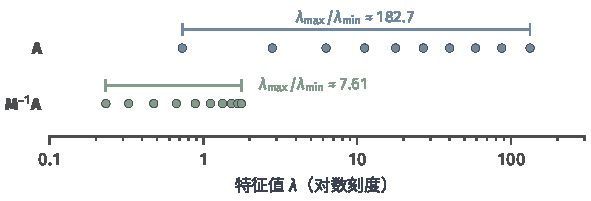
\includegraphics[width=100mm]{figures/01-basic-mathematics/03-vectors-matrices-and-multivariate-functions/matplotlib/c5-preconditioned-spectrum/figure.pdf}
  \caption{对角缩放前后的特征值分布（对数横轴）。矩阵为$\bm A=\bm S\bm T\bm S$，$\bm S=\operatorname{diag}(1,\ldots,10)$，$\bm T$为对角元$1$、次对角元$0.4$的三对角矩阵，预条件$\bm M=\operatorname{diag}(\bm A)$。蓝点为$\bm A$的$10$个特征值（数值计算），绿点为$\bm M^{-1}\bm A$的特征值$1+0.8\cos(j\pi/11)$；括线标出各自的范围与最大、最小特征值之比。}
  \label{fig:ls-preconditioned-spectrum}
\end{figure}

\subsubsection{SSOR预条件}

\paragraph{构造}
对角预条件丢掉了$\bm A$的全部非对角元。要保留更多信息，可以借用第~\ref{sec:ls-ssor}节的SSOR迭代。把对称矩阵写成
\[
 \bm A=\bm D+\bm L+\bm L^\top ,
\]
其中$\bm D$是对角部分，$\bm L$是严格下三角部分。SSOR迭代每一轮先作一次前向扫掠、再作一次反向扫掠，把残差$\bm r_k$变成修正量$\bm\delta_k$（式~\eqref{eq:ls-ssor-correction}）。这一修正是$\bm r_k$的线性函数，记作$\bm\delta_k=\bm M^{-1}\bm r_k$，其中
\begin{equation}
 \bm M=\frac{1}{\omega(2-\omega)}(\bm D+\omega\bm L)\bm D^{-1}(\bm D+\omega\bm L)^\top,\qquad 0<\omega<2 .
 \label{eq:ls-ssor-preconditioner-matrix}
\end{equation}
这个$\bm M$就是SSOR预条件。取$\omega=1$时展开可得
\begin{equation}
 \bm M=(\bm D+\bm L)\bm D^{-1}(\bm D+\bm L^\top)=\bm A+\bm L\bm D^{-1}\bm L^\top ,
 \label{eq:ls-ssor-preconditioner-difference}
\end{equation}
即$\bm M$与$\bm A$只差一项$\bm L\bm D^{-1}\bm L^\top$。

求解$\bm M\bm z=\bm r$不需要形成$\bm M$。记$\bm F=\bm D+\omega\bm L$，它是下三角矩阵，于是$\bm M\bm z=\bm r$可以拆成三步：先解下三角方程，再作对角缩放，最后解上三角方程，
\begin{equation}
 \bm F\bm y=\bm r,\qquad \bm t=\omega(2-\omega)\bm D\bm y,\qquad \bm F^\top\bm z=\bm t .
 \label{eq:ls-ssor-preconditioner}
\end{equation}
三步依次给出$\bm y=\bm F^{-1}\bm r$与$\bm z=\bm F^{-\top}\bm t$，合起来正是
\[
 \bm z=\omega(2-\omega)\bm F^{-\top}\bm D\bm F^{-1}\bm r=\bm M^{-1}\bm r .
\]

例中取$\omega=1$，严格下三角部分与修正项为
\[
 \bm L=\begin{bmatrix}0&0\\1&0\end{bmatrix},\qquad
 \bm L\bm D^{-1}\bm L^\top=\begin{bmatrix}0&0\\0&1/4\end{bmatrix},
\]
所以
\[
 \bm M=\begin{bmatrix}4&1\\1&13/4\end{bmatrix},
\]
它与$\bm A$只在右下角差$1/4$，比对角预条件接近得多。

对$\bm r=(1,2)^\top$求解一次。前代、缩放与回代依次得到
\[
 \bm y=\begin{bmatrix}1/4\\7/12\end{bmatrix},\qquad
 \bm t=\bm D\bm y=\begin{bmatrix}1\\7/4\end{bmatrix},\qquad
 \bm z=\begin{bmatrix}5/48\\7/12\end{bmatrix}.
\]
这正是第~\ref{sec:ls-ssor}节从零初值作一轮SSOR迭代得到的$\bm x_1$。

\paragraph{性质}
SSOR预条件保留了$\bm A$的全部元素，只多出一项$\bm L\bm D^{-1}\bm L^\top$（$\omega=1$时），通常比对角预条件更接近$\bm A$。$\bm A$对称正定且$0<\omega<2$时，$\bm M$也对称正定。它不需要额外存储：所用的三角矩阵$\bm F$就是$\bm A$的下三角部分。每次求解相当于两次三角扫掠，代价约为两次矩阵乘向量；扫掠必须按分量顺序进行，难以并行。$\omega$一经选定，在整个求解过程中就不再改变。

\paragraph{应用场景}
SSOR预条件适合中等规模的对称正定稀疏矩阵，例如椭圆型偏微分方程的离散化：它几乎不需要构造代价，效果又比对角预条件好。预条件的效果对$\omega$不如SSOR迭代本身那样敏感，通常取$\omega=1$，即对称Gauss--Seidel预条件，就已够用。

\subsubsection{不完全分解}

\paragraph{为什么要不完全}
最接近$\bm A$的选择是$\bm A$自己的分解：若$\bm A=\bm L\bm U$，取$\bm M=\bm L\bm U$就有$\bm M=\bm A$，一步即可结束。问题在于，即使$\bm A$很稀疏，它的三角因子也往往稠密得多。消元时，第$i$行减去第$k$行的倍数，会在第$i$行原来为零、而第$k$行不为零的位置上产生新的非零元，称为\term{填充}（fill-in）。填充使存储和三角求解的代价都大大增加。

作为预条件，并不需要精确的因子，只需要$\bm M$接近$\bm A$、三角求解便宜。\term{不完全分解}（incomplete factorization）的做法是：照常执行第~\ref{chap:direct-linear-solvers}章的消元，但事先规定因子允许出现非零元的位置集合$\mathcal S$，消元中凡是落在$\mathcal S$之外的填充一律舍去。最常用的$\mathcal S$就是$\bm A$自身非零元的位置（总含全部对角位置），这时因子与$\bm A$一样稀疏。

\paragraph{不完全LU分解}
回忆第~\ref{sec:ls-lu}节不选主元的LU消元：对$k=1,\ldots,d-1$，用第$k$行消去其下各行的第$k$列元素，
\[
 l_{i,k}=\frac{w_{i,k}}{w_{k,k}},\qquad
 w_{i,j}\leftarrow w_{i,j}-l_{i,k}w_{k,j}\quad(i,j>k),
\]
其中$\bm W$从$\bm A$开始，消元结束时成为$\bm U$。

不完全LU只改动一处：乘子$l_{i,k}$只在$(i,k)\in\mathcal S$时计算，尾块更新只在$(i,j)\in\mathcal S$时执行，其余位置保持为零，相当于把那里产生的填充直接丢掉。为了不破坏规定的稀疏模式，通常不选主元。

结束时得到单位下三角矩阵$\widetilde{\bm L}$与上三角矩阵$\widetilde{\bm U}$，它们的非零元都在$\mathcal S$中，预条件取为
\begin{equation}
 \bm M=\widetilde{\bm L}\widetilde{\bm U} .
 \label{eq:ls-ilu-preconditioner}
\end{equation}
求解$\bm M\bm z=\bm r$就是先解$\widetilde{\bm L}\bm y=\bm r$，再解$\widetilde{\bm U}\bm z=\bm y$，即第~\ref{sec:ls-lu}节的前代~\eqref{eq:ls-forward-substitution}与回代~\eqref{eq:ls-back-substitution}，只是两个因子都是稀疏的。$\bm M$与$\bm A$的差别恰好来自被舍去的填充：若在完整消元中保留它们，所得因子之积就是$\bm A$。

\paragraph{不完全Cholesky分解}
$\bm A$对称正定时，用第~\ref{sec:ls-cholesky}节的Cholesky分解代替LU，得到\term{不完全Cholesky分解}（incomplete Cholesky factorization）。做法相同：按列公式~\eqref{eq:ls-cholesky-columns}逐列计算，但只计算位于$\mathcal S$中的元素，$\mathcal S$之外的元素直接取零。对$j=1,\ldots,d$，
\begin{equation}
 \begin{gathered}
 l_{j,j}=\sqrt{a_{j,j}-\sum_{k<j}l_{j,k}^2},\\
 l_{i,j}=\begin{cases}\dfrac{a_{i,j}-\sum_{k<j}l_{i,k}l_{j,k}}{l_{j,j}},&(i,j)\in\mathcal S,\\[1ex] 0,&(i,j)\notin\mathcal S,\end{cases}\qquad(i>j).
 \end{gathered}
 \label{eq:ls-incomplete-cholesky}
\end{equation}
结束时得到稀疏的下三角矩阵$\bm L$，预条件取为
\begin{equation}
 \bm M=\bm L\bm L^\top ,
 \label{eq:ls-ic-preconditioner}
\end{equation}
求解$\bm M\bm z=\bm r$同样是一次前代与一次回代。不完全Cholesky就是对称情形下的不完全LU：两者舍去的是同样位置上的填充，$\bm L$与$\widetilde{\bm L}$只差各列的一个正的缩放因子。

\paragraph{例子}
二阶的例子没有填充可舍，下面换用
\[
 \bm A=\begin{bmatrix}4&1&1\\1&4&0\\1&0&4\end{bmatrix},
\]
它的$(2,3)$与$(3,2)$元为零，取$\mathcal S$为$\bm A$的非零位置。

先看完整的LU消元。第一步乘子为$l_{2,1}=l_{3,1}=1/4$，第二、三行减去第一行的$1/4$后，
\[
 \bm W=\begin{bmatrix}4&1&1\\0&15/4&-1/4\\0&-1/4&15/4\end{bmatrix}.
\]
原来为零的$(2,3)$与$(3,2)$位置出现了$-1/4$，这就是填充；第二步还要用它算出$l_{3,2}=-1/15$。

不完全LU把这两个填充舍去，第一步后得到
\[
 \bm W=\begin{bmatrix}4&1&1\\0&15/4&0\\0&0&15/4\end{bmatrix},
\]
第二步的乘子$l_{3,2}$不在$\mathcal S$中，取零。于是
\[
 \begin{gathered}
 \widetilde{\bm L}=\begin{bmatrix}1&0&0\\1/4&1&0\\1/4&0&1\end{bmatrix},\\
 \widetilde{\bm U}=\begin{bmatrix}4&1&1\\0&15/4&0\\0&0&15/4\end{bmatrix},
 \end{gathered}
\]
预条件为
\[
 \bm M=\widetilde{\bm L}\widetilde{\bm U}=\begin{bmatrix}4&1&1\\1&4&1/4\\1&1/4&4\end{bmatrix}.
\]
$\bm M$与$\bm A$只在$(2,3)$、$(3,2)$两处不同，差值$1/4$正是被舍去的填充$-1/4$的相反数；两个因子与$\bm A$一样稀疏。

按式~\eqref{eq:ls-incomplete-cholesky}作不完全Cholesky，得
\[
 \bm L=\begin{bmatrix}2&0&0\\1/2&\sqrt{15}/2&0\\1/2&0&\sqrt{15}/2\end{bmatrix},
\]
它的各列是$\widetilde{\bm L}$的各列分别乘以$2,\sqrt{15}/2,\sqrt{15}/2$，所以$\bm L\bm L^\top$给出同一个$\bm M$。

\paragraph{性质}
不完全分解的$\bm M$与$\bm A$的差就是被舍去的填充所产生的影响。$\mathcal S$取得越大，舍去的越少，$\bm M$越接近$\bm A$，效果越好，但因子越稠密，构造与求解的代价也越高；$\mathcal S$取$\bm A$的非零位置是最常见的折中。

不完全分解可能失败。完整Cholesky分解在$\bm A$对称正定时，每一列开方前的量都为正；舍去填充之后，这一保证就不再成立，开方前的量可能为零或为负。所以构造时必须逐列检查，出现非正值时报告失败，或给对角元加上一个正的移位后重新构造。不完全LU也可能遇到零主元。

构造成功时，不完全Cholesky给出的$\bm M$对称正定；不完全LU给出的$\bm M$一般不对称。

\paragraph{应用场景}
不完全分解是一般稀疏矩阵最常用的预条件之一。对称正定矩阵用不完全Cholesky，非对称矩阵用不完全LU。它需要先付出构造代价并存储因子，所以适合条件很差、对角与SSOR预条件不足以显著减少步数的问题，或者需要用同一个矩阵求解多个右端的情形。

\subsection{预条件的使用}
\label{sec:ls-preconditioner-usage}

有了$\bm M$，还要决定$\bm M^{-1}$放在哪里。前面左乘$\bm M^{-1}$只是一种选择，称为左预条件；也可以把$\bm M^{-1}$乘在$\bm A$的右边，称为右预条件：
\begin{equation}
 \bm M^{-1}\bm A\bm x=\bm M^{-1}\bm b,\qquad
 \bm A\bm M^{-1}\bm y=\bm b,\quad \bm x=\bm M^{-1}\bm y .
 \label{eq:ls-left-right-preconditioning}
\end{equation}
由$\bm A\bm M^{-1}=\bm M(\bm M^{-1}\bm A)\bm M^{-1}$，两个矩阵相似，特征值相同，所以从谱的角度看，两种做法加速的效果一样。它们的区别在于求解器看到的残差和未知量是什么，这决定了停止判断是否可靠、最小二乘的目标是否保持。

此外，CG只适用于对称正定矩阵，而$\bm M^{-1}\bm A$与$\bm A\bm M^{-1}$一般都不对称，所以CG需要第三种用法。下面依次讨论这三种用法，每种各取一个求解器，写出带预条件后的计算过程。

\subsubsection{左预条件}

\paragraph{思想}
左预条件求解式~\eqref{eq:ls-left-right-preconditioning}的第一式。未知量仍是$\bm x$，求解器把$\bm M^{-1}\bm A$当作系数矩阵、把$\bm M^{-1}\bm b$当作右端，算法本身一字不改。唯一的变化是：每当求解器需要系数矩阵乘向量$\bm v$时，先算$\bm A\bm v$，再解一次$\bm M\bm w=\bm A\bm v$。这种方式简单直接，GMRES与BiCGSTAB常用它。

它的缺点是改变了残差。求解器算出的残差是
\begin{equation}
 \tilde{\bm r}=\bm M^{-1}\bm b-\bm M^{-1}\bm A\bm x=\bm M^{-1}\bm r ,
 \label{eq:ls-left-preconditioned-residual}
\end{equation}
而不是原方程的残差$\bm r=\bm b-\bm A\bm x$。GMRES最小化的是$\lVert\bm M^{-1}\bm r\rVert_2$，按递推估计停止时，阈值检查的也是这个量；它与$\lVert\bm r\rVert_2$可以相差很多，最多可差$\bm M$的条件数倍。所以停止前必须用$\bm b-\bm A\bm x$重新计算原残差并复核。

对不相容的最小二乘问题，改变残差就改变了目标：
\[
 \lVert\bm M^{-1}(\bm b-\bm A\bm x)\rVert_2^2=(\bm b-\bm A\bm x)^\top\bm M^{-\top}\bm M^{-1}(\bm b-\bm A\bm x)
\]
是第~\ref{sec:ls-weighted-ls}节以$\bm M^{-\top}\bm M^{-1}$为权的加权最小二乘，一般会得到不同的解。所以最小二乘求解器不用左预条件。

MINRES也属于这一类，但它要求系数矩阵对称，而$\bm M^{-1}\bm A$不对称。它的预条件版本取对称正定的$\bm M$，把通常的内积换成$\bm M$诱导的内积，最小化的是$(\bm r^\top\bm M^{-1}\bm r)^{1/2}$，同样不是原残差的长度。

\paragraph{计算过程：左预条件GMRES}
与第~\ref{sec:ls-gmres}节相比，只有两处改动：初始残差换成预条件残差，Arnoldi扩展中的矩阵乘向量后接一次辅助求解。每一步使用例~\ref{ex:ls-stationary-running-example}的数据进行演示：
\[
 \bm A=\begin{bmatrix}4&1\\1&3\end{bmatrix},\qquad
 \bm b=\begin{bmatrix}1\\2\end{bmatrix},\qquad
 \bm x_0=\bm 0 .
\]
取对角预条件$\bm M=\operatorname{diag}(4,3)$，于是
\[
 \widetilde{\bm A}=\bm M^{-1}\bm A=\begin{bmatrix}1&1/4\\1/3&1\end{bmatrix}.
\]

\paragraph{变量}
\begin{itemize}
 \item 第~\ref{sec:ls-gmres}节的全部变量：周期起点$\bm x^{(s)}$、基$\bm v_1,\ldots,\bm v_{j+1}$、工作向量$\bm w$、$\overline{\bm H}_j$的各列、旋转$c_i,s_i$与右端$\bm g$；其中$\bm v_i$是$\mathcal K_j(\widetilde{\bm A},\tilde{\bm r}_0)$的基，$\lvert g_{j+1}\rvert$估计的是预条件残差的长度。
 \item 预条件$\bm M$：只用于求解$\bm M\bm z=\bm r$。
\end{itemize}

\paragraph{初始化}
把预条件残差初始化为$\tilde{\bm r}_0=\bm M^{-1}(\bm b-\bm A\bm x_0)$，其余与GMRES相同：
\[
 \beta=\lVert\tilde{\bm r}_0\rVert_2,\qquad \bm v_1=\frac{\tilde{\bm r}_0}{\beta},\qquad g_1=\beta,\qquad j=1 .
\]
例中$\tilde{\bm r}_0=(1/4,2/3)^\top$，
\[
 \beta=\frac{\sqrt{73}}{12}\approx0.7120,\qquad \bm v_1=\frac1{\sqrt{73}}\begin{bmatrix}3\\8\end{bmatrix}.
\]

\paragraph{每轮更新}
在第$j$轮：
\begin{enumerate}
 \item \textbf{乘矩阵并作辅助求解。}计算$\bm A\bm v_j$，再解
 \[
  \bm M\bm w=\bm A\bm v_j ,
 \]
 得到$\bm w=\widetilde{\bm A}\bm v_j$。例中第一轮$\bm A\bm v_1=(20,27)^\top/\sqrt{73}$，逐分量相除得
 \[
  \bm w=\frac1{\sqrt{73}}\begin{bmatrix}5\\9\end{bmatrix}.
 \]

 \item \textbf{Arnoldi正交化。}对$\bm w$按第~\ref{sec:ls-arnoldi}节的式~\eqref{eq:ls-arnoldi-coefficients}与\eqref{eq:ls-arnoldi-normalize}正交化并归一化，得到$\overline{\bm H}_j$的第$j$列与$\bm v_{j+1}$。例中第一轮
 \[
  h_{1,1}=\frac{87}{73},\qquad h_{2,1}=\frac{13}{73},\qquad \bm v_2=\frac1{\sqrt{73}}\begin{bmatrix}8\\-3\end{bmatrix}.
 \]

 \item \textbf{旋转与右端。}按第~\ref{sec:ls-gmres}节每轮更新的第2—4步，对新列作用旧旋转、构造新旋转，并按式~\eqref{eq:ls-gmres-rhs}更新右端。例中第一轮
 \[
  \rho_1=\frac{\sqrt{7738}}{73}\approx1.2050,\qquad
  \lvert g_2\rvert=\frac{\beta h_{2,1}}{\rho_1}=\frac{13}{12\sqrt{106}}\approx0.1052 .
 \]
 若此时回代，得
 \[
  \bm x_1=\begin{bmatrix}87/424\\29/53\end{bmatrix}\approx\begin{bmatrix}0.2052\\0.5472\end{bmatrix},
 \]
 它的原残差
 \[
  \bm r_1=\bm b-\bm A\bm x_1=\begin{bmatrix}-39/106\\65/424\end{bmatrix},\qquad \lVert\bm r_1\rVert_2\approx0.3986,
 \]
 而$\lVert\bm M^{-1}\bm r_1\rVert_2\approx0.1052$恰为$\lvert g_2\rvert$：GMRES报告的残差比原残差小了将近$4$倍。

 例中第二轮由第1步，
 \[
  \bm A\bm v_2=\frac1{\sqrt{73}}\begin{bmatrix}29\\-1\end{bmatrix},\qquad
  \bm w=\frac1{\sqrt{73}}\begin{bmatrix}29/4\\-1/3\end{bmatrix};
 \]
 由第2步，
 \[
  h_{1,2}=\frac{229}{876},\qquad h_{2,2}=\frac{59}{73},\qquad h_{3,2}=0 ,
 \]
 于是$g_3=0$。

 \item \textbf{停止。}若$\lvert g_{j+1}\rvert\le\tau$、$h_{j+1,j}=0$或已达到步数上限，退出每轮更新，按GMRES回代并还原$\bm x$；由于$\lvert g_{j+1}\rvert$度量的是预条件残差，退出后必须用$\bm b-\bm A\bm x$复核原残差，按第~\ref{sec:ls-stationary-stopping}节判断是否达到容差。

 例中第二轮$h_{3,2}=0$，退出迭代。
\end{enumerate}

最终回代得
\[
 \bm x_2=\bm x_\star=\begin{bmatrix}1/11\\7/11\end{bmatrix},
\]
复核原残差为零。与无预条件的GMRES相比，两者都两步结束；第一步的原残差由$0.542$降到$0.399$，但停止判断所用的估计$0.105$与原残差并不相等，这就是左预条件对残差的扭曲。

\subsubsection{右预条件}

\paragraph{思想}
右预条件求解式~\eqref{eq:ls-left-right-preconditioning}的第二式。求解器把$\bm A\bm M^{-1}$当作系数矩阵，未知量换成$\bm y=\bm M\bm x$。每当需要系数矩阵乘向量$\bm v$时，先解一次$\bm M\bm z=\bm v$，再算$\bm A\bm z$。

这样做的好处是残差不变。对任意$\bm y$，记$\bm x=\bm M^{-1}\bm y$，有
\begin{equation}
 \bm b-\bm A\bm M^{-1}\bm y=\bm b-\bm A\bm x ,
 \label{eq:ls-right-preconditioned-residual}
\end{equation}
所以求解器算出的残差就是原方程的真实残差。GMRES这类最小残差方法最小化的正是$\lVert\bm b-\bm A\bm x\rVert_2$，递推估计与停止阈值都直接针对它；对最小二乘问题，目标$\lVert\bm b-\bm A\bm x\rVert_2$与解集也都保持不变。

右预条件的另一个特点是变量解耦。整个迭代只在$\bm y$上进行，$\bm M$只出现在系数矩阵的作用里，不进入解的递推；原变量$\bm x$只在结束时由一次求解$\bm M\bm x=\bm y$得到。

因此，LSQR与LSMR采用右预条件；GMRES需要直接控制原残差时也常用它。LSQR与LSMR还要用到系数矩阵的转置乘向量，这时$(\bm A\bm M^{-1})^\top\bm u=\bm M^{-\top}(\bm A^\top\bm u)$，即先乘$\bm A^\top$，再解一次$\bm M^\top\bm z=\bm A^\top\bm u$。

有两点需要注意。

其一，LSQR报告的正规残差估计变成了$\lVert\bm M^{-\top}\bm A^\top\bm r\rVert_2$，不再是$\lVert\bm A^\top\bm r\rVert_2$。

其二，零初值下LSQR选出的是$\lVert\bm y\rVert_2=\lVert\bm M\bm x\rVert_2$最小的最小二乘解；$\bm A$秩亏时，它未必是原坐标下欧氏范数最小的那个解。

\paragraph{计算过程：右预条件LSQR}
与第~\ref{sec:ls-lsqr}节相比，双对角化中的两次矩阵作用各接一次辅助求解，解的累加改在$\bm y$上进行，结束时换回$\bm x$。每一步使用第~\ref{sec:ls-lsqr}节的不相容系统进行演示：
\[
 \bm A=\begin{bmatrix}1&0\\0&2\\0&0\end{bmatrix},\qquad
 \bm b=\begin{bmatrix}1\\1\\1\end{bmatrix},
\]
取列缩放$\bm M=\operatorname{diag}(\lVert\bm a_1\rVert_2,\lVert\bm a_2\rVert_2)=\operatorname{diag}(1,2)$，于是
\[
 \widehat{\bm A}=\bm A\bm M^{-1}=\begin{bmatrix}1&0\\0&1\\0&0\end{bmatrix}
\]
的两列已是标准正交的。

\paragraph{变量}
\begin{itemize}
 \item 第~\ref{sec:ls-lsqr}节的全部变量：基向量$\bm u,\bm v$，双对角系数$\alpha,\beta$，正交变换的$\rho,\bar\rho,c,s,\theta,\phi,\bar\phi$与方向$\bm w$；它们都针对$\widehat{\bm A}$。
 \item $\bm y\in\mathbb R^d$：$\bm y$坐标下的近似解，代替LSQR中的$\bm x$累加。
 \item 预条件$\bm M$：用于求解$\bm M\bm z=\bm v$与$\bm M^\top\bm z=\bm A^\top\bm u$。
\end{itemize}

\paragraph{初始化}
按式~\eqref{eq:ls-golub-kahan-start}起步，其中$\widehat{\bm A}^\top\bm u_1=\bm M^{-\top}(\bm A^\top\bm u_1)$；把$\bm y$初始化为零，其余与LSQR相同：
\[
 \bm y_0=\bm 0,\qquad \bm w_1=\bm v_1,\qquad \bar\rho_1=\alpha_1,\qquad \bar\phi_1=\beta_1 .
\]
例中$\beta_1=\sqrt3$，$\bm u_1=(1,1,1)^\top/\sqrt3$。先乘$\bm A^\top$，再作辅助求解，得
\[
 \bm A^\top\bm u_1=\frac1{\sqrt3}\begin{bmatrix}1\\2\end{bmatrix},\qquad
 \widehat{\bm A}^\top\bm u_1=\bm M^{-\top}(\bm A^\top\bm u_1)=\frac1{\sqrt3}\begin{bmatrix}1\\1\end{bmatrix},
\]
故
\[
 \alpha_1=\sqrt{\frac23},\qquad \bm v_1=\frac1{\sqrt2}\begin{bmatrix}1\\1\end{bmatrix}.
\]

\paragraph{每轮更新}
在第$k$轮：
\begin{enumerate}
 \item \textbf{带辅助求解的双对角化。}按式~\eqref{eq:ls-golub-kahan-step}扩展一步，其中
 \begin{equation}
  \widehat{\bm A}\bm v_k=\bm A(\bm M^{-1}\bm v_k),\qquad \widehat{\bm A}^\top\bm u_{k+1}=\bm M^{-\top}(\bm A^\top\bm u_{k+1}).
  \label{eq:ls-preconditioned-lsqr-products}
 \end{equation}
 例中第一轮先作辅助求解，再乘$\bm A$，
 \[
  \bm M^{-1}\bm v_1=\frac1{\sqrt2}\begin{bmatrix}1\\1/2\end{bmatrix},\qquad
  \widehat{\bm A}\bm v_1=\frac1{\sqrt2}\begin{bmatrix}1\\1\\0\end{bmatrix},
 \]
 扣除$\alpha_1\bm u_1$后
 \[
  \beta_2=\frac1{\sqrt3},\qquad \bm u_2=\frac1{\sqrt6}\begin{bmatrix}1\\1\\-2\end{bmatrix};
 \]
 $\widehat{\bm A}^\top\bm u_2=(1,1)^\top/\sqrt6$恰好等于$\beta_2\bm v_1$，所以$\alpha_2=0$。

 \item \textbf{正交变换。}按式~\eqref{eq:ls-lsqr-rotation}消去$\beta_{k+1}$。例中第一轮
 \[
  \begin{gathered}
  \rho_1=1,\qquad c_1=\sqrt{\frac23},\qquad s_1=\frac1{\sqrt3},\\
  \theta_2=0,\qquad \phi_1=\sqrt2,\qquad \bar\phi_2=1 .
  \end{gathered}
 \]

 \item \textbf{在$\bm y$坐标中更新解与方向。}按式~\eqref{eq:ls-lsqr-update}与\eqref{eq:ls-lsqr-direction}，把其中的$\bm x$换成$\bm y$：
 \[
  \bm y_k=\bm y_{k-1}+\frac{\phi_k}{\rho_k}\bm w_k,\qquad \bm w_{k+1}=\bm v_{k+1}-\frac{\theta_{k+1}}{\rho_k}\bm w_k .
 \]
 例中第一轮
 \[
  \bm y_1=\sqrt2\,\bm w_1=\begin{bmatrix}1\\1\end{bmatrix}.
 \]

 \item \textbf{停止。}按式~\eqref{eq:ls-lsqr-estimates}读出两个估计：$\lvert\bar\phi_{k+1}\rvert$就是原残差的长度，另一个是$\lVert\bm M^{-\top}\bm A^\top\bm r_k\rVert_2$。达到阈值、出现零系数或步数用尽时退出，换回$\bm x_k=\bm M^{-1}\bm y_k$并复核真实残差。

 例中第一轮原残差估计为$1$，正规残差估计为$\lvert\bar\phi_2\rvert\alpha_2\lvert c_1\rvert=0$，且$\alpha_2=0$，退出迭代。
\end{enumerate}

最终换回原变量
\[
 \bm x_1=\bm M^{-1}\bm y_1=\begin{bmatrix}1\\1/2\end{bmatrix}=\hat{\bm x},
\]
真实残差为$(0,0,1)^\top$，长度恰为估计值$1$：右预条件下递推看到的就是原残差。

无预条件的LSQR在这个例子上需要两轮（第~\ref{sec:ls-lsqr}节）；列缩放使$\widehat{\bm A}$的列标准正交，一轮即得最小二乘解。

\subsubsection{预条件共轭梯度法}
\label{sec:ls-pcg}

\paragraph{CG对$\bm M$的要求}
CG要求系数矩阵对称正定，左、右预条件都不满足这一点：即使$\bm A$与$\bm M$都对称正定，$\bm M^{-1}\bm A$与$\bm A\bm M^{-1}$一般也不对称。左预条件GMRES的例子中
\[
 \bm M^{-1}\bm A=\begin{bmatrix}1&1/4\\1/3&1\end{bmatrix}
\]
就不对称。对这样的矩阵，CG的残差正交与方向共轭都不再成立。

所以用于CG的预条件需要另作处理。

首先，$\bm M$本身必须对称正定，并在整个迭代中固定不变；对角预条件、SSOR预条件以及构造成功的不完全Cholesky都满足这一点，不完全LU则一般不满足。

其次，$\bm M^{-1}$不能只乘在一侧，而要把$\bm M$拆成两个互为转置的因子，分别乘在$\bm A$的两侧，使变换后的矩阵仍然对称正定。

\paragraph{保持对称的变换}
设$\bm A$与$\bm M$都对称正定，写$\bm M=\bm C\bm C^\top$，代换$\bm x=\bm C^{-\top}\bm y$并左乘$\bm C^{-1}$，得到
\begin{equation}
 \widehat{\bm A}\bm y=\bm C^{-1}\bm b,\qquad \widehat{\bm A}=\bm C^{-1}\bm A\bm C^{-\top},
 \label{eq:ls-pcg-transformed-system}
\end{equation}
其中$\widehat{\bm A}$对称正定：对$\bm w\neq\bm0$有
\[
 \bm w^\top\widehat{\bm A}\bm w=(\bm C^{-\top}\bm w)^\top\bm A(\bm C^{-\top}\bm w)>0 ,
\]
可以施行CG。$\widehat{\bm A}=\bm C^\top(\bm M^{-1}\bm A)\bm C^{-\top}$与$\bm M^{-1}\bm A$相似，所以改善的正是$\bm M^{-1}\bm A$的谱。

\paragraph{递推}
对式~\eqref{eq:ls-pcg-transformed-system}施行CG再换回原变量（定理~\ref{thm:ls-pcg-equivalence}），$\bm C$从公式中消失，得到\term{预条件共轭梯度法}（preconditioned conjugate gradient method，PCG）。记预条件残差$\bm z_k=\bm M^{-1}\bm r_k$与配对量$\tau_k=\bm r_k^\top\bm z_k$，步长与组合系数为
\begin{equation}
 \alpha_k=\frac{\tau_k}{\bm p_k^\top\bm A\bm p_k},\qquad \beta_k=\frac{\tau_{k+1}}{\tau_k},
 \label{eq:ls-pcg-coefficients}
\end{equation}
解、残差与方向按
\begin{equation}
 \begin{gathered}
 \bm x_{k+1}=\bm x_k+\alpha_k\bm p_k,\qquad
 \bm r_{k+1}=\bm r_k-\alpha_k\bm A\bm p_k,\\
 \bm p_0=\bm z_0,\qquad \bm p_{k+1}=\bm z_{k+1}+\beta_k\bm p_k
 \end{gathered}
 \label{eq:ls-pcg-updates}
\end{equation}
更新。与CG的式~\eqref{eq:ls-cg-update}—\eqref{eq:ls-cg-beta}相比，只是新方向由$\bm z$而不是$\bm r$组合而成，内积$\bm r^\top\bm r$换成$\bm r^\top\bm z$；递推中的残差仍是原残差，停止判断不受扭曲。每轮比CG多一次辅助求解$\bm M\bm z_{k+1}=\bm r_{k+1}$。

\begin{theorem}[PCG与变换后CG的等价]
\label{thm:ls-pcg-equivalence}
设$\bm A,\bm M$对称正定，$\bm M=\bm C\bm C^\top$，$\widehat{\bm A}=\bm C^{-1}\bm A\bm C^{-\top}$。在精确算术中，只要PCG尚未终止，它的迭代量与对$\widehat{\bm A}\bm y=\bm C^{-1}\bm b$从$\bm y_0=\bm C^\top\bm x_0$施行CG所得的迭代量满足
\begin{equation}
 \bm y_k=\bm C^\top\bm x_k,\qquad \hat{\bm r}_k=\bm C^{-1}\bm r_k,\qquad \hat{\bm p}_k=\bm C^\top\bm p_k .
 \label{eq:ls-pcg-correspondence}
\end{equation}
因此$\bm x_k$是$\bm x_0+\mathcal K_k(\bm M^{-1}\bm A,\bm M^{-1}\bm r_0)$中使$\lVert\bm x-\bm x_\star\rVert_{\bm A}$最小的唯一点，并且
\begin{equation}
 \begin{gathered}
 \lVert\bm x_k-\bm x_\star\rVert_{\bm A}\le2\Bigl(\frac{\sqrt{\hat\kappa}-1}{\sqrt{\hat\kappa}+1}\Bigr)^k\lVert\bm x_0-\bm x_\star\rVert_{\bm A},\\
 \hat\kappa=\kappa_2(\widehat{\bm A})=\frac{\lambda_{\max}(\bm M^{-1}\bm A)}{\lambda_{\min}(\bm M^{-1}\bm A)} .
 \end{gathered}
 \label{eq:ls-pcg-convergence-bound}
\end{equation}
\end{theorem}

\begin{proof}
先对$k$归纳证明迭代量的对应关系，再把CG的最优性与收敛界换回原变量。

\emph{起点。}由$\widehat{\bm A}$的定义，
\[
 \hat{\bm r}_0=\bm C^{-1}\bm b-\widehat{\bm A}\bm C^\top\bm x_0=\bm C^{-1}\bm r_0 ,
\]
而$\bm C^{-\top}\bm C^{-1}=\bm M^{-1}$，故
\[
 \hat{\bm p}_0=\hat{\bm r}_0=\bm C^\top(\bm M^{-1}\bm r_0)=\bm C^\top\bm z_0=\bm C^\top\bm p_0 .
\]

\emph{系数相同。}设第$k$步对应关系成立。CG步长中的两个内积逐项换算为
\[
 \begin{aligned}
 \hat{\bm r}_k^\top\hat{\bm r}_k&=\bm r_k^\top\bm M^{-1}\bm r_k=\tau_k,\\
 \hat{\bm p}_k^\top\widehat{\bm A}\hat{\bm p}_k&=\bm p_k^\top\bm C\bigl(\bm C^{-1}\bm A\bm C^{-\top}\bigr)\bm C^\top\bm p_k=\bm p_k^\top\bm A\bm p_k ,
 \end{aligned}
\]
所以CG的步长等于式~\eqref{eq:ls-pcg-coefficients}的$\alpha_k$；同理组合系数同为$\tau_{k+1}/\tau_k$。

\emph{迭代量对应。}系数相同，于是
\[
 \bm y_{k+1}=\bm C^\top(\bm x_k+\alpha_k\bm p_k)=\bm C^\top\bm x_{k+1} .
\]
再由$\widehat{\bm A}\hat{\bm p}_k=\bm C^{-1}\bm A\bm p_k$得
\[
 \begin{aligned}
 \hat{\bm r}_{k+1}&=\bm C^{-1}(\bm r_k-\alpha_k\bm A\bm p_k)=\bm C^{-1}\bm r_{k+1},\\
 \hat{\bm p}_{k+1}&=\bm C^{-1}\bm r_{k+1}+\beta_k\bm C^\top\bm p_k\\
 &=\bm C^\top(\bm z_{k+1}+\beta_k\bm p_k)=\bm C^\top\bm p_{k+1}.
 \end{aligned}
\]

\emph{最优性与收敛界。}由定理~\ref{thm:ls-cg-convergence}，$\bm y_k$是$\bm y_0+\mathcal K_k(\widehat{\bm A},\hat{\bm r}_0)$中使$\lVert\bm y-\bm C^\top\bm x_\star\rVert_{\widehat{\bm A}}$最小的唯一点。换回$\bm x=\bm C^{-\top}\bm y$时，
\[
 \begin{gathered}
 \lVert\bm C^\top(\bm x-\bm x_\star)\rVert_{\widehat{\bm A}}=\lVert\bm x-\bm x_\star\rVert_{\bm A},\\
 \bm C^{-\top}\widehat{\bm A}^j\hat{\bm r}_0=(\bm M^{-1}\bm A)^j\bm M^{-1}\bm r_0 ,
 \end{gathered}
\]
所以仿射子空间和目标都对应过来，收敛界也随之成立。最后，$\bm M^{-1}\bm A=\bm C^{-\top}\widehat{\bm A}\bm C^\top$与$\widehat{\bm A}$相似，而$\widehat{\bm A}$对称正定，$\kappa_2(\widehat{\bm A})$就是特征值之比。
\end{proof}

定理中的$\bm C$只用于论证，算法只需求解$\bm M\bm z=\bm r$；收敛速度由$\bm M^{-1}\bm A$的特征值之比$\hat\kappa$决定，图~\ref{fig:ls-preconditioned-spectrum}中对角缩放把它从约$182.7$降到约$7.61$。论证要求整个迭代使用同一个固定的线性作用$\bm M^{-1}$；预条件随轮次变化时，标准PCG的共轭性与最优性不再沿用。

\paragraph{计算过程}
下面写出PCG的计算过程。每一步使用例~\ref{ex:ls-stationary-running-example}的数据进行演示：
\[
 \bm A=\begin{bmatrix}4&1\\1&3\end{bmatrix},\qquad
 \bm b=\begin{bmatrix}1\\2\end{bmatrix},\qquad
 \bm x_0=\bm0 .
\]
精确解为$\bm x_\star=(1/11,7/11)^\top$。预条件取对角预条件$\bm M=\operatorname{diag}(4,3)$，它对称正定，满足上面的要求。

预先选定的参数为$\mathrm{atol},\mathrm{rtol},K$；停止检查沿用第~\ref{sec:ls-stationary-stopping}节，按原残差判断。这里的$\alpha_k,\beta_k$是CG的步长与组合系数，与双对角化的系数无关。

\paragraph{变量}
\begin{itemize}
 \item $\bm x\in\mathbb R^d$：当前近似解。
 \item $\bm r\in\mathbb R^d$：原残差$\bm b-\bm A\bm x$。
 \item $\bm z\in\mathbb R^d$：预条件残差，即辅助方程$\bm M\bm z=\bm r$的解。
 \item $\bm p\in\mathbb R^d$：搜索方向。
 \item $\bm q\in\mathbb R^d$：工作向量，存放$\bm A\bm p$。
 \item $\tau_k=\bm r_k^\top\bm z_k$：配对量，留到下一轮求$\beta_k$时使用；$\alpha_k,\beta_k$：步长与组合系数。
 \item $k$：轮次。
\end{itemize}
除矩阵与预条件外只保存$\bm x,\bm r,\bm z,\bm p,\bm q$五个向量。

\paragraph{初始化}
把残差初始化为$\bm r_0=\bm b-\bm A\bm x_0$；若已达到原残差容差或$K=0$，直接输出$\bm x_0$。否则求解$\bm M\bm z_0=\bm r_0$，把方向初始化为预条件残差，轮次初始化为$0$：
\[
 \bm p_0=\bm z_0,\qquad \tau_0=\bm r_0^\top\bm z_0,\qquad k=0 .
\]
例中$\bm r_0=(1,2)^\top$，按式~\eqref{eq:ls-diagonal-preconditioner}逐分量相除，
\[
 \bm z_0=\bm p_0=\begin{bmatrix}1/4\\2/3\end{bmatrix},\qquad
 \tau_0=1\cdot\frac14+2\cdot\frac23=\frac{19}{12}.
\]

\paragraph{每轮更新}
在第$k$轮：
\begin{enumerate}
 \item \textbf{乘矩阵并求步长。}作本轮唯一的矩阵乘向量，按式~\eqref{eq:ls-pcg-coefficients}求步长：
 \[
  \bm q_k=\bm A\bm p_k,\qquad \alpha_k=\frac{\tau_k}{\bm p_k^\top\bm q_k}.
 \]
 例中第一轮
 \[
  \bm q_0=\begin{bmatrix}5/3\\9/4\end{bmatrix},\qquad \bm p_0^\top\bm q_0=\frac5{12}+\frac32=\frac{23}{12},\qquad \alpha_0=\frac{19}{23}.
 \]

 \item \textbf{更新解与残差。}按式~\eqref{eq:ls-pcg-updates}，其中$\bm A\bm p_k$直接取$\bm q_k$：
 \[
  \bm x_{k+1}=\bm x_k+\alpha_k\bm p_k,\qquad \bm r_{k+1}=\bm r_k-\alpha_k\bm q_k .
 \]
 例中第一轮
 \[
  \begin{gathered}
  \bm x_1=\begin{bmatrix}19/92\\38/69\end{bmatrix}\approx\begin{bmatrix}0.2065\\0.5507\end{bmatrix},\\
  \bm r_1=\begin{bmatrix}1\\2\end{bmatrix}-\frac{19}{23}\begin{bmatrix}5/3\\9/4\end{bmatrix}=\begin{bmatrix}-26/69\\13/92\end{bmatrix},
  \end{gathered}
 \]
 直接计算$\bm b-\bm A\bm x_1$得到同一残差，$\lVert\bm r_1\rVert_2\approx0.402$。

 CG最小化的误差$\lVert\bm x-\bm x_\star\rVert_{\bm A}$从初值处的$\sqrt{15/11}\approx1.168$降到约$0.236$；同一初值下普通CG的第一步是$(1/4,1/2)^\top$，这一误差约为$0.337$。

 \item \textbf{预条件求解。}求解辅助方程并更新配对量：
 \[
  \bm M\bm z_{k+1}=\bm r_{k+1},\qquad \tau_{k+1}=\bm r_{k+1}^\top\bm z_{k+1}.
 \]
 例中第一轮
 \[
  \bm z_1=\begin{bmatrix}-13/138\\13/276\end{bmatrix},\qquad
  \tau_1=\frac{3211}{76176}.
 \]

 \item \textbf{形成新方向。}按式~\eqref{eq:ls-pcg-coefficients}与\eqref{eq:ls-pcg-updates}，
 \[
  \beta_k=\frac{\tau_{k+1}}{\tau_k},\qquad \bm p_{k+1}=\bm z_{k+1}+\beta_k\bm p_k ,
 \]
 然后令$k\leftarrow k+1$。$\bm A$与$\bm M$正定保证正常步骤中$\tau_k$与$\bm p_k^\top\bm q_k$两个分母为正。

 例中第一轮
 \[
  \beta_0=\frac{\tau_1}{\tau_0}=\frac{169}{6348},\qquad
  \bm p_1=\bm z_1+\beta_0\bm p_0=\begin{bmatrix}-741/8464\\1235/19044\end{bmatrix}.
 \]

 例中第二轮的步长为
 \[
  \alpha_1=\frac{\tau_1}{\bm p_1^\top\bm q_1}=\frac{276}{209},
 \]
 由此得到
 \[
  \bm x_2=\bm x_1+\frac{276}{209}\bm p_1=\begin{bmatrix}1/11\\7/11\end{bmatrix},\qquad \bm r_2=\bm 0 .
 \]

 \item \textbf{停止。}在第2步之后按第~\ref{sec:ls-stationary-stopping}节检查原残差$\bm r_{k+1}$，满足阈值或$k+1=K$时退出并输出$\bm x_{k+1}$，退出前用$\bm b-\bm A\bm x_{k+1}$复核递推残差；检查放在预条件求解之前，残差为零时先结束，不再计算$\tau_{k+1}$。若未收敛时出现非正的$\tau_k$或$\bm p_k^\top\bm q_k$，应检查$\bm A,\bm M$的正定前提与数值状态，报告异常并退出。

 例中第二轮$\bm r_2=\bm 0$，退出迭代。
\end{enumerate}

最终得到
\[
 \bm x_2=\bm x_\star=\begin{bmatrix}1/11\\7/11\end{bmatrix},
\]
与二维问题至多两步结束一致；两轮共做了两次辅助求解与两次矩阵乘向量，复核残差另计。

普通CG在这个问题上也是两步结束，所以本例只用来核对公式；预条件的收益要看$\bm M^{-1}\bm A$的谱，并与构造和应用$\bm M$的代价一起比较达到同一精度的总工作量。预条件只改善迭代面对的谱，不改变原问题对数据的敏感度。

\FloatBarrier
\section{本章小结}
\label{sec:krylov-methods-summary}

本章从定常迭代每轮丢弃历史信息这一缺点出发，把初始残差及其矩阵乘积张成的Krylov子空间保留下来，在逐步扩大的仿射空间$\bm x_0+\mathcal K_k$中选取近似。选一个近似等价于选一个在原点取值$1$的残差多项式；各方法的区别在于按什么准则选这个多项式，以及怎样用性质良好的基而不是病态的幂向量完成计算。由于系数随当前向量变化，收敛性都由各自的选解准则推出，而不是由固定误差矩阵的谱半径判断。

方阵上的方法按矩阵类型分工。对称矩阵（可以不定）用MINRES，借Lanczos过程的三项递推与带状QR，在固定存储下最小化原残差，收敛界只依赖特征值。对称正定矩阵还可用CG，它在当前子空间中最小化误差的能量范数，步长与组合系数都可由残差长度算出，短递推在精确算术下保持全部正交与共轭关系，误差界由$\sqrt{\kappa_2(\bm A)}$控制。一般方阵用GMRES，它在Arnoldi关系给出的小问题上最小化原残差，残差单调不增，但基的存储与正交化工作随步数增长；重启限制了存储，也失去了跨周期的最优性，可能停滞。

非对称矩阵若要固定存储，就要放弃残差最小化。BiCG用原矩阵与转置矩阵维持双正交和双共轭，系数公式与CG同形，但残差可能波动，配对量为零时递推中断。BiCGSTAB用固定影子向量代替影子序列，方向的组合系数由残差多项式的首项系数比推出，再加一次局部最小残差步；每轮只用$\bm A$，局部改进只相对于中间残差成立，既不保证整轮单调，也不消除中断。

长方或秩亏的最小二乘问题用LSQR与LSMR。LSQR在$\mathcal K_k(\bm A^\top\bm A,\bm A^\top\bm b)$中最小化原残差，精确算术下等价于正规方程上的CG；LSMR最小化正规残差，等价于正规方程上的MINRES，需要两层正交变换和两套方向。两者都取零初值，到达正规方程时选出最小范数解$\bm A^\dagger\bm b$；它们避免了形成Gram矩阵时的信息损失，但收敛快慢仍由非零奇异值平方的分布决定，原问题的病态性也不因算法而消失。

这些求解方法共用三个底层子空间工具，它们放在所有求解方法之前讨论；它们给出的基与小矩阵只是求解器的中间量。Arnoldi正交化对一般方阵把$\bm A\bm v_j$与全部已有基向量正交化，生成Krylov子空间的标准正交基，并把$\bm A$压缩成上Hessenberg矩阵$\bm H_k=\bm V_k^\top\bm A\bm V_k$；原方程在子空间中化为小问题，按极小残差条件求解就是GMRES，代价是整组基都要保存。

Lanczos过程是它在对称矩阵上的简化：被省略的系数本来为零，每轮只扣除最近两个方向，小矩阵成为对称三对角矩阵；MINRES直接在这个小矩阵上选解，CG的残差与Lanczos向量平行，其短递推相当于逐步延续三对角矩阵的$\bm L\bm D\bm L^\top$分解。

Golub--Kahan双对角化交替作用$\bm A$与$\bm A^\top$，在两个空间各得一组标准正交基，把$\bm A$压缩成下双对角矩阵，右侧基张成$\mathcal K_k(\bm A^\top\bm A,\bm A^\top\bm b)$，却从不形成$\bm A^\top\bm A$，供LSQR与LSMR使用。

预条件是一种加速与预处理手段，用一个易解的$\bm M$改变迭代面对的谱：对角缩放、SSOR与不完全分解分别复用前几章的公式，PCG则是对称正定变换系统上的CG，换回原变量后只需每轮多解一次$\bm M\bm z=\bm r$。选用时要同时计入构造与应用的代价，并核对变换是否保持了方法的前提和原来的求解目标：PCG与MINRES需要对称正定的$\bm M$，左预条件会改变残差的度量，右预条件在秩亏时可能改变最小范数的选解。

最后，所有方法都以真实残差决定是否成功：方阵问题检查原残差，不相容最小二乘问题检查正规残差而允许原残差非零。递推得到的残差估计只是复核的提示；达到步数上限、停滞和中断都要与达到精度区分开。残差小到什么程度才说明解可信，取决于问题的条件数，这一问题以及在同一目标下怎样比较本章与前几章的方法，留给第~\ref{chap:solution-error-regularization}章。

